\documentclass[10pt]{article}
\usepackage[margin=2.2cm]{geometry}
\usepackage{booktabs,longtable,graphicx,array}
\usepackage[hidelinks]{hyperref}
\setlength{\tabcolsep}{4pt}
\newcommand{\stackcell}[1]{\begin{tabular}[t]{@{}l@{}}#1\end{tabular}}
\title{tropical: MinCoinChange}
\date{2026-10-25T15:59:14}
\begin{document}
\maketitle

\section{Key results}
This report covers 240 runs (5 seeds; 0 diverged) under frozen hash \texttt{7237e0b98779}.
\paragraph{Where to look.} The headline metric is \texttt{ood\_len\_f1} (higher is better).
\autoref{fig:ood_len_f1} plots it against \texttt{fishr\_lambda}.
\autoref{tab:summary-ood_len_f1} gives every cell's mean with its 95\% bootstrap CI.
\autoref{tab:control-ood_len_f1} compares each level with the control.
\autoref{tab:trend-ood_len_f1} gives the trend.
\autoref{tab:paired-ood_len_f1} gives the paired contrasts.
Its tests take the parametric path: values away from the metric bounds.
Cells are compared within a seed: a seed index fixes the data and the initialization.
Comparisons are marked significant at $p < 0.05$ after the stated correction.

\subsection{\texttt{ood\_len\_f1}}
\begin{figure}[tbp]
\centering
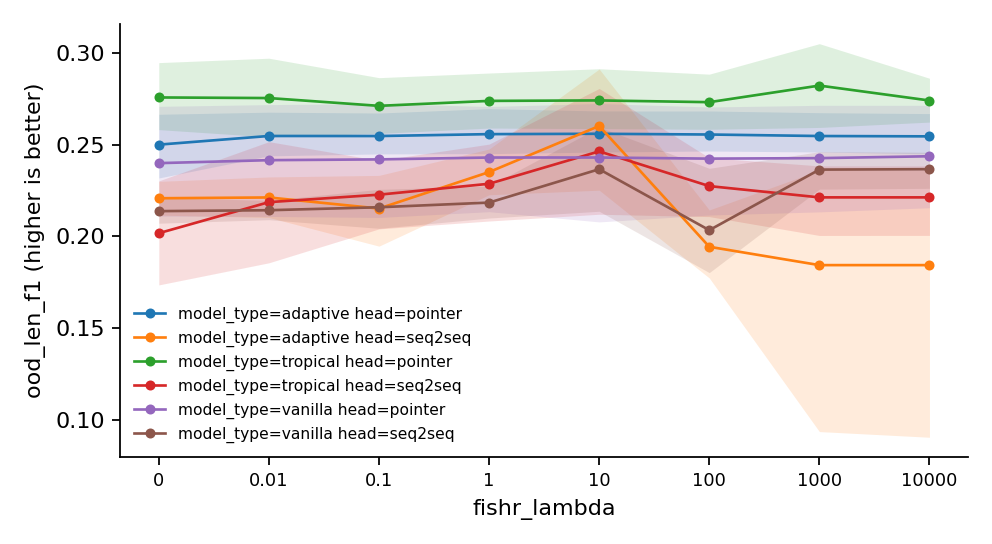
\includegraphics[width=\textwidth]{metric_ood_len_f1.png}
\caption{\texttt{ood\_len\_f1} against \texttt{fishr\_lambda}: the mean over seeds with a 95\% bootstrap CI, one line per combination of the other factors.}
\label{fig:ood_len_f1}
\end{figure}

{\small
\begin{longtable}{lllrlrrr}
\caption{\texttt{ood\_len\_f1} per cell: mean, 95\% bootstrap CI, SD, seeds, diverged runs.}\label{tab:summary-ood_len_f1}\\
\toprule
\texttt{model\_type} & \texttt{head} & \texttt{fishr\_lambda} & mean & 95\% CI & SD & $n$ & div.\\
\midrule
\endhead
adaptive & pointer & 0 & 0.25 & [0.232, 0.267] & 0.0208 & 5 & 0\\
adaptive & pointer & 0.01 & 0.2547 & [0.244, 0.268] & 0.0149 & 5 & 0\\
adaptive & pointer & 0.1 & 0.2547 & [0.245, 0.267] & 0.0151 & 5 & 0\\
adaptive & pointer & 1 & 0.2557 & [0.245, 0.27] & 0.0152 & 5 & 0\\
adaptive & pointer & 10 & 0.2559 & [0.246, 0.268] & 0.0148 & 5 & 0\\
adaptive & pointer & 100 & 0.2555 & [0.247, 0.268] & 0.0145 & 5 & 0\\
adaptive & pointer & 1000 & 0.2547 & [0.246, 0.267] & 0.0143 & 5 & 0\\
adaptive & pointer & 1e+04 & 0.2545 & [0.245, 0.267] & 0.0137 & 5 & 0\\
adaptive & seq2seq & 0 & 0.2208 & [0.212, 0.23] & 0.0119 & 5 & 0\\
adaptive & seq2seq & 0.01 & 0.2212 & [0.21, 0.232] & 0.0146 & 5 & 0\\
adaptive & seq2seq & 0.1 & 0.2152 & [0.195, 0.233] & 0.0238 & 5 & 0\\
adaptive & seq2seq & 1 & 0.235 & [0.223, 0.248] & 0.0162 & 5 & 0\\
adaptive & seq2seq & 10 & 0.2602 & [0.225, 0.291] & 0.0444 & 5 & 0\\
adaptive & seq2seq & 100 & 0.1943 & [0.177, 0.214] & 0.0244 & 5 & 0\\
adaptive & seq2seq & 1000 & 0.1843 & [0.0935, 0.236] & 0.103 & 5 & 0\\
adaptive & seq2seq & 1e+04 & 0.1843 & [0.0904, 0.236] & 0.103 & 5 & 0\\
tropical & pointer & 0 & 0.2757 & [0.258, 0.295] & 0.0239 & 5 & 0\\
tropical & pointer & 0.01 & 0.2754 & [0.254, 0.297] & 0.0279 & 5 & 0\\
tropical & pointer & 0.1 & 0.2711 & [0.256, 0.287] & 0.0201 & 5 & 0\\
tropical & pointer & 1 & 0.2739 & [0.259, 0.289] & 0.02 & 5 & 0\\
tropical & pointer & 10 & 0.2741 & [0.259, 0.291] & 0.0214 & 5 & 0\\
tropical & pointer & 100 & 0.2732 & [0.258, 0.288] & 0.0191 & 5 & 0\\
tropical & pointer & 1000 & 0.2822 & [0.259, 0.305] & 0.0298 & 5 & 0\\
tropical & pointer & 1e+04 & 0.2741 & [0.262, 0.286] & 0.0161 & 5 & 0\\
tropical & seq2seq & 0 & 0.2017 & [0.174, 0.23] & 0.0375 & 5 & 0\\
tropical & seq2seq & 0.01 & 0.2186 & [0.186, 0.252] & 0.0419 & 5 & 0\\
tropical & seq2seq & 0.1 & 0.2227 & [0.204, 0.241] & 0.0236 & 5 & 0\\
tropical & seq2seq & 1 & 0.2287 & [0.208, 0.25] & 0.0288 & 5 & 0\\
tropical & seq2seq & 10 & 0.2463 & [0.212, 0.281] & 0.044 & 5 & 0\\
tropical & seq2seq & 100 & 0.2274 & [0.211, 0.243] & 0.0216 & 5 & 0\\
tropical & seq2seq & 1000 & 0.2212 & [0.2, 0.238] & 0.0254 & 5 & 0\\
tropical & seq2seq & 1e+04 & 0.2212 & [0.201, 0.238] & 0.0254 & 5 & 0\\
vanilla & pointer & 0 & 0.2399 & [0.211, 0.271] & 0.039 & 5 & 0\\
vanilla & pointer & 0.01 & 0.2415 & [0.211, 0.272] & 0.0395 & 5 & 0\\
vanilla & pointer & 0.1 & 0.242 & [0.21, 0.272] & 0.04 & 5 & 0\\
vanilla & pointer & 1 & 0.243 & [0.213, 0.271] & 0.0384 & 5 & 0\\
vanilla & pointer & 10 & 0.243 & [0.208, 0.272] & 0.0389 & 5 & 0\\
vanilla & pointer & 100 & 0.2424 & [0.212, 0.271] & 0.0394 & 5 & 0\\
vanilla & pointer & 1000 & 0.2426 & [0.213, 0.271] & 0.0378 & 5 & 0\\
vanilla & pointer & 1e+04 & 0.2437 & [0.216, 0.271] & 0.0366 & 5 & 0\\
vanilla & seq2seq & 0 & 0.2137 & [0.207, 0.221] & 0.00898 & 5 & 0\\
vanilla & seq2seq & 0.01 & 0.2142 & [0.209, 0.22] & 0.00708 & 5 & 0\\
vanilla & seq2seq & 0.1 & 0.2159 & [0.204, 0.226] & 0.0137 & 5 & 0\\
vanilla & seq2seq & 1 & 0.2184 & [0.21, 0.227] & 0.0114 & 5 & 0\\
vanilla & seq2seq & 10 & 0.2366 & [0.214, 0.26] & 0.0289 & 5 & 0\\
vanilla & seq2seq & 100 & 0.2034 & [0.18, 0.237] & 0.0366 & 5 & 0\\
vanilla & seq2seq & 1000 & 0.2364 & [0.226, 0.246] & 0.0133 & 5 & 0\\
vanilla & seq2seq & 1e+04 & 0.2366 & [0.226, 0.246] & 0.0132 & 5 & 0\\
\bottomrule
\end{longtable}
}

{\small
\begin{longtable}{lllrrrl}
\caption{\texttt{ood\_len\_f1}: each level of \texttt{fishr\_lambda} against its control (0), within each combination of the other factors. parametric: Dunnett vs control.}\label{tab:control-ood_len_f1}\\
\toprule
\texttt{model\_type} & \texttt{head} & \texttt{fishr\_lambda} & difference & 95\% CI & $p$ & \\
\midrule
\endhead
adaptive & pointer & 0.01 & 0.004722 & [-0.0224, 0.0319] & 0.9964 & \\
adaptive & pointer & 0.1 & 0.004689 & [-0.0225, 0.0319] & 0.9965 & \\
adaptive & pointer & 1 & 0.005729 & [-0.0214, 0.0329] & 0.9889 & \\
adaptive & pointer & 10 & 0.005918 & [-0.0212, 0.0331] & 0.9867 & \\
adaptive & pointer & 100 & 0.005523 & [-0.0216, 0.0327] & 0.9909 & \\
adaptive & pointer & 1000 & 0.004699 & [-0.0225, 0.0319] & 0.9965 & \\
adaptive & pointer & 1e+04 & 0.004518 & [-0.0226, 0.0317] & 0.9972 & \\
adaptive & seq2seq & 0.01 & $4.315\times10^{-4}$ & [-0.0975, 0.0984] & 1.0000 & \\
adaptive & seq2seq & 0.1 & -0.005603 & [-0.104, 0.0923] & 1.0000 & \\
adaptive & seq2seq & 1 & 0.01428 & [-0.0837, 0.112] & 0.9988 & \\
adaptive & seq2seq & 10 & 0.03939 & [-0.0585, 0.137] & 0.7880 & \\
adaptive & seq2seq & 100 & -0.02646 & [-0.124, 0.0715] & 0.9592 & \\
adaptive & seq2seq & 1000 & -0.03646 & [-0.134, 0.0615] & 0.8385 & \\
adaptive & seq2seq & 1e+04 & -0.03646 & [-0.134, 0.0615] & 0.8386 & \\
tropical & pointer & 0.01 & $-3.323\times10^{-4}$ & [-0.04, 0.0394] & 1.0000 & \\
tropical & pointer & 0.1 & -0.004586 & [-0.0443, 0.0351] & 0.9997 & \\
tropical & pointer & 1 & -0.001881 & [-0.0416, 0.0378] & 1.0000 & \\
tropical & pointer & 10 & -0.001621 & [-0.0413, 0.0381] & 1.0000 & \\
tropical & pointer & 100 & -0.002576 & [-0.0423, 0.0371] & 1.0000 & \\
tropical & pointer & 1000 & 0.006478 & [-0.0332, 0.0462] & 0.9975 & \\
tropical & pointer & 1e+04 & -0.001668 & [-0.0414, 0.038] & 1.0000 & \\
tropical & seq2seq & 0.01 & 0.01693 & [-0.0391, 0.073] & 0.9313 & \\
tropical & seq2seq & 0.1 & 0.021 & [-0.0351, 0.0771] & 0.8350 & \\
tropical & seq2seq & 1 & 0.02696 & [-0.0291, 0.083] & 0.6390 & \\
tropical & seq2seq & 10 & 0.04463 & [-0.0114, 0.101] & 0.1644 & \\
tropical & seq2seq & 100 & 0.02569 & [-0.0304, 0.0818] & 0.6833 & \\
tropical & seq2seq & 1000 & 0.01954 & [-0.0365, 0.0756] & 0.8746 & \\
tropical & seq2seq & 1e+04 & 0.01954 & [-0.0365, 0.0756] & 0.8746 & \\
vanilla & pointer & 0.01 & 0.001619 & [-0.066, 0.0693] & 1.0000 & \\
vanilla & pointer & 0.1 & 0.002041 & [-0.0656, 0.0697] & 1.0000 & \\
vanilla & pointer & 1 & 0.003061 & [-0.0646, 0.0707] & 1.0000 & \\
vanilla & pointer & 10 & 0.003066 & [-0.0646, 0.0707] & 1.0000 & \\
vanilla & pointer & 100 & 0.002457 & [-0.0652, 0.0701] & 1.0000 & \\
vanilla & pointer & 1000 & 0.00273 & [-0.0649, 0.0704] & 1.0000 & \\
vanilla & pointer & 1e+04 & 0.003753 & [-0.0639, 0.0714] & 1.0000 & \\
vanilla & seq2seq & 0.01 & $5.051\times10^{-4}$ & [-0.0332, 0.0342] & 1.0000 & \\
vanilla & seq2seq & 0.1 & 0.002118 & [-0.0316, 0.0358] & 1.0000 & \\
vanilla & seq2seq & 1 & 0.004662 & [-0.029, 0.0384] & 0.9991 & \\
vanilla & seq2seq & 10 & 0.02287 & [-0.0108, 0.0566] & 0.2952 & \\
vanilla & seq2seq & 100 & -0.01038 & [-0.0441, 0.0233] & 0.9252 & \\
vanilla & seq2seq & 1000 & 0.02265 & [-0.0111, 0.0564] & 0.3041 & \\
vanilla & seq2seq & 1e+04 & 0.02287 & [-0.0108, 0.0566] & 0.2948 & \\
\bottomrule
\end{longtable}
}

{\small
\begin{longtable}{llrrrrr}
\caption{\texttt{ood\_len\_f1} against log10 \texttt{fishr\_lambda}: parametric: OLS slope t-test, seed-bootstrap CI, with the Jonckheere--Terpstra ordered-trend $\tau$ and $p$.}\label{tab:trend-ood_len_f1}\\
\toprule
\texttt{model\_type} & \texttt{head} & estimate & 95\% CI & $p$ & JT $\tau$ & JT $p$\\
\midrule
\endhead
adaptive & pointer & $-2.855\times10^{-5}$ & [$-3.83\times10^{-4}$, $2.89\times10^{-4}$] & 0.9802 & -0.0552 & 0.6755\\
adaptive & seq2seq & -0.007612 & [-0.0244, 0.00398] & 0.1379 & -0.0305 & 0.8214\\
tropical & pointer & $6.223\times10^{-4}$ & [$-3.40\times10^{-5}$, 0.00128] & 0.7281 & 0.101 & 0.4661\\
tropical & seq2seq & $1.287\times10^{-4}$ & [-0.00533, 0.00559] & 0.9600 & 0.0114 & 0.9380\\
vanilla & pointer & $2.562\times10^{-4}$ & [$-1.35\times10^{-4}$, $6.13\times10^{-4}$] & 0.9327 & 0.0324 & 0.8278\\
vanilla & seq2seq & 0.003326 & [$9.08\times10^{-4}$, 0.006] & 0.0781 & 0.246 & 0.0602\\
\bottomrule
\end{longtable}
}

{\small
\begin{longtable}{lrrrl}
\caption{\texttt{ood\_len\_f1}: paired contrasts by seed, Holm-corrected across the cells. parametric: paired t-test by seed, Holm.}\label{tab:paired-ood_len_f1}\\
\toprule
contrast (within) & difference & 95\% CI & $p$ & \\
\midrule
\endhead
\stackcell{model\_type: tropical - vanilla\\\footnotesize head=pointer fishr\_lambda=0 } & 0.03582 & [-0.0177, 0.0894] & 1.0000 & \\
\stackcell{model\_type: tropical - vanilla\\\footnotesize head=pointer fishr\_lambda=0.01 } & 0.03387 & [-0.0354, 0.103] & 1.0000 & \\
\stackcell{model\_type: tropical - vanilla\\\footnotesize head=pointer fishr\_lambda=0.1 } & 0.0292 & [-0.0331, 0.0915] & 1.0000 & \\
\stackcell{model\_type: tropical - vanilla\\\footnotesize head=pointer fishr\_lambda=1 } & 0.03088 & [-0.0271, 0.0889] & 1.0000 & \\
\stackcell{model\_type: tropical - vanilla\\\footnotesize head=pointer fishr\_lambda=10 } & 0.03113 & [-0.0352, 0.0975] & 1.0000 & \\
\stackcell{model\_type: tropical - vanilla\\\footnotesize head=pointer fishr\_lambda=100 } & 0.03079 & [-0.0298, 0.0914] & 1.0000 & \\
\stackcell{model\_type: tropical - vanilla\\\footnotesize head=pointer fishr\_lambda=1000 } & 0.03957 & [-0.0277, 0.107] & 1.0000 & \\
\stackcell{model\_type: tropical - vanilla\\\footnotesize head=pointer fishr\_lambda=1e+04 } & 0.0304 & [-0.0267, 0.0875] & 1.0000 & \\
\stackcell{model\_type: tropical - vanilla\\\footnotesize head=seq2seq fishr\_lambda=0 } & -0.01203 & [-0.0662, 0.0421] & 1.0000 & \\
\stackcell{model\_type: tropical - vanilla\\\footnotesize head=seq2seq fishr\_lambda=0.01 } & 0.004399 & [-0.0507, 0.0595] & 1.0000 & \\
\stackcell{model\_type: tropical - vanilla\\\footnotesize head=seq2seq fishr\_lambda=0.1 } & 0.006853 & [-0.0306, 0.0444] & 1.0000 & \\
\stackcell{model\_type: tropical - vanilla\\\footnotesize head=seq2seq fishr\_lambda=1 } & 0.01027 & [-0.0146, 0.0352] & 1.0000 & \\
\stackcell{model\_type: tropical - vanilla\\\footnotesize head=seq2seq fishr\_lambda=10 } & 0.009735 & [-0.0413, 0.0608] & 1.0000 & \\
\stackcell{model\_type: tropical - vanilla\\\footnotesize head=seq2seq fishr\_lambda=100 } & 0.02403 & [-0.0445, 0.0926] & 1.0000 & \\
\stackcell{model\_type: tropical - vanilla\\\footnotesize head=seq2seq fishr\_lambda=1000 } & -0.01514 & [-0.0484, 0.0182] & 1.0000 & \\
\stackcell{model\_type: tropical - vanilla\\\footnotesize head=seq2seq fishr\_lambda=1e+04 } & -0.01537 & [-0.0486, 0.0178] & 1.0000 & \\
\stackcell{model\_type: adaptive - vanilla\\\footnotesize head=pointer fishr\_lambda=0 } & 0.01009 & [-0.0227, 0.0429] & 1.0000 & \\
\stackcell{model\_type: adaptive - vanilla\\\footnotesize head=pointer fishr\_lambda=0.01 } & 0.01319 & [-0.0367, 0.0631] & 1.0000 & \\
\stackcell{model\_type: adaptive - vanilla\\\footnotesize head=pointer fishr\_lambda=0.1 } & 0.01274 & [-0.0377, 0.0632] & 1.0000 & \\
\stackcell{model\_type: adaptive - vanilla\\\footnotesize head=pointer fishr\_lambda=1 } & 0.01276 & [-0.0356, 0.0611] & 1.0000 & \\
\stackcell{model\_type: adaptive - vanilla\\\footnotesize head=pointer fishr\_lambda=10 } & 0.01294 & [-0.0373, 0.0632] & 1.0000 & \\
\stackcell{model\_type: adaptive - vanilla\\\footnotesize head=pointer fishr\_lambda=100 } & 0.01315 & [-0.0357, 0.062] & 1.0000 & \\
\stackcell{model\_type: adaptive - vanilla\\\footnotesize head=pointer fishr\_lambda=1000 } & 0.01206 & [-0.034, 0.0581] & 1.0000 & \\
\stackcell{model\_type: adaptive - vanilla\\\footnotesize head=pointer fishr\_lambda=1e+04 } & 0.01085 & [-0.0351, 0.0568] & 1.0000 & \\
\stackcell{model\_type: adaptive - vanilla\\\footnotesize head=seq2seq fishr\_lambda=0 } & 0.007029 & [-0.00837, 0.0224] & 1.0000 & \\
\stackcell{model\_type: adaptive - vanilla\\\footnotesize head=seq2seq fishr\_lambda=0.01 } & 0.006955 & [-0.00667, 0.0206] & 1.0000 & \\
\stackcell{model\_type: adaptive - vanilla\\\footnotesize head=seq2seq fishr\_lambda=0.1 } & $-6.922\times10^{-4}$ & [-0.0338, 0.0324] & 1.0000 & \\
\stackcell{model\_type: adaptive - vanilla\\\footnotesize head=seq2seq fishr\_lambda=1 } & 0.01664 & [-0.0047, 0.038] & 1.0000 & \\
\stackcell{model\_type: adaptive - vanilla\\\footnotesize head=seq2seq fishr\_lambda=10 } & 0.02355 & [-0.0389, 0.086] & 1.0000 & \\
\stackcell{model\_type: adaptive - vanilla\\\footnotesize head=seq2seq fishr\_lambda=100 } & -0.009058 & [-0.0748, 0.0567] & 1.0000 & \\
\stackcell{model\_type: adaptive - vanilla\\\footnotesize head=seq2seq fishr\_lambda=1000 } & -0.05208 & [-0.178, 0.0743] & 1.0000 & \\
\stackcell{model\_type: adaptive - vanilla\\\footnotesize head=seq2seq fishr\_lambda=1e+04 } & -0.05231 & [-0.179, 0.0747] & 1.0000 & \\
\stackcell{head: pointer - seq2seq\\\footnotesize model\_type=adaptive fishr\_lambda=0 } & 0.02923 & [0.00157, 0.0569] & 0.7348 & \\
\stackcell{head: pointer - seq2seq\\\footnotesize model\_type=adaptive fishr\_lambda=0.01 } & 0.03352 & [0.00705, 0.06] & 0.5156 & \\
\stackcell{head: pointer - seq2seq\\\footnotesize model\_type=adaptive fishr\_lambda=0.1 } & 0.03953 & [0.00895, 0.0701] & 0.5056 & \\
\stackcell{head: pointer - seq2seq\\\footnotesize model\_type=adaptive fishr\_lambda=1 } & 0.02069 & [-0.0118, 0.0532] & 1.0000 & \\
\stackcell{head: pointer - seq2seq\\\footnotesize model\_type=adaptive fishr\_lambda=10 } & -0.00424 & [-0.0603, 0.0518] & 1.0000 & \\
\stackcell{head: pointer - seq2seq\\\footnotesize model\_type=adaptive fishr\_lambda=100 } & 0.06122 & [0.0305, 0.092] & 0.1258 & \\
\stackcell{head: pointer - seq2seq\\\footnotesize model\_type=adaptive fishr\_lambda=1000 } & 0.07039 & [-0.051, 0.192] & 1.0000 & \\
\stackcell{head: pointer - seq2seq\\\footnotesize model\_type=adaptive fishr\_lambda=1e+04 } & 0.07021 & [-0.0488, 0.189] & 1.0000 & \\
\stackcell{head: pointer - seq2seq\\\footnotesize model\_type=tropical fishr\_lambda=0 } & 0.07403 & [0.00205, 0.146] & 0.7348 & \\
\stackcell{head: pointer - seq2seq\\\footnotesize model\_type=tropical fishr\_lambda=0.01 } & 0.05676 & [0.00206, 0.111] & 0.7348 & \\
\stackcell{head: pointer - seq2seq\\\footnotesize model\_type=tropical fishr\_lambda=0.1 } & 0.04844 & [0.0147, 0.0822] & 0.3765 & \\
\stackcell{head: pointer - seq2seq\\\footnotesize model\_type=tropical fishr\_lambda=1 } & 0.04519 & [0.00787, 0.0825] & 0.5367 & \\
\stackcell{head: pointer - seq2seq\\\footnotesize model\_type=tropical fishr\_lambda=10 } & 0.02777 & [-0.0378, 0.0934] & 1.0000 & \\
\stackcell{head: pointer - seq2seq\\\footnotesize model\_type=tropical fishr\_lambda=100 } & 0.04576 & [0.00868, 0.0828] & 0.5324 & \\
\stackcell{head: pointer - seq2seq\\\footnotesize model\_type=tropical fishr\_lambda=1000 } & 0.06097 & [$-9.64\times10^{-4}$, 0.123] & 0.7348 & \\
\stackcell{head: pointer - seq2seq\\\footnotesize model\_type=tropical fishr\_lambda=1e+04 } & 0.05282 & [0.00357, 0.102] & 0.7348 & \\
\stackcell{head: pointer - seq2seq\\\footnotesize model\_type=vanilla fishr\_lambda=0 } & 0.02617 & [-0.0319, 0.0843] & 1.0000 & \\
\stackcell{head: pointer - seq2seq\\\footnotesize model\_type=vanilla fishr\_lambda=0.01 } & 0.02729 & [-0.0257, 0.0803] & 1.0000 & \\
\stackcell{head: pointer - seq2seq\\\footnotesize model\_type=vanilla fishr\_lambda=0.1 } & 0.0261 & [-0.0267, 0.0789] & 1.0000 & \\
\stackcell{head: pointer - seq2seq\\\footnotesize model\_type=vanilla fishr\_lambda=1 } & 0.02457 & [-0.0245, 0.0736] & 1.0000 & \\
\stackcell{head: pointer - seq2seq\\\footnotesize model\_type=vanilla fishr\_lambda=10 } & 0.006374 & [-0.074, 0.0867] & 1.0000 & \\
\stackcell{head: pointer - seq2seq\\\footnotesize model\_type=vanilla fishr\_lambda=100 } & 0.03901 & [-0.00397, 0.082] & 0.8496 & \\
\stackcell{head: pointer - seq2seq\\\footnotesize model\_type=vanilla fishr\_lambda=1000 } & 0.006255 & [-0.0446, 0.0571] & 1.0000 & \\
\stackcell{head: pointer - seq2seq\\\footnotesize model\_type=vanilla fishr\_lambda=1e+04 } & 0.007053 & [-0.0423, 0.0564] & 1.0000 & \\
\bottomrule
\end{longtable}
}

\clearpage
\appendix
\section{Other metrics}
\subsection{\texttt{ood\_len\_exact}}
\begin{figure}[tbp]
\centering
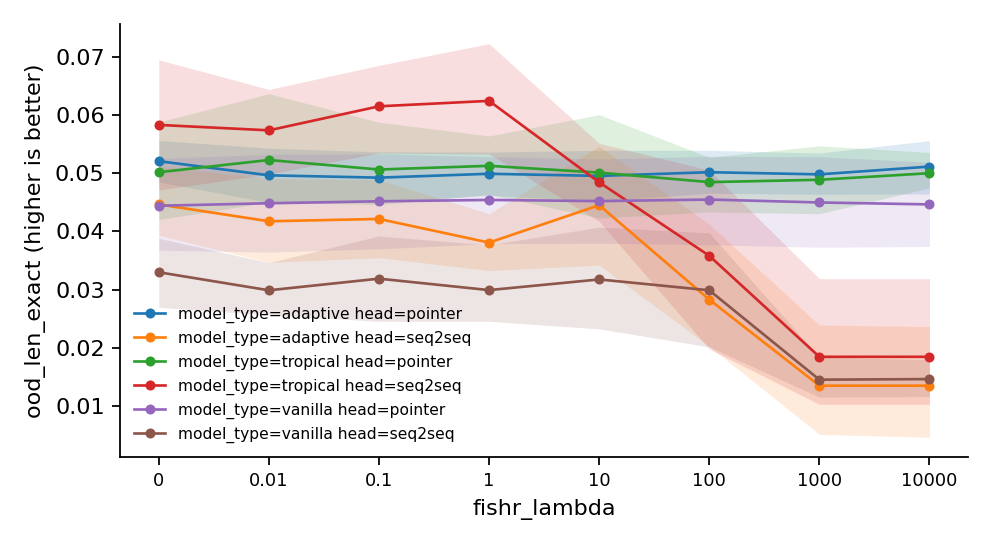
\includegraphics[width=\textwidth]{metric_ood_len_exact.png}
\caption{\texttt{ood\_len\_exact} against \texttt{fishr\_lambda}: the mean over seeds with a 95\% bootstrap CI, one line per combination of the other factors.}
\label{fig:ood_len_exact}
\end{figure}

{\small
\begin{longtable}{lllrlrrr}
\caption{\texttt{ood\_len\_exact} per cell: mean, 95\% bootstrap CI, SD, seeds, diverged runs.}\label{tab:summary-ood_len_exact}\\
\toprule
\texttt{model\_type} & \texttt{head} & \texttt{fishr\_lambda} & mean & 95\% CI & SD & $n$ & div.\\
\midrule
\endhead
adaptive & pointer & 0 & 0.05207 & [0.0485, 0.0556] & 0.00491 & 5 & 0\\
adaptive & pointer & 0.01 & 0.04963 & [0.045, 0.0543] & 0.00595 & 5 & 0\\
adaptive & pointer & 0.1 & 0.04923 & [0.045, 0.0537] & 0.00555 & 5 & 0\\
adaptive & pointer & 1 & 0.0499 & [0.0462, 0.0536] & 0.00485 & 5 & 0\\
adaptive & pointer & 10 & 0.04953 & [0.0453, 0.0539] & 0.00569 & 5 & 0\\
adaptive & pointer & 100 & 0.05017 & [0.0465, 0.0539] & 0.00485 & 5 & 0\\
adaptive & pointer & 1000 & 0.0498 & [0.0464, 0.0535] & 0.00455 & 5 & 0\\
adaptive & pointer & 1e+04 & 0.05113 & [0.0464, 0.0556] & 0.00608 & 5 & 0\\
adaptive & seq2seq & 0 & 0.04463 & [0.0393, 0.0512] & 0.00756 & 5 & 0\\
adaptive & seq2seq & 0.01 & 0.04173 & [0.0347, 0.0491] & 0.00973 & 5 & 0\\
adaptive & seq2seq & 0.1 & 0.04213 & [0.0355, 0.0489] & 0.0088 & 5 & 0\\
adaptive & seq2seq & 1 & 0.03807 & [0.0333, 0.043] & 0.00674 & 5 & 0\\
adaptive & seq2seq & 10 & 0.0445 & [0.0342, 0.0546] & 0.0133 & 5 & 0\\
adaptive & seq2seq & 100 & 0.02827 & [0.0202, 0.0412] & 0.0145 & 5 & 0\\
adaptive & seq2seq & 1000 & 0.01347 & [0.0051, 0.0239] & 0.0124 & 5 & 0\\
adaptive & seq2seq & 1e+04 & 0.01347 & [0.0046, 0.0236] & 0.0124 & 5 & 0\\
tropical & pointer & 0 & 0.05017 & [0.042, 0.0588] & 0.0112 & 5 & 0\\
tropical & pointer & 0.01 & 0.05227 & [0.045, 0.0637] & 0.0127 & 5 & 0\\
tropical & pointer & 0.1 & 0.05063 & [0.0446, 0.0588] & 0.00968 & 5 & 0\\
tropical & pointer & 1 & 0.05127 & [0.0463, 0.0564] & 0.00655 & 5 & 0\\
tropical & pointer & 10 & 0.0501 & [0.0423, 0.0601] & 0.0114 & 5 & 0\\
tropical & pointer & 100 & 0.04847 & [0.0433, 0.0527] & 0.00627 & 5 & 0\\
tropical & pointer & 1000 & 0.04887 & [0.043, 0.0547] & 0.00754 & 5 & 0\\
tropical & pointer & 1e+04 & 0.05 & [0.0475, 0.0536] & 0.00394 & 5 & 0\\
tropical & seq2seq & 0 & 0.0583 & [0.0471, 0.0695] & 0.0147 & 5 & 0\\
tropical & seq2seq & 0.01 & 0.05737 & [0.0498, 0.0644] & 0.00993 & 5 & 0\\
tropical & seq2seq & 0.1 & 0.0615 & [0.0535, 0.0685] & 0.00987 & 5 & 0\\
tropical & seq2seq & 1 & 0.06243 & [0.0533, 0.0723] & 0.0125 & 5 & 0\\
tropical & seq2seq & 10 & 0.04843 & [0.0417, 0.0551] & 0.00906 & 5 & 0\\
tropical & seq2seq & 100 & 0.0358 & [0.0198, 0.0505] & 0.0202 & 5 & 0\\
tropical & seq2seq & 1000 & 0.01843 & [0.0103, 0.0319] & 0.015 & 5 & 0\\
tropical & seq2seq & 1e+04 & 0.01843 & [0.0103, 0.0319] & 0.015 & 5 & 0\\
vanilla & pointer & 0 & 0.0444 & [0.0368, 0.0525] & 0.0103 & 5 & 0\\
vanilla & pointer & 0.01 & 0.04483 & [0.0364, 0.0532] & 0.0108 & 5 & 0\\
vanilla & pointer & 0.1 & 0.04517 & [0.037, 0.0533] & 0.0105 & 5 & 0\\
vanilla & pointer & 1 & 0.0454 & [0.0379, 0.0528] & 0.00964 & 5 & 0\\
vanilla & pointer & 10 & 0.0452 & [0.038, 0.0524] & 0.00924 & 5 & 0\\
vanilla & pointer & 100 & 0.04547 & [0.0377, 0.0529] & 0.01 & 5 & 0\\
vanilla & pointer & 1000 & 0.04497 & [0.0373, 0.0528] & 0.0101 & 5 & 0\\
vanilla & pointer & 1e+04 & 0.04463 & [0.0374, 0.0519] & 0.00921 & 5 & 0\\
vanilla & seq2seq & 0 & 0.03297 & [0.0269, 0.0388] & 0.00779 & 5 & 0\\
vanilla & seq2seq & 0.01 & 0.02987 & [0.0256, 0.0346] & 0.00571 & 5 & 0\\
vanilla & seq2seq & 0.1 & 0.03187 & [0.0245, 0.0392] & 0.00981 & 5 & 0\\
vanilla & seq2seq & 1 & 0.0299 & [0.0245, 0.0377] & 0.00879 & 5 & 0\\
vanilla & seq2seq & 10 & 0.03173 & [0.0232, 0.0407] & 0.0119 & 5 & 0\\
vanilla & seq2seq & 100 & 0.02987 & [0.0201, 0.0397] & 0.0127 & 5 & 0\\
vanilla & seq2seq & 1000 & 0.0145 & [0.0115, 0.0184] & 0.00429 & 5 & 0\\
vanilla & seq2seq & 1e+04 & 0.0146 & [0.0116, 0.0179] & 0.00424 & 5 & 0\\
\bottomrule
\end{longtable}
}

{\small
\begin{longtable}{lllrrrl}
\caption{\texttt{ood\_len\_exact}: each level of \texttt{fishr\_lambda} against its control (0), within each combination of the other factors. parametric: Dunnett vs control.}\label{tab:control-ood_len_exact}\\
\toprule
\texttt{model\_type} & \texttt{head} & \texttt{fishr\_lambda} & difference & 95\% CI & $p$ & \\
\midrule
\endhead
adaptive & pointer & 0.01 & -0.002433 & [-0.0117, 0.00688] & 0.9654 & \\
adaptive & pointer & 0.1 & -0.002833 & [-0.0121, 0.00648] & 0.9291 & \\
adaptive & pointer & 1 & -0.002167 & [-0.0115, 0.00715] & 0.9810 & \\
adaptive & pointer & 10 & -0.002533 & [-0.0118, 0.00678] & 0.9579 & \\
adaptive & pointer & 100 & -0.0019 & [-0.0112, 0.00741] & 0.9907 & \\
adaptive & pointer & 1000 & -0.002267 & [-0.0116, 0.00705] & 0.9759 & \\
adaptive & pointer & 1e+04 & $-9.333\times10^{-4}$ & [-0.0102, 0.00838] & 0.9999 & \\
adaptive & seq2seq & 0.01 & -0.0029 & [-0.0221, 0.0163] & 0.9985 & \\
adaptive & seq2seq & 0.1 & -0.0025 & [-0.0217, 0.0167] & 0.9994 & \\
adaptive & seq2seq & 1 & -0.006567 & [-0.0258, 0.0127] & 0.8842 & \\
adaptive & seq2seq & 10 & $-1.333\times10^{-4}$ & [-0.0194, 0.0191] & 1.0000 & \\
adaptive & seq2seq & 100 & -0.01637 & [-0.0356, 0.00286] & 0.1216 & \\
adaptive & seq2seq & 1000 & -0.03117 & [-0.0504, -0.0119] & 0.0006 & *\\
adaptive & seq2seq & 1e+04 & -0.03117 & [-0.0504, -0.0119] & 0.0006 & *\\
tropical & pointer & 0.01 & 0.0021 & [-0.0138, 0.018] & 0.9993 & \\
tropical & pointer & 0.1 & $4.667\times10^{-4}$ & [-0.0154, 0.0164] & 1.0000 & \\
tropical & pointer & 1 & 0.0011 & [-0.0148, 0.017] & 1.0000 & \\
tropical & pointer & 10 & $-6.667\times10^{-5}$ & [-0.016, 0.0158] & 1.0000 & \\
tropical & pointer & 100 & -0.0017 & [-0.0176, 0.0142] & 0.9998 & \\
tropical & pointer & 1000 & -0.0013 & [-0.0172, 0.0146] & 1.0000 & \\
tropical & pointer & 1e+04 & $-1.667\times10^{-4}$ & [-0.0161, 0.0157] & 1.0000 & \\
tropical & seq2seq & 0.01 & $-9.333\times10^{-4}$ & [-0.0249, 0.023] & 1.0000 & \\
tropical & seq2seq & 0.1 & 0.0032 & [-0.0208, 0.0272] & 0.9993 & \\
tropical & seq2seq & 1 & 0.004133 & [-0.0198, 0.0281] & 0.9965 & \\
tropical & seq2seq & 10 & -0.009867 & [-0.0338, 0.0141] & 0.7714 & \\
tropical & seq2seq & 100 & -0.0225 & [-0.0465, 0.00148] & 0.0731 & \\
tropical & seq2seq & 1000 & -0.03987 & [-0.0638, -0.0159] & 0.0004 & *\\
tropical & seq2seq & 1e+04 & -0.03987 & [-0.0638, -0.0159] & 0.0004 & *\\
vanilla & pointer & 0.01 & $4.333\times10^{-4}$ & [-0.017, 0.0179] & 1.0000 & \\
vanilla & pointer & 0.1 & $7.667\times10^{-4}$ & [-0.0167, 0.0182] & 1.0000 & \\
vanilla & pointer & 1 & $1.000\times10^{-3}$ & [-0.0165, 0.0185] & 1.0000 & \\
vanilla & pointer & 10 & $8.000\times10^{-4}$ & [-0.0167, 0.0183] & 1.0000 & \\
vanilla & pointer & 100 & 0.001067 & [-0.0164, 0.0185] & 1.0000 & \\
vanilla & pointer & 1000 & $5.667\times10^{-4}$ & [-0.0169, 0.018] & 1.0000 & \\
vanilla & pointer & 1e+04 & $2.333\times10^{-4}$ & [-0.0172, 0.0177] & 1.0000 & \\
vanilla & seq2seq & 0.01 & -0.0031 & [-0.0183, 0.0121] & 0.9908 & \\
vanilla & seq2seq & 0.1 & -0.0011 & [-0.0163, 0.0141] & 1.0000 & \\
vanilla & seq2seq & 1 & -0.003067 & [-0.0183, 0.0121] & 0.9913 & \\
vanilla & seq2seq & 10 & -0.001233 & [-0.0164, 0.014] & 1.0000 & \\
vanilla & seq2seq & 100 & -0.0031 & [-0.0183, 0.0121] & 0.9908 & \\
vanilla & seq2seq & 1000 & -0.01847 & [-0.0337, -0.00326] & 0.0120 & *\\
vanilla & seq2seq & 1e+04 & -0.01837 & [-0.0336, -0.00316] & 0.0126 & *\\
\bottomrule
\end{longtable}
}

{\small
\begin{longtable}{llrrrrr}
\caption{\texttt{ood\_len\_exact} against log10 \texttt{fishr\_lambda}: parametric: OLS slope t-test, seed-bootstrap CI, with the Jonckheere--Terpstra ordered-trend $\tau$ and $p$.}\label{tab:trend-ood_len_exact}\\
\toprule
\texttt{model\_type} & \texttt{head} & estimate & 95\% CI & $p$ & JT $\tau$ & JT $p$\\
\midrule
\endhead
adaptive & pointer & $2.107\times10^{-4}$ & [$3.93\times10^{-5}$, $3.69\times10^{-4}$] & 0.6199 & 0.0743 & 0.5783\\
adaptive & seq2seq & -0.005426 & [-0.00672, -0.00413] & $<10^{-4}$ & -0.533 & 0.0002\\
tropical & pointer & $-4.690\times10^{-4}$ & [-0.00163, $1.75\times10^{-4}$] & 0.4988 & 0.0133 & 0.9296\\
tropical & seq2seq & -0.008199 & [-0.00929, -0.00696] & $<10^{-4}$ & -0.617 & 0.0002\\
vanilla & pointer & $-3.333\times10^{-5}$ & [$-1.71\times10^{-4}$, $1.13\times10^{-4}$] & 0.9659 & -0.021 & 0.8812\\
vanilla & seq2seq & -0.002877 & [-0.00425, -0.0015] & 0.0009 & -0.467 & 0.0006\\
\bottomrule
\end{longtable}
}

{\small
\begin{longtable}{lrrrl}
\caption{\texttt{ood\_len\_exact}: paired contrasts by seed, Holm-corrected across the cells. parametric: paired t-test by seed, Holm.}\label{tab:paired-ood_len_exact}\\
\toprule
contrast (within) & difference & 95\% CI & $p$ & \\
\midrule
\endhead
\stackcell{model\_type: tropical - vanilla\\\footnotesize head=pointer fishr\_lambda=0 } & 0.005767 & [-0.00952, 0.0211] & 1.0000 & \\
\stackcell{model\_type: tropical - vanilla\\\footnotesize head=pointer fishr\_lambda=0.01 } & 0.007433 & [-0.0173, 0.0322] & 1.0000 & \\
\stackcell{model\_type: tropical - vanilla\\\footnotesize head=pointer fishr\_lambda=0.1 } & 0.005467 & [-0.0173, 0.0282] & 1.0000 & \\
\stackcell{model\_type: tropical - vanilla\\\footnotesize head=pointer fishr\_lambda=1 } & 0.005867 & [-0.00954, 0.0213] & 1.0000 & \\
\stackcell{model\_type: tropical - vanilla\\\footnotesize head=pointer fishr\_lambda=10 } & 0.0049 & [-0.0172, 0.027] & 1.0000 & \\
\stackcell{model\_type: tropical - vanilla\\\footnotesize head=pointer fishr\_lambda=100 } & 0.003 & [-0.0156, 0.0216] & 1.0000 & \\
\stackcell{model\_type: tropical - vanilla\\\footnotesize head=pointer fishr\_lambda=1000 } & 0.0039 & [-0.0118, 0.0196] & 1.0000 & \\
\stackcell{model\_type: tropical - vanilla\\\footnotesize head=pointer fishr\_lambda=1e+04 } & 0.005367 & [-0.00944, 0.0202] & 1.0000 & \\
\stackcell{model\_type: tropical - vanilla\\\footnotesize head=seq2seq fishr\_lambda=0 } & 0.02533 & [0.00884, 0.0418] & 0.1690 & \\
\stackcell{model\_type: tropical - vanilla\\\footnotesize head=seq2seq fishr\_lambda=0.01 } & 0.0275 & [0.0129, 0.0421] & 0.1005 & \\
\stackcell{model\_type: tropical - vanilla\\\footnotesize head=seq2seq fishr\_lambda=0.1 } & 0.02963 & [0.012, 0.0473] & 0.1348 & \\
\stackcell{model\_type: tropical - vanilla\\\footnotesize head=seq2seq fishr\_lambda=1 } & 0.03253 & [0.0153, 0.0497] & 0.1005 & \\
\stackcell{model\_type: tropical - vanilla\\\footnotesize head=seq2seq fishr\_lambda=10 } & 0.0167 & [-0.00318, 0.0366] & 0.9605 & \\
\stackcell{model\_type: tropical - vanilla\\\footnotesize head=seq2seq fishr\_lambda=100 } & 0.005933 & [-0.0284, 0.0403] & 1.0000 & \\
\stackcell{model\_type: tropical - vanilla\\\footnotesize head=seq2seq fishr\_lambda=1000 } & 0.003933 & [-0.0161, 0.0239] & 1.0000 & \\
\stackcell{model\_type: tropical - vanilla\\\footnotesize head=seq2seq fishr\_lambda=1e+04 } & 0.003833 & [-0.0162, 0.0239] & 1.0000 & \\
\stackcell{model\_type: adaptive - vanilla\\\footnotesize head=pointer fishr\_lambda=0 } & 0.007667 & [-0.00733, 0.0227] & 1.0000 & \\
\stackcell{model\_type: adaptive - vanilla\\\footnotesize head=pointer fishr\_lambda=0.01 } & 0.0048 & [-0.0121, 0.0217] & 1.0000 & \\
\stackcell{model\_type: adaptive - vanilla\\\footnotesize head=pointer fishr\_lambda=0.1 } & 0.004067 & [-0.0115, 0.0196] & 1.0000 & \\
\stackcell{model\_type: adaptive - vanilla\\\footnotesize head=pointer fishr\_lambda=1 } & 0.0045 & [-0.0105, 0.0195] & 1.0000 & \\
\stackcell{model\_type: adaptive - vanilla\\\footnotesize head=pointer fishr\_lambda=10 } & 0.004333 & [-0.00992, 0.0186] & 1.0000 & \\
\stackcell{model\_type: adaptive - vanilla\\\footnotesize head=pointer fishr\_lambda=100 } & 0.0047 & [-0.0113, 0.0207] & 1.0000 & \\
\stackcell{model\_type: adaptive - vanilla\\\footnotesize head=pointer fishr\_lambda=1000 } & 0.004833 & [-0.0106, 0.0202] & 1.0000 & \\
\stackcell{model\_type: adaptive - vanilla\\\footnotesize head=pointer fishr\_lambda=1e+04 } & 0.0065 & [-0.00839, 0.0214] & 1.0000 & \\
\stackcell{model\_type: adaptive - vanilla\\\footnotesize head=seq2seq fishr\_lambda=0 } & 0.01167 & [$1.51\times10^{-5}$, 0.0233] & 0.7472 & \\
\stackcell{model\_type: adaptive - vanilla\\\footnotesize head=seq2seq fishr\_lambda=0.01 } & 0.01187 & [0.00154, 0.0222] & 0.5317 & \\
\stackcell{model\_type: adaptive - vanilla\\\footnotesize head=seq2seq fishr\_lambda=0.1 } & 0.01027 & [-0.00417, 0.0247] & 1.0000 & \\
\stackcell{model\_type: adaptive - vanilla\\\footnotesize head=seq2seq fishr\_lambda=1 } & 0.008167 & [-0.00244, 0.0188] & 1.0000 & \\
\stackcell{model\_type: adaptive - vanilla\\\footnotesize head=seq2seq fishr\_lambda=10 } & 0.01277 & [-0.00966, 0.0352] & 1.0000 & \\
\stackcell{model\_type: adaptive - vanilla\\\footnotesize head=seq2seq fishr\_lambda=100 } & -0.0016 & [-0.0217, 0.0185] & 1.0000 & \\
\stackcell{model\_type: adaptive - vanilla\\\footnotesize head=seq2seq fishr\_lambda=1000 } & -0.001033 & [-0.0191, 0.017] & 1.0000 & \\
\stackcell{model\_type: adaptive - vanilla\\\footnotesize head=seq2seq fishr\_lambda=1e+04 } & -0.001133 & [-0.0193, 0.017] & 1.0000 & \\
\stackcell{head: pointer - seq2seq\\\footnotesize model\_type=adaptive fishr\_lambda=0 } & 0.007433 & [-0.00142, 0.0163] & 0.8805 & \\
\stackcell{head: pointer - seq2seq\\\footnotesize model\_type=adaptive fishr\_lambda=0.01 } & 0.0079 & [-0.00324, 0.019] & 0.9521 & \\
\stackcell{head: pointer - seq2seq\\\footnotesize model\_type=adaptive fishr\_lambda=0.1 } & 0.0071 & [-0.00237, 0.0166] & 0.9521 & \\
\stackcell{head: pointer - seq2seq\\\footnotesize model\_type=adaptive fishr\_lambda=1 } & 0.01183 & [$7.26\times10^{-4}$, 0.0229] & 0.5493 & \\
\stackcell{head: pointer - seq2seq\\\footnotesize model\_type=adaptive fishr\_lambda=10 } & 0.005033 & [-0.00916, 0.0192] & 1.0000 & \\
\stackcell{head: pointer - seq2seq\\\footnotesize model\_type=adaptive fishr\_lambda=100 } & 0.0219 & [0.00175, 0.042] & 0.5493 & \\
\stackcell{head: pointer - seq2seq\\\footnotesize model\_type=adaptive fishr\_lambda=1000 } & 0.03633 & [0.0196, 0.0531] & 0.0793 & \\
\stackcell{head: pointer - seq2seq\\\footnotesize model\_type=adaptive fishr\_lambda=1e+04 } & 0.03767 & [0.0212, 0.0541] & 0.0722 & \\
\stackcell{head: pointer - seq2seq\\\footnotesize model\_type=tropical fishr\_lambda=0 } & -0.008133 & [-0.0322, 0.0159] & 1.0000 & \\
\stackcell{head: pointer - seq2seq\\\footnotesize model\_type=tropical fishr\_lambda=0.01 } & -0.0051 & [-0.0274, 0.0172] & 1.0000 & \\
\stackcell{head: pointer - seq2seq\\\footnotesize model\_type=tropical fishr\_lambda=0.1 } & -0.01087 & [-0.023, 0.00128] & 0.8152 & \\
\stackcell{head: pointer - seq2seq\\\footnotesize model\_type=tropical fishr\_lambda=1 } & -0.01117 & [-0.0305, 0.0082] & 0.9521 & \\
\stackcell{head: pointer - seq2seq\\\footnotesize model\_type=tropical fishr\_lambda=10 } & 0.001667 & [-0.0222, 0.0255] & 1.0000 & \\
\stackcell{head: pointer - seq2seq\\\footnotesize model\_type=tropical fishr\_lambda=100 } & 0.01267 & [-0.00607, 0.0314] & 0.9521 & \\
\stackcell{head: pointer - seq2seq\\\footnotesize model\_type=tropical fishr\_lambda=1000 } & 0.03043 & [0.00656, 0.0543] & 0.4085 & \\
\stackcell{head: pointer - seq2seq\\\footnotesize model\_type=tropical fishr\_lambda=1e+04 } & 0.03157 & [0.0119, 0.0512] & 0.2127 & \\
\stackcell{head: pointer - seq2seq\\\footnotesize model\_type=vanilla fishr\_lambda=0 } & 0.01143 & [-0.00223, 0.0251] & 0.8805 & \\
\stackcell{head: pointer - seq2seq\\\footnotesize model\_type=vanilla fishr\_lambda=0.01 } & 0.01497 & [0.00235, 0.0276] & 0.4519 & \\
\stackcell{head: pointer - seq2seq\\\footnotesize model\_type=vanilla fishr\_lambda=0.1 } & 0.0133 & [0.00264, 0.024] & 0.4115 & \\
\stackcell{head: pointer - seq2seq\\\footnotesize model\_type=vanilla fishr\_lambda=1 } & 0.0155 & [0.00498, 0.026] & 0.2693 & \\
\stackcell{head: pointer - seq2seq\\\footnotesize model\_type=vanilla fishr\_lambda=10 } & 0.01347 & [-0.00462, 0.0316] & 0.9521 & \\
\stackcell{head: pointer - seq2seq\\\footnotesize model\_type=vanilla fishr\_lambda=100 } & 0.0156 & [0.00843, 0.0228] & 0.0793 & \\
\stackcell{head: pointer - seq2seq\\\footnotesize model\_type=vanilla fishr\_lambda=1000 } & 0.03047 & [0.0171, 0.0438] & 0.0722 & \\
\stackcell{head: pointer - seq2seq\\\footnotesize model\_type=vanilla fishr\_lambda=1e+04 } & 0.03003 & [0.0182, 0.0419] & 0.0521 & \\
\bottomrule
\end{longtable}
}

\subsection{\texttt{ood\_val\_f1}}
\begin{figure}[tbp]
\centering
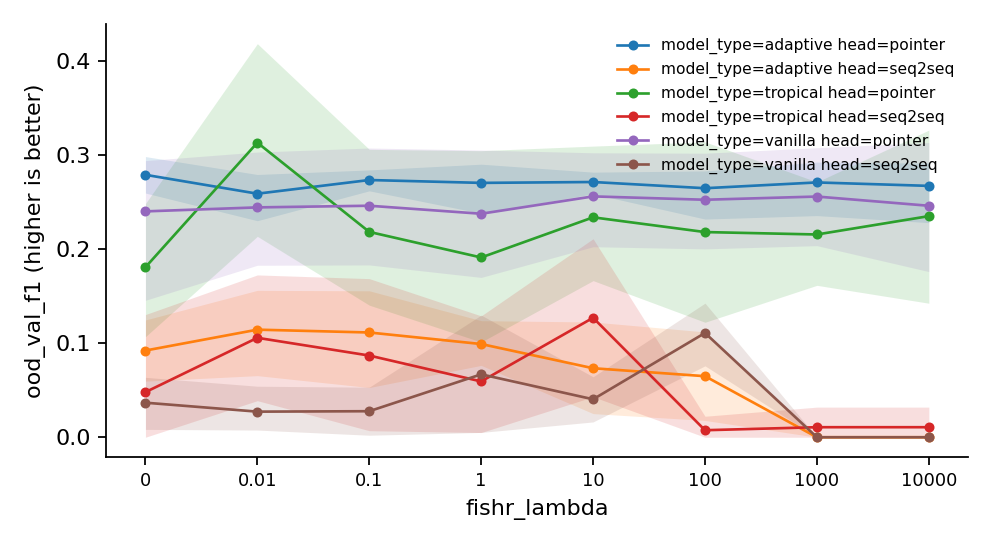
\includegraphics[width=\textwidth]{metric_ood_val_f1.png}
\caption{\texttt{ood\_val\_f1} against \texttt{fishr\_lambda}: the mean over seeds with a 95\% bootstrap CI, one line per combination of the other factors.}
\label{fig:ood_val_f1}
\end{figure}

{\small
\begin{longtable}{lllrlrrr}
\caption{\texttt{ood\_val\_f1} per cell: mean, 95\% bootstrap CI, SD, seeds, diverged runs.}\label{tab:summary-ood_val_f1}\\
\toprule
\texttt{model\_type} & \texttt{head} & \texttt{fishr\_lambda} & mean & 95\% CI & SD & $n$ & div.\\
\midrule
\endhead
adaptive & pointer & 0 & 0.279 & [0.26, 0.298] & 0.0253 & 5 & 0\\
adaptive & pointer & 0.01 & 0.2589 & [0.23, 0.279] & 0.032 & 5 & 0\\
adaptive & pointer & 0.1 & 0.2734 & [0.262, 0.284] & 0.0143 & 5 & 0\\
adaptive & pointer & 1 & 0.2704 & [0.238, 0.29] & 0.0362 & 5 & 0\\
adaptive & pointer & 10 & 0.2713 & [0.259, 0.282] & 0.0153 & 5 & 0\\
adaptive & pointer & 100 & 0.2647 & [0.232, 0.283] & 0.0367 & 5 & 0\\
adaptive & pointer & 1000 & 0.2708 & [0.236, 0.292] & 0.0384 & 5 & 0\\
adaptive & pointer & 1e+04 & 0.2672 & [0.228, 0.291] & 0.0437 & 5 & 0\\
adaptive & seq2seq & 0 & 0.09216 & [0.0596, 0.125] & 0.0435 & 5 & 0\\
adaptive & seq2seq & 0.01 & 0.1144 & [0.0655, 0.156] & 0.0594 & 5 & 0\\
adaptive & seq2seq & 0.1 & 0.1114 & [0.0528, 0.156] & 0.066 & 5 & 0\\
adaptive & seq2seq & 1 & 0.09909 & [0.0764, 0.124] & 0.0323 & 5 & 0\\
adaptive & seq2seq & 10 & 0.07335 & [0.0251, 0.123] & 0.0656 & 5 & 0\\
adaptive & seq2seq & 100 & 0.06491 & [0.0179, 0.112] & 0.059 & 5 & 0\\
adaptive & seq2seq & 1000 & 0 & [0, 0] & 0 & 5 & 0\\
adaptive & seq2seq & 1e+04 & 0 & [0, 0] & 0 & 5 & 0\\
tropical & pointer & 0 & 0.1807 & [0.107, 0.248] & 0.0907 & 5 & 0\\
tropical & pointer & 0.01 & 0.3131 & [0.214, 0.418] & 0.137 & 5 & 0\\
tropical & pointer & 0.1 & 0.2183 & [0.14, 0.306] & 0.107 & 5 & 0\\
tropical & pointer & 1 & 0.1911 & [0.101, 0.305] & 0.129 & 5 & 0\\
tropical & pointer & 10 & 0.2338 & [0.166, 0.309] & 0.0915 & 5 & 0\\
tropical & pointer & 100 & 0.2181 & [0.122, 0.314] & 0.126 & 5 & 0\\
tropical & pointer & 1000 & 0.2155 & [0.161, 0.271] & 0.0712 & 5 & 0\\
tropical & pointer & 1e+04 & 0.235 & [0.142, 0.326] & 0.12 & 5 & 0\\
tropical & seq2seq & 0 & 0.04794 & [$1.13\times10^{-5}$, 0.13] & 0.0896 & 5 & 0\\
tropical & seq2seq & 0.01 & 0.1057 & [0.0389, 0.173] & 0.0903 & 5 & 0\\
tropical & seq2seq & 0.1 & 0.08684 & [0.00696, 0.169] & 0.104 & 5 & 0\\
tropical & seq2seq & 1 & 0.05932 & [0.005, 0.129] & 0.0792 & 5 & 0\\
tropical & seq2seq & 10 & 0.127 & [0.043, 0.211] & 0.106 & 5 & 0\\
tropical & seq2seq & 100 & 0.007478 & [0, 0.0223] & 0.0166 & 5 & 0\\
tropical & seq2seq & 1000 & 0.01068 & [0, 0.032] & 0.0239 & 5 & 0\\
tropical & seq2seq & 1e+04 & 0.01068 & [0, 0.032] & 0.0239 & 5 & 0\\
vanilla & pointer & 0 & 0.2401 & [0.146, 0.294] & 0.105 & 5 & 0\\
vanilla & pointer & 0.01 & 0.2443 & [0.183, 0.303] & 0.0791 & 5 & 0\\
vanilla & pointer & 0.1 & 0.2461 & [0.183, 0.307] & 0.0815 & 5 & 0\\
vanilla & pointer & 1 & 0.2376 & [0.17, 0.305] & 0.0856 & 5 & 0\\
vanilla & pointer & 10 & 0.256 & [0.203, 0.302] & 0.0647 & 5 & 0\\
vanilla & pointer & 100 & 0.2524 & [0.2, 0.302] & 0.0681 & 5 & 0\\
vanilla & pointer & 1000 & 0.2559 & [0.204, 0.308] & 0.0685 & 5 & 0\\
vanilla & pointer & 1e+04 & 0.2461 & [0.176, 0.313] & 0.089 & 5 & 0\\
vanilla & seq2seq & 0 & 0.03673 & [0.00836, 0.0637] & 0.0356 & 5 & 0\\
vanilla & seq2seq & 0.01 & 0.02722 & [0.00763, 0.0542] & 0.0315 & 5 & 0\\
vanilla & seq2seq & 0.1 & 0.02768 & [0.00215, 0.0532] & 0.0345 & 5 & 0\\
vanilla & seq2seq & 1 & 0.06688 & [0.00514, 0.13] & 0.0832 & 5 & 0\\
vanilla & seq2seq & 10 & 0.04036 & [0.0163, 0.0643] & 0.0314 & 5 & 0\\
vanilla & seq2seq & 100 & 0.1109 & [0.0759, 0.143] & 0.0425 & 5 & 0\\
vanilla & seq2seq & 1000 & 0 & [0, 0] & 0 & 5 & 0\\
vanilla & seq2seq & 1e+04 & 0 & [0, 0] & 0 & 5 & 0\\
\bottomrule
\end{longtable}
}

{\small
\begin{longtable}{lllrrrl}
\caption{\texttt{ood\_val\_f1}: each level of \texttt{fishr\_lambda} against its control (0), within each combination of the other factors. rank: Wilcoxon signed-rank by seed, Holm.}\label{tab:control-ood_val_f1}\\
\toprule
\texttt{model\_type} & \texttt{head} & \texttt{fishr\_lambda} & difference & 95\% CI & $p$ & \\
\midrule
\endhead
adaptive & pointer & 0.01 & -0.007539 & [-0.065, 0.0106] & 1.0000 & \\
adaptive & pointer & 0.1 & 0.005768 & [-0.0316, 0.0171] & 1.0000 & \\
adaptive & pointer & 1 & 0.009014 & [-0.0575, 0.0253] & 1.0000 & \\
adaptive & pointer & 10 & 0.001851 & [-0.0365, 0.0158] & 1.0000 & \\
adaptive & pointer & 100 & -0.00694 & [-0.0635, 0.0209] & 1.0000 & \\
adaptive & pointer & 1000 & 0.008859 & [-0.0586, 0.0254] & 1.0000 & \\
adaptive & pointer & 1e+04 & $-1.281\times10^{-4}$ & [-0.0687, 0.0256] & 1.0000 & \\
adaptive & seq2seq & 0.01 & -0.0015 & [-0.0152, 0.0596] & 1.0000 & \\
adaptive & seq2seq & 0.1 & 0.02819 & [-0.0131, 0.0458] & 1.0000 & \\
adaptive & seq2seq & 1 & -0.01279 & [-0.0466, 0.0605] & 1.0000 & \\
adaptive & seq2seq & 10 & -0.009937 & [-0.0559, 0.0182] & 1.0000 & \\
adaptive & seq2seq & 100 & -0.03244 & [-0.0823, 0.0273] & 1.0000 & \\
adaptive & seq2seq & 1000 & -0.09957 & [-0.125, -0.0603] & 0.4375 & \\
adaptive & seq2seq & 1e+04 & -0.09957 & [-0.125, -0.0603] & 0.4375 & \\
tropical & pointer & 0.01 & 0.129 & [-0.00704, 0.272] & 1.0000 & \\
tropical & pointer & 0.1 & 0.0294 & [-0.0982, 0.188] & 1.0000 & \\
tropical & pointer & 1 & 0.007073 & [-0.0792, 0.0923] & 1.0000 & \\
tropical & pointer & 10 & 0.06995 & [-0.00324, 0.109] & 1.0000 & \\
tropical & pointer & 100 & 0.07303 & [-0.0522, 0.11] & 1.0000 & \\
tropical & pointer & 1000 & 0.03297 & [-0.0689, 0.148] & 1.0000 & \\
tropical & pointer & 1e+04 & 0.01755 & [-0.0449, 0.166] & 1.0000 & \\
tropical & seq2seq & 0.01 & 0.02838 & [$7.43\times10^{-4}$, 0.118] & 1.0000 & \\
tropical & seq2seq & 0.1 & 0 & [-0.0141, 0.117] & 1.0000 & \\
tropical & seq2seq & 1 & $3.262\times10^{-4}$ & [-0.067, 0.105] & 1.0000 & \\
tropical & seq2seq & 10 & 0.03551 & [0.0052, 0.158] & 1.0000 & \\
tropical & seq2seq & 100 & $-5.632\times10^{-5}$ & [-0.124, 0.0149] & 1.0000 & \\
tropical & seq2seq & 1000 & $-5.632\times10^{-5}$ & [-0.124, 0.0215] & 1.0000 & \\
tropical & seq2seq & 1e+04 & $-5.632\times10^{-5}$ & [-0.124, 0.0215] & 1.0000 & \\
vanilla & pointer & 0.01 & 0.007002 & [-0.0645, 0.0629] & 1.0000 & \\
vanilla & pointer & 0.1 & 0.008204 & [-0.0582, 0.0587] & 1.0000 & \\
vanilla & pointer & 1 & 0.01309 & [-0.0702, 0.0513] & 1.0000 & \\
vanilla & pointer & 10 & 0.0051 & [-0.0657, 0.1] & 1.0000 & \\
vanilla & pointer & 100 & 0.006125 & [-0.067, 0.091] & 1.0000 & \\
vanilla & pointer & 1000 & 0.008169 & [-0.0666, 0.0977] & 1.0000 & \\
vanilla & pointer & 1e+04 & 0.02306 & [-0.0603, 0.0566] & 1.0000 & \\
vanilla & seq2seq & 0.01 & $3.889\times10^{-4}$ & [-0.0339, 0.0149] & 1.0000 & \\
vanilla & seq2seq & 0.1 & -0.003456 & [-0.0233, $4.46\times10^{-4}$] & 1.0000 & \\
vanilla & seq2seq & 1 & 0.01133 & [-0.0114, 0.0717] & 1.0000 & \\
vanilla & seq2seq & 10 & 0.001111 & [-0.00664, 0.0147] & 1.0000 & \\
vanilla & seq2seq & 100 & 0.08463 & [0.0408, 0.107] & 0.4375 & \\
vanilla & seq2seq & 1000 & -0.04122 & [-0.0637, -0.00836] & 0.7500 & \\
vanilla & seq2seq & 1e+04 & -0.04122 & [-0.0637, -0.00836] & 0.7500 & \\
\bottomrule
\end{longtable}
}

{\small
\begin{longtable}{llrrrrr}
\caption{\texttt{ood\_val\_f1} against log10 \texttt{fishr\_lambda}: rank: Spearman rho, seed-bootstrap CI, with the Jonckheere--Terpstra ordered-trend $\tau$ and $p$.}\label{tab:trend-ood_val_f1}\\
\toprule
\texttt{model\_type} & \texttt{head} & estimate & 95\% CI & $p$ & JT $\tau$ & JT $p$\\
\midrule
\endhead
adaptive & pointer & 0.2037 & [-0.194, 0.519] & 0.2405 & 0.158 & 0.2370\\
adaptive & seq2seq & -0.7392 & [-0.862, -0.636] & $<10^{-4}$ & -0.589 & 0.0002\\
tropical & pointer & -0.1061 & [-0.478, 0.229] & 0.5442 & -0.0781 & 0.5591\\
tropical & seq2seq & -0.4387 & [-0.707, -0.165] & 0.0084 & -0.32 & 0.0096\\
vanilla & pointer & 0.03961 & [-0.156, 0.137] & 0.8213 & 0.0324 & 0.8196\\
vanilla & seq2seq & -0.4716 & [-0.542, -0.405] & 0.0042 & -0.312 & 0.0150\\
\bottomrule
\end{longtable}
}

{\small
\begin{longtable}{lrrrl}
\caption{\texttt{ood\_val\_f1}: paired contrasts by seed, Holm-corrected across the cells. rank: Wilcoxon signed-rank by seed, Holm.}\label{tab:paired-ood_val_f1}\\
\toprule
contrast (within) & difference & 95\% CI & $p$ & \\
\midrule
\endhead
\stackcell{model\_type: tropical - vanilla\\\footnotesize head=pointer fishr\_lambda=0 } & -0.05936 & [-0.271, 0.152] & 1.0000 & \\
\stackcell{model\_type: tropical - vanilla\\\footnotesize head=pointer fishr\_lambda=0.01 } & 0.06882 & [-0.156, 0.294] & 1.0000 & \\
\stackcell{model\_type: tropical - vanilla\\\footnotesize head=pointer fishr\_lambda=0.1 } & -0.02781 & [-0.172, 0.116] & 1.0000 & \\
\stackcell{model\_type: tropical - vanilla\\\footnotesize head=pointer fishr\_lambda=1 } & -0.04649 & [-0.304, 0.211] & 1.0000 & \\
\stackcell{model\_type: tropical - vanilla\\\footnotesize head=pointer fishr\_lambda=10 } & -0.02226 & [-0.21, 0.165] & 1.0000 & \\
\stackcell{model\_type: tropical - vanilla\\\footnotesize head=pointer fishr\_lambda=100 } & -0.03435 & [-0.259, 0.19] & 1.0000 & \\
\stackcell{model\_type: tropical - vanilla\\\footnotesize head=pointer fishr\_lambda=1000 } & -0.04033 & [-0.152, 0.0709] & 1.0000 & \\
\stackcell{model\_type: tropical - vanilla\\\footnotesize head=pointer fishr\_lambda=1e+04 } & -0.01102 & [-0.217, 0.195] & 1.0000 & \\
\stackcell{model\_type: tropical - vanilla\\\footnotesize head=seq2seq fishr\_lambda=0 } & 0.01121 & [-0.0907, 0.113] & 1.0000 & \\
\stackcell{model\_type: tropical - vanilla\\\footnotesize head=seq2seq fishr\_lambda=0.01 } & 0.07849 & [-0.0621, 0.219] & 1.0000 & \\
\stackcell{model\_type: tropical - vanilla\\\footnotesize head=seq2seq fishr\_lambda=0.1 } & 0.05916 & [-0.0643, 0.183] & 1.0000 & \\
\stackcell{model\_type: tropical - vanilla\\\footnotesize head=seq2seq fishr\_lambda=1 } & -0.007553 & [-0.163, 0.148] & 1.0000 & \\
\stackcell{model\_type: tropical - vanilla\\\footnotesize head=seq2seq fishr\_lambda=10 } & 0.08665 & [-0.0368, 0.21] & 1.0000 & \\
\stackcell{model\_type: tropical - vanilla\\\footnotesize head=seq2seq fishr\_lambda=100 } & -0.1034 & [-0.154, -0.0524] & 1.0000 & \\
\stackcell{model\_type: tropical - vanilla\\\footnotesize head=seq2seq fishr\_lambda=1000 } & 0.01068 & [-0.019, 0.0403] & 1.0000 & \\
\stackcell{model\_type: tropical - vanilla\\\footnotesize head=seq2seq fishr\_lambda=1e+04 } & 0.01068 & [-0.019, 0.0403] & 1.0000 & \\
\stackcell{model\_type: adaptive - vanilla\\\footnotesize head=pointer fishr\_lambda=0 } & 0.03887 & [-0.0763, 0.154] & 1.0000 & \\
\stackcell{model\_type: adaptive - vanilla\\\footnotesize head=pointer fishr\_lambda=0.01 } & 0.01456 & [-0.0709, 0.1] & 1.0000 & \\
\stackcell{model\_type: adaptive - vanilla\\\footnotesize head=pointer fishr\_lambda=0.1 } & 0.02733 & [-0.0707, 0.125] & 1.0000 & \\
\stackcell{model\_type: adaptive - vanilla\\\footnotesize head=pointer fishr\_lambda=1 } & 0.0328 & [-0.0536, 0.119] & 1.0000 & \\
\stackcell{model\_type: adaptive - vanilla\\\footnotesize head=pointer fishr\_lambda=10 } & 0.01529 & [-0.0523, 0.0828] & 1.0000 & \\
\stackcell{model\_type: adaptive - vanilla\\\footnotesize head=pointer fishr\_lambda=100 } & 0.01227 & [-0.0485, 0.073] & 1.0000 & \\
\stackcell{model\_type: adaptive - vanilla\\\footnotesize head=pointer fishr\_lambda=1000 } & 0.015 & [-0.0416, 0.0716] & 1.0000 & \\
\stackcell{model\_type: adaptive - vanilla\\\footnotesize head=pointer fishr\_lambda=1e+04 } & 0.02114 & [-0.0676, 0.11] & 1.0000 & \\
\stackcell{model\_type: adaptive - vanilla\\\footnotesize head=seq2seq fishr\_lambda=0 } & 0.05544 & [-0.0133, 0.124] & 1.0000 & \\
\stackcell{model\_type: adaptive - vanilla\\\footnotesize head=seq2seq fishr\_lambda=0.01 } & 0.08714 & [0.0111, 0.163] & 0.8750 & \\
\stackcell{model\_type: adaptive - vanilla\\\footnotesize head=seq2seq fishr\_lambda=0.1 } & 0.08367 & [0.0132, 0.154] & 1.0000 & \\
\stackcell{model\_type: adaptive - vanilla\\\footnotesize head=seq2seq fishr\_lambda=1 } & 0.03222 & [-0.0757, 0.14] & 1.0000 & \\
\stackcell{model\_type: adaptive - vanilla\\\footnotesize head=seq2seq fishr\_lambda=10 } & 0.033 & [-0.044, 0.11] & 1.0000 & \\
\stackcell{model\_type: adaptive - vanilla\\\footnotesize head=seq2seq fishr\_lambda=100 } & -0.04595 & [-0.164, 0.0724] & 1.0000 & \\
\stackcell{model\_type: adaptive - vanilla\\\footnotesize head=seq2seq fishr\_lambda=1000 } & 0 & [--, --] & -- & \\
\stackcell{model\_type: adaptive - vanilla\\\footnotesize head=seq2seq fishr\_lambda=1e+04 } & 0 & [--, --] & -- & \\
\stackcell{head: pointer - seq2seq\\\footnotesize model\_type=adaptive fishr\_lambda=0 } & 0.1868 & [0.133, 0.241] & 1.0000 & \\
\stackcell{head: pointer - seq2seq\\\footnotesize model\_type=adaptive fishr\_lambda=0.01 } & 0.1445 & [0.0564, 0.233] & 1.0000 & \\
\stackcell{head: pointer - seq2seq\\\footnotesize model\_type=adaptive fishr\_lambda=0.1 } & 0.1621 & [0.0762, 0.248] & 1.0000 & \\
\stackcell{head: pointer - seq2seq\\\footnotesize model\_type=adaptive fishr\_lambda=1 } & 0.1713 & [0.114, 0.229] & 1.0000 & \\
\stackcell{head: pointer - seq2seq\\\footnotesize model\_type=adaptive fishr\_lambda=10 } & 0.1979 & [0.118, 0.278] & 1.0000 & \\
\stackcell{head: pointer - seq2seq\\\footnotesize model\_type=adaptive fishr\_lambda=100 } & 0.1998 & [0.0945, 0.305] & 1.0000 & \\
\stackcell{head: pointer - seq2seq\\\footnotesize model\_type=adaptive fishr\_lambda=1000 } & 0.2708 & [0.223, 0.319] & 1.0000 & \\
\stackcell{head: pointer - seq2seq\\\footnotesize model\_type=adaptive fishr\_lambda=1e+04 } & 0.2672 & [0.213, 0.321] & 1.0000 & \\
\stackcell{head: pointer - seq2seq\\\footnotesize model\_type=tropical fishr\_lambda=0 } & 0.1328 & [-0.055, 0.321] & 1.0000 & \\
\stackcell{head: pointer - seq2seq\\\footnotesize model\_type=tropical fishr\_lambda=0.01 } & 0.2074 & [-0.0656, 0.48] & 1.0000 & \\
\stackcell{head: pointer - seq2seq\\\footnotesize model\_type=tropical fishr\_lambda=0.1 } & 0.1314 & [-0.074, 0.337] & 1.0000 & \\
\stackcell{head: pointer - seq2seq\\\footnotesize model\_type=tropical fishr\_lambda=1 } & 0.1318 & [-0.0542, 0.318] & 1.0000 & \\
\stackcell{head: pointer - seq2seq\\\footnotesize model\_type=tropical fishr\_lambda=10 } & 0.1068 & [-0.078, 0.292] & 1.0000 & \\
\stackcell{head: pointer - seq2seq\\\footnotesize model\_type=tropical fishr\_lambda=100 } & 0.2106 & [0.0674, 0.354] & 1.0000 & \\
\stackcell{head: pointer - seq2seq\\\footnotesize model\_type=tropical fishr\_lambda=1000 } & 0.2049 & [0.128, 0.282] & 1.0000 & \\
\stackcell{head: pointer - seq2seq\\\footnotesize model\_type=tropical fishr\_lambda=1e+04 } & 0.2244 & [0.0721, 0.377] & 1.0000 & \\
\stackcell{head: pointer - seq2seq\\\footnotesize model\_type=vanilla fishr\_lambda=0 } & 0.2034 & [0.0665, 0.34] & 1.0000 & \\
\stackcell{head: pointer - seq2seq\\\footnotesize model\_type=vanilla fishr\_lambda=0.01 } & 0.2171 & [0.123, 0.311] & 1.0000 & \\
\stackcell{head: pointer - seq2seq\\\footnotesize model\_type=vanilla fishr\_lambda=0.1 } & 0.2184 & [0.145, 0.291] & 1.0000 & \\
\stackcell{head: pointer - seq2seq\\\footnotesize model\_type=vanilla fishr\_lambda=1 } & 0.1707 & [0.117, 0.225] & 1.0000 & \\
\stackcell{head: pointer - seq2seq\\\footnotesize model\_type=vanilla fishr\_lambda=10 } & 0.2157 & [0.142, 0.29] & 1.0000 & \\
\stackcell{head: pointer - seq2seq\\\footnotesize model\_type=vanilla fishr\_lambda=100 } & 0.1416 & [0.0607, 0.223] & 1.0000 & \\
\stackcell{head: pointer - seq2seq\\\footnotesize model\_type=vanilla fishr\_lambda=1000 } & 0.2559 & [0.171, 0.341] & 1.0000 & \\
\stackcell{head: pointer - seq2seq\\\footnotesize model\_type=vanilla fishr\_lambda=1e+04 } & 0.2461 & [0.136, 0.357] & 1.0000 & \\
\bottomrule
\end{longtable}
}

\subsection{\texttt{ood\_val\_exact}}
\begin{figure}[tbp]
\centering
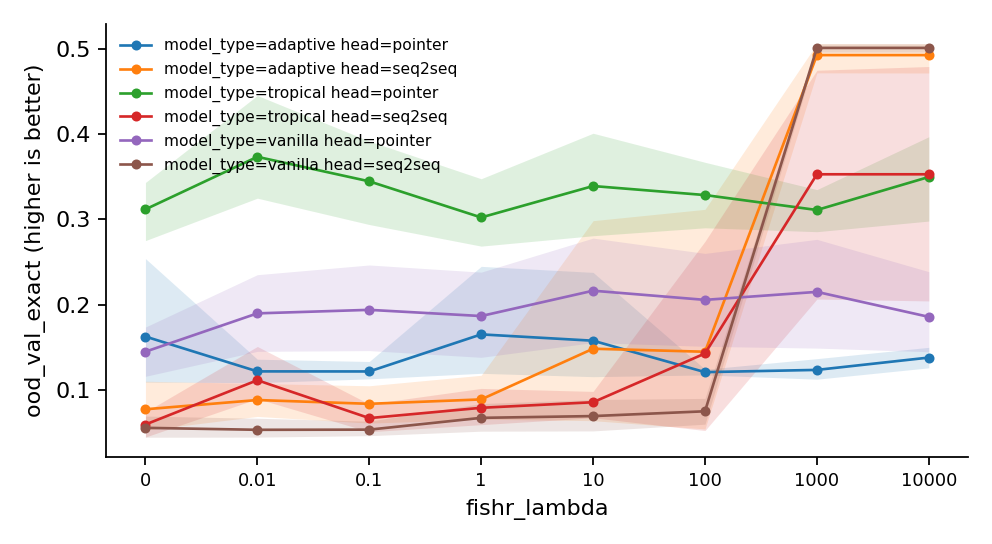
\includegraphics[width=\textwidth]{metric_ood_val_exact.png}
\caption{\texttt{ood\_val\_exact} against \texttt{fishr\_lambda}: the mean over seeds with a 95\% bootstrap CI, one line per combination of the other factors.}
\label{fig:ood_val_exact}
\end{figure}

{\small
\begin{longtable}{lllrlrrr}
\caption{\texttt{ood\_val\_exact} per cell: mean, 95\% bootstrap CI, SD, seeds, diverged runs.}\label{tab:summary-ood_val_exact}\\
\toprule
\texttt{model\_type} & \texttt{head} & \texttt{fishr\_lambda} & mean & 95\% CI & SD & $n$ & div.\\
\midrule
\endhead
adaptive & pointer & 0 & 0.1626 & [0.109, 0.254] & 0.102 & 5 & 0\\
adaptive & pointer & 0.01 & 0.1218 & [0.109, 0.136] & 0.0172 & 5 & 0\\
adaptive & pointer & 0.1 & 0.1217 & [0.113, 0.133] & 0.0134 & 5 & 0\\
adaptive & pointer & 1 & 0.1652 & [0.12, 0.245] & 0.0878 & 5 & 0\\
adaptive & pointer & 10 & 0.1578 & [0.116, 0.238] & 0.0895 & 5 & 0\\
adaptive & pointer & 100 & 0.1209 & [0.118, 0.124] & 0.00429 & 5 & 0\\
adaptive & pointer & 1000 & 0.1235 & [0.113, 0.137] & 0.0151 & 5 & 0\\
adaptive & pointer & 1e+04 & 0.138 & [0.126, 0.15] & 0.0159 & 5 & 0\\
adaptive & seq2seq & 0 & 0.07734 & [0.0528, 0.11] & 0.0369 & 5 & 0\\
adaptive & seq2seq & 0.01 & 0.08818 & [0.0689, 0.108] & 0.0242 & 5 & 0\\
adaptive & seq2seq & 0.1 & 0.08374 & [0.0611, 0.105] & 0.0291 & 5 & 0\\
adaptive & seq2seq & 1 & 0.0889 & [0.0657, 0.117] & 0.0341 & 5 & 0\\
adaptive & seq2seq & 10 & 0.1484 & [0.064, 0.299] & 0.167 & 5 & 0\\
adaptive & seq2seq & 100 & 0.1448 & [0.0543, 0.312] & 0.183 & 5 & 0\\
adaptive & seq2seq & 1000 & 0.4928 & [0.472, 0.506] & 0.0233 & 5 & 0\\
adaptive & seq2seq & 1e+04 & 0.4928 & [0.472, 0.506] & 0.0233 & 5 & 0\\
tropical & pointer & 0 & 0.3119 & [0.275, 0.343] & 0.0442 & 5 & 0\\
tropical & pointer & 0.01 & 0.3735 & [0.325, 0.445] & 0.0809 & 5 & 0\\
tropical & pointer & 0.1 & 0.3447 & [0.294, 0.392] & 0.0659 & 5 & 0\\
tropical & pointer & 1 & 0.3023 & [0.269, 0.348] & 0.0533 & 5 & 0\\
tropical & pointer & 10 & 0.3392 & [0.281, 0.401] & 0.0783 & 5 & 0\\
tropical & pointer & 100 & 0.3286 & [0.29, 0.367] & 0.0503 & 5 & 0\\
tropical & pointer & 1000 & 0.3111 & [0.286, 0.335] & 0.0324 & 5 & 0\\
tropical & pointer & 1e+04 & 0.3498 & [0.298, 0.397] & 0.0626 & 5 & 0\\
tropical & seq2seq & 0 & 0.05946 & [0.0448, 0.0742] & 0.0199 & 5 & 0\\
tropical & seq2seq & 0.01 & 0.1114 & [0.0897, 0.151] & 0.0441 & 5 & 0\\
tropical & seq2seq & 0.1 & 0.06698 & [0.051, 0.0835] & 0.0217 & 5 & 0\\
tropical & seq2seq & 1 & 0.07906 & [0.0593, 0.102] & 0.0288 & 5 & 0\\
tropical & seq2seq & 10 & 0.0856 & [0.0674, 0.0983] & 0.02 & 5 & 0\\
tropical & seq2seq & 100 & 0.1428 & [0.0524, 0.274] & 0.146 & 5 & 0\\
tropical & seq2seq & 1000 & 0.353 & [0.207, 0.475] & 0.177 & 5 & 0\\
tropical & seq2seq & 1e+04 & 0.353 & [0.204, 0.479] & 0.177 & 5 & 0\\
vanilla & pointer & 0 & 0.1449 & [0.116, 0.174] & 0.0375 & 5 & 0\\
vanilla & pointer & 0.01 & 0.1898 & [0.145, 0.235] & 0.0615 & 5 & 0\\
vanilla & pointer & 0.1 & 0.194 & [0.146, 0.247] & 0.0659 & 5 & 0\\
vanilla & pointer & 1 & 0.1867 & [0.138, 0.238] & 0.0667 & 5 & 0\\
vanilla & pointer & 10 & 0.2164 & [0.156, 0.278] & 0.0781 & 5 & 0\\
vanilla & pointer & 100 & 0.2057 & [0.151, 0.26] & 0.07 & 5 & 0\\
vanilla & pointer & 1000 & 0.215 & [0.149, 0.277] & 0.0787 & 5 & 0\\
vanilla & pointer & 1e+04 & 0.1857 & [0.145, 0.239] & 0.0602 & 5 & 0\\
vanilla & seq2seq & 0 & 0.05556 & [0.0445, 0.0694] & 0.0161 & 5 & 0\\
vanilla & seq2seq & 0.01 & 0.05326 & [0.0447, 0.0668] & 0.0145 & 5 & 0\\
vanilla & seq2seq & 0.1 & 0.05344 & [0.0464, 0.0633] & 0.0113 & 5 & 0\\
vanilla & seq2seq & 1 & 0.06728 & [0.0516, 0.084] & 0.0207 & 5 & 0\\
vanilla & seq2seq & 10 & 0.06936 & [0.0519, 0.0888] & 0.0234 & 5 & 0\\
vanilla & seq2seq & 100 & 0.07498 & [0.0599, 0.0901] & 0.0193 & 5 & 0\\
vanilla & seq2seq & 1000 & 0.5012 & [0.496, 0.506] & 0.00623 & 5 & 0\\
vanilla & seq2seq & 1e+04 & 0.5012 & [0.496, 0.506] & 0.00623 & 5 & 0\\
\bottomrule
\end{longtable}
}

{\small
\begin{longtable}{lllrrrl}
\caption{\texttt{ood\_val\_exact}: each level of \texttt{fishr\_lambda} against its control (0), within each combination of the other factors. parametric: Dunnett vs control.}\label{tab:control-ood_val_exact}\\
\toprule
\texttt{model\_type} & \texttt{head} & \texttt{fishr\_lambda} & difference & 95\% CI & $p$ & \\
\midrule
\endhead
adaptive & pointer & 0.01 & -0.04086 & [-0.142, 0.0607] & 0.7875 & \\
adaptive & pointer & 0.1 & -0.04094 & [-0.142, 0.0606] & 0.7863 & \\
adaptive & pointer & 1 & 0.00254 & [-0.099, 0.104] & 1.0000 & \\
adaptive & pointer & 10 & -0.00488 & [-0.106, 0.0966] & 1.0000 & \\
adaptive & pointer & 100 & -0.04174 & [-0.143, 0.0598] & 0.7720 & \\
adaptive & pointer & 1000 & -0.03912 & [-0.141, 0.0624] & 0.8171 & \\
adaptive & pointer & 1e+04 & -0.02466 & [-0.126, 0.0769] & 0.9761 & \\
adaptive & seq2seq & 0.01 & 0.01084 & [-0.148, 0.17] & 1.0000 & \\
adaptive & seq2seq & 0.1 & 0.0064 & [-0.153, 0.166] & 1.0000 & \\
adaptive & seq2seq & 1 & 0.01156 & [-0.148, 0.171] & 1.0000 & \\
adaptive & seq2seq & 10 & 0.07102 & [-0.0881, 0.23] & 0.7061 & \\
adaptive & seq2seq & 100 & 0.06748 & [-0.0917, 0.227] & 0.7483 & \\
adaptive & seq2seq & 1000 & 0.4154 & [0.256, 0.575] & $<10^{-4}$ & *\\
adaptive & seq2seq & 1e+04 & 0.4154 & [0.256, 0.575] & $<10^{-4}$ & *\\
tropical & pointer & 0.01 & 0.0616 & [-0.0441, 0.167] & 0.4461 & \\
tropical & pointer & 0.1 & 0.03284 & [-0.0729, 0.139] & 0.9223 & \\
tropical & pointer & 1 & -0.00952 & [-0.115, 0.0962] & 0.9999 & \\
tropical & pointer & 10 & 0.02734 & [-0.0784, 0.133] & 0.9672 & \\
tropical & pointer & 100 & 0.01676 & [-0.089, 0.123] & 0.9979 & \\
tropical & pointer & 1000 & $-7.800\times10^{-4}$ & [-0.107, 0.105] & 1.0000 & \\
tropical & pointer & 1e+04 & 0.03796 & [-0.0678, 0.144] & 0.8592 & \\
tropical & seq2seq & 0.01 & 0.05196 & [-0.131, 0.235] & 0.9481 & \\
tropical & seq2seq & 0.1 & 0.00752 & [-0.175, 0.19] & 1.0000 & \\
tropical & seq2seq & 1 & 0.0196 & [-0.163, 0.203] & 0.9998 & \\
tropical & seq2seq & 10 & 0.02614 & [-0.157, 0.209] & 0.9989 & \\
tropical & seq2seq & 100 & 0.08336 & [-0.0995, 0.266] & 0.6878 & \\
tropical & seq2seq & 1000 & 0.2935 & [0.111, 0.476] & 0.0006 & *\\
tropical & seq2seq & 1e+04 & 0.2935 & [0.111, 0.476] & 0.0007 & *\\
vanilla & pointer & 0.01 & 0.04494 & [-0.0703, 0.16] & 0.8090 & \\
vanilla & pointer & 0.1 & 0.04906 & [-0.0661, 0.164] & 0.7451 & \\
vanilla & pointer & 1 & 0.0418 & [-0.0734, 0.157] & 0.8533 & \\
vanilla & pointer & 10 & 0.07152 & [-0.0437, 0.187] & 0.3813 & \\
vanilla & pointer & 100 & 0.06076 & [-0.0544, 0.176] & 0.5479 & \\
vanilla & pointer & 1000 & 0.07014 & [-0.0451, 0.185] & 0.4009 & \\
vanilla & pointer & 1e+04 & 0.04084 & [-0.0744, 0.156] & 0.8658 & \\
vanilla & seq2seq & 0.01 & -0.0023 & [-0.0301, 0.0255] & 1.0000 & \\
vanilla & seq2seq & 0.1 & -0.00212 & [-0.0299, 0.0257] & 1.0000 & \\
vanilla & seq2seq & 1 & 0.01172 & [-0.0161, 0.0395] & 0.7523 & \\
vanilla & seq2seq & 10 & 0.0138 & [-0.014, 0.0416] & 0.6074 & \\
vanilla & seq2seq & 100 & 0.01942 & [-0.00836, 0.0472] & 0.2680 & \\
vanilla & seq2seq & 1000 & 0.4457 & [0.418, 0.473] & $<10^{-4}$ & *\\
vanilla & seq2seq & 1e+04 & 0.4457 & [0.418, 0.473] & $<10^{-4}$ & *\\
\bottomrule
\end{longtable}
}

{\small
\begin{longtable}{llrrrrr}
\caption{\texttt{ood\_val\_exact} against log10 \texttt{fishr\_lambda}: parametric: OLS slope t-test, seed-bootstrap CI, with the Jonckheere--Terpstra ordered-trend $\tau$ and $p$.}\label{tab:trend-ood_val_exact}\\
\toprule
\texttt{model\_type} & \texttt{head} & estimate & 95\% CI & $p$ & JT $\tau$ & JT $p$\\
\midrule
\endhead
adaptive & pointer & $2.843\times10^{-4}$ & [-0.0031, 0.00386] & 0.9451 & 0.158 & 0.2388\\
adaptive & seq2seq & 0.07456 & [0.07, 0.079] & $<10^{-4}$ & 0.419 & 0.0012\\
tropical & pointer & -0.003996 & [-0.0132, 0.00524] & 0.4472 & -0.0705 & 0.5921\\
tropical & seq2seq & 0.04859 & [0.0221, 0.069] & $<10^{-4}$ & 0.322 & 0.0162\\
vanilla & pointer & 0.001744 & [$-9.83\times10^{-4}$, 0.00543] & 0.7520 & -0.00952 & 0.9536\\
vanilla & seq2seq & 0.08025 & [0.0779, 0.0819] & $<10^{-4}$ & 0.68 & 0.0002\\
\bottomrule
\end{longtable}
}

{\small
\begin{longtable}{lrrrl}
\caption{\texttt{ood\_val\_exact}: paired contrasts by seed, Holm-corrected across the cells. parametric: paired t-test by seed, Holm.}\label{tab:paired-ood_val_exact}\\
\toprule
contrast (within) & difference & 95\% CI & $p$ & \\
\midrule
\endhead
\stackcell{model\_type: tropical - vanilla\\\footnotesize head=pointer fishr\_lambda=0 } & 0.167 & [0.0867, 0.247] & 0.0581 & \\
\stackcell{model\_type: tropical - vanilla\\\footnotesize head=pointer fishr\_lambda=0.01 } & 0.1836 & [0.115, 0.252] & 0.0284 & *\\
\stackcell{model\_type: tropical - vanilla\\\footnotesize head=pointer fishr\_lambda=0.1 } & 0.1507 & [0.0427, 0.259] & 0.1973 & \\
\stackcell{model\_type: tropical - vanilla\\\footnotesize head=pointer fishr\_lambda=1 } & 0.1156 & [0.0693, 0.162] & 0.0341 & *\\
\stackcell{model\_type: tropical - vanilla\\\footnotesize head=pointer fishr\_lambda=10 } & 0.1228 & [0.0433, 0.202] & 0.1532 & \\
\stackcell{model\_type: tropical - vanilla\\\footnotesize head=pointer fishr\_lambda=100 } & 0.123 & [0.0303, 0.216] & 0.2116 & \\
\stackcell{model\_type: tropical - vanilla\\\footnotesize head=pointer fishr\_lambda=1000 } & 0.09604 & [-0.0254, 0.217] & 0.7448 & \\
\stackcell{model\_type: tropical - vanilla\\\footnotesize head=pointer fishr\_lambda=1e+04 } & 0.1641 & [0.0871, 0.241] & 0.0572 & \\
\stackcell{model\_type: tropical - vanilla\\\footnotesize head=seq2seq fishr\_lambda=0 } & 0.0039 & [-0.0192, 0.027] & 1.0000 & \\
\stackcell{model\_type: tropical - vanilla\\\footnotesize head=seq2seq fishr\_lambda=0.01 } & 0.05816 & [-0.00486, 0.121] & 0.5624 & \\
\stackcell{model\_type: tropical - vanilla\\\footnotesize head=seq2seq fishr\_lambda=0.1 } & 0.01354 & [-0.0198, 0.0468] & 1.0000 & \\
\stackcell{model\_type: tropical - vanilla\\\footnotesize head=seq2seq fishr\_lambda=1 } & 0.01178 & [-0.0329, 0.0565] & 1.0000 & \\
\stackcell{model\_type: tropical - vanilla\\\footnotesize head=seq2seq fishr\_lambda=10 } & 0.01624 & [-0.0126, 0.0451] & 0.9707 & \\
\stackcell{model\_type: tropical - vanilla\\\footnotesize head=seq2seq fishr\_lambda=100 } & 0.06784 & [-0.12, 0.256] & 1.0000 & \\
\stackcell{model\_type: tropical - vanilla\\\footnotesize head=seq2seq fishr\_lambda=1000 } & -0.1482 & [-0.371, 0.0747] & 0.9707 & \\
\stackcell{model\_type: tropical - vanilla\\\footnotesize head=seq2seq fishr\_lambda=1e+04 } & -0.1482 & [-0.371, 0.0747] & 0.9707 & \\
\stackcell{model\_type: adaptive - vanilla\\\footnotesize head=pointer fishr\_lambda=0 } & 0.01774 & [-0.0775, 0.113] & 1.0000 & \\
\stackcell{model\_type: adaptive - vanilla\\\footnotesize head=pointer fishr\_lambda=0.01 } & -0.06806 & [-0.125, -0.0115] & 0.4318 & \\
\stackcell{model\_type: adaptive - vanilla\\\footnotesize head=pointer fishr\_lambda=0.1 } & -0.07226 & [-0.139, -0.00576] & 0.5443 & \\
\stackcell{model\_type: adaptive - vanilla\\\footnotesize head=pointer fishr\_lambda=1 } & -0.02152 & [-0.0863, 0.0433] & 1.0000 & \\
\stackcell{model\_type: adaptive - vanilla\\\footnotesize head=pointer fishr\_lambda=10 } & -0.05866 & [-0.172, 0.0546] & 1.0000 & \\
\stackcell{model\_type: adaptive - vanilla\\\footnotesize head=pointer fishr\_lambda=100 } & -0.08476 & [-0.172, 0.00236] & 0.5942 & \\
\stackcell{model\_type: adaptive - vanilla\\\footnotesize head=pointer fishr\_lambda=1000 } & -0.09152 & [-0.176, -0.00663] & 0.5443 & \\
\stackcell{model\_type: adaptive - vanilla\\\footnotesize head=pointer fishr\_lambda=1e+04 } & -0.04776 & [-0.116, 0.0208] & 1.0000 & \\
\stackcell{model\_type: adaptive - vanilla\\\footnotesize head=seq2seq fishr\_lambda=0 } & 0.02178 & [-0.0122, 0.0558] & 1.0000 & \\
\stackcell{model\_type: adaptive - vanilla\\\footnotesize head=seq2seq fishr\_lambda=0.01 } & 0.03492 & [0.0104, 0.0595] & 0.2686 & \\
\stackcell{model\_type: adaptive - vanilla\\\footnotesize head=seq2seq fishr\_lambda=0.1 } & 0.0303 & [0.00251, 0.0581] & 0.5443 & \\
\stackcell{model\_type: adaptive - vanilla\\\footnotesize head=seq2seq fishr\_lambda=1 } & 0.02162 & [-0.00791, 0.0511] & 1.0000 & \\
\stackcell{model\_type: adaptive - vanilla\\\footnotesize head=seq2seq fishr\_lambda=10 } & 0.079 & [-0.116, 0.274] & 1.0000 & \\
\stackcell{model\_type: adaptive - vanilla\\\footnotesize head=seq2seq fishr\_lambda=100 } & 0.06984 & [-0.146, 0.286] & 1.0000 & \\
\stackcell{model\_type: adaptive - vanilla\\\footnotesize head=seq2seq fishr\_lambda=1000 } & -0.00844 & [-0.0319, 0.015] & 1.0000 & \\
\stackcell{model\_type: adaptive - vanilla\\\footnotesize head=seq2seq fishr\_lambda=1e+04 } & -0.00844 & [-0.0319, 0.015] & 1.0000 & \\
\stackcell{head: pointer - seq2seq\\\footnotesize model\_type=adaptive fishr\_lambda=0 } & 0.0853 & [-0.0397, 0.21] & 0.7860 & \\
\stackcell{head: pointer - seq2seq\\\footnotesize model\_type=adaptive fishr\_lambda=0.01 } & 0.0336 & [-0.00218, 0.0694] & 0.4173 & \\
\stackcell{head: pointer - seq2seq\\\footnotesize model\_type=adaptive fishr\_lambda=0.1 } & 0.03796 & [$6.05\times10^{-4}$, 0.0753] & 0.3821 & \\
\stackcell{head: pointer - seq2seq\\\footnotesize model\_type=adaptive fishr\_lambda=1 } & 0.07628 & [-0.0438, 0.196] & 0.7860 & \\
\stackcell{head: pointer - seq2seq\\\footnotesize model\_type=adaptive fishr\_lambda=10 } & 0.0094 & [-0.247, 0.266] & 1.0000 & \\
\stackcell{head: pointer - seq2seq\\\footnotesize model\_type=adaptive fishr\_lambda=100 } & -0.02392 & [-0.254, 0.206] & 1.0000 & \\
\stackcell{head: pointer - seq2seq\\\footnotesize model\_type=adaptive fishr\_lambda=1000 } & -0.3693 & [-0.402, -0.336] & 0.0002 & *\\
\stackcell{head: pointer - seq2seq\\\footnotesize model\_type=adaptive fishr\_lambda=1e+04 } & -0.3548 & [-0.399, -0.311] & 0.0005 & *\\
\stackcell{head: pointer - seq2seq\\\footnotesize model\_type=tropical fishr\_lambda=0 } & 0.2524 & [0.174, 0.331] & 0.0177 & *\\
\stackcell{head: pointer - seq2seq\\\footnotesize model\_type=tropical fishr\_lambda=0.01 } & 0.262 & [0.211, 0.313] & 0.0030 & *\\
\stackcell{head: pointer - seq2seq\\\footnotesize model\_type=tropical fishr\_lambda=0.1 } & 0.2777 & [0.18, 0.376] & 0.0240 & *\\
\stackcell{head: pointer - seq2seq\\\footnotesize model\_type=tropical fishr\_lambda=1 } & 0.2233 & [0.151, 0.295] & 0.0192 & *\\
\stackcell{head: pointer - seq2seq\\\footnotesize model\_type=tropical fishr\_lambda=10 } & 0.2536 & [0.164, 0.344] & 0.0240 & *\\
\stackcell{head: pointer - seq2seq\\\footnotesize model\_type=tropical fishr\_lambda=100 } & 0.1858 & [0.0316, 0.34] & 0.2581 & \\
\stackcell{head: pointer - seq2seq\\\footnotesize model\_type=tropical fishr\_lambda=1000 } & -0.0419 & [-0.288, 0.204] & 1.0000 & \\
\stackcell{head: pointer - seq2seq\\\footnotesize model\_type=tropical fishr\_lambda=1e+04 } & -0.00316 & [-0.244, 0.238] & 1.0000 & \\
\stackcell{head: pointer - seq2seq\\\footnotesize model\_type=vanilla fishr\_lambda=0 } & 0.08934 & [0.0418, 0.137] & 0.0969 & \\
\stackcell{head: pointer - seq2seq\\\footnotesize model\_type=vanilla fishr\_lambda=0.01 } & 0.1366 & [0.0537, 0.22] & 0.1331 & \\
\stackcell{head: pointer - seq2seq\\\footnotesize model\_type=vanilla fishr\_lambda=0.1 } & 0.1405 & [0.054, 0.227] & 0.1331 & \\
\stackcell{head: pointer - seq2seq\\\footnotesize model\_type=vanilla fishr\_lambda=1 } & 0.1194 & [0.0258, 0.213] & 0.2396 & \\
\stackcell{head: pointer - seq2seq\\\footnotesize model\_type=vanilla fishr\_lambda=10 } & 0.1471 & [0.0597, 0.234] & 0.1326 & \\
\stackcell{head: pointer - seq2seq\\\footnotesize model\_type=vanilla fishr\_lambda=100 } & 0.1307 & [0.0484, 0.213] & 0.1331 & \\
\stackcell{head: pointer - seq2seq\\\footnotesize model\_type=vanilla fishr\_lambda=1000 } & -0.2862 & [-0.38, -0.192] & 0.0195 & *\\
\stackcell{head: pointer - seq2seq\\\footnotesize model\_type=vanilla fishr\_lambda=1e+04 } & -0.3155 & [-0.392, -0.239] & 0.0071 & *\\
\bottomrule
\end{longtable}
}

\subsection{\texttt{ood\_noise\_f1}}
\begin{figure}[tbp]
\centering
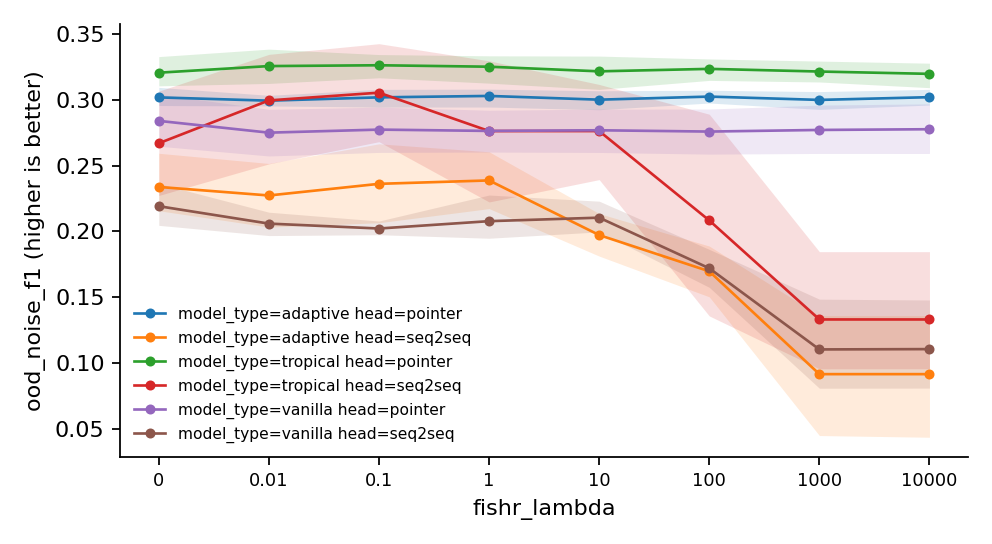
\includegraphics[width=\textwidth]{metric_ood_noise_f1.png}
\caption{\texttt{ood\_noise\_f1} against \texttt{fishr\_lambda}: the mean over seeds with a 95\% bootstrap CI, one line per combination of the other factors.}
\label{fig:ood_noise_f1}
\end{figure}

{\small
\begin{longtable}{lllrlrrr}
\caption{\texttt{ood\_noise\_f1} per cell: mean, 95\% bootstrap CI, SD, seeds, diverged runs.}\label{tab:summary-ood_noise_f1}\\
\toprule
\texttt{model\_type} & \texttt{head} & \texttt{fishr\_lambda} & mean & 95\% CI & SD & $n$ & div.\\
\midrule
\endhead
adaptive & pointer & 0 & 0.3018 & [0.296, 0.309] & 0.00889 & 5 & 0\\
adaptive & pointer & 0.01 & 0.2993 & [0.295, 0.303] & 0.00521 & 5 & 0\\
adaptive & pointer & 0.1 & 0.3018 & [0.294, 0.308] & 0.00852 & 5 & 0\\
adaptive & pointer & 1 & 0.3029 & [0.294, 0.308] & 0.00935 & 5 & 0\\
adaptive & pointer & 10 & 0.3001 & [0.292, 0.307] & 0.00995 & 5 & 0\\
adaptive & pointer & 100 & 0.3024 & [0.298, 0.307] & 0.00642 & 5 & 0\\
adaptive & pointer & 1000 & 0.2999 & [0.293, 0.306] & 0.00854 & 5 & 0\\
adaptive & pointer & 1e+04 & 0.3019 & [0.296, 0.308] & 0.00756 & 5 & 0\\
adaptive & seq2seq & 0 & 0.2338 & [0.216, 0.259] & 0.0289 & 5 & 0\\
adaptive & seq2seq & 0.01 & 0.2273 & [0.203, 0.252] & 0.0317 & 5 & 0\\
adaptive & seq2seq & 0.1 & 0.2361 & [0.207, 0.267] & 0.0399 & 5 & 0\\
adaptive & seq2seq & 1 & 0.2387 & [0.217, 0.26] & 0.028 & 5 & 0\\
adaptive & seq2seq & 10 & 0.1972 & [0.181, 0.214] & 0.0194 & 5 & 0\\
adaptive & seq2seq & 100 & 0.1697 & [0.15, 0.189] & 0.0246 & 5 & 0\\
adaptive & seq2seq & 1000 & 0.09155 & [0.0449, 0.136] & 0.0613 & 5 & 0\\
adaptive & seq2seq & 1e+04 & 0.09155 & [0.0436, 0.136] & 0.0613 & 5 & 0\\
tropical & pointer & 0 & 0.3206 & [0.311, 0.333] & 0.0136 & 5 & 0\\
tropical & pointer & 0.01 & 0.3256 & [0.312, 0.338] & 0.0157 & 5 & 0\\
tropical & pointer & 0.1 & 0.3262 & [0.317, 0.334] & 0.0114 & 5 & 0\\
tropical & pointer & 1 & 0.3251 & [0.313, 0.333] & 0.0139 & 5 & 0\\
tropical & pointer & 10 & 0.3216 & [0.308, 0.333] & 0.0158 & 5 & 0\\
tropical & pointer & 100 & 0.3235 & [0.315, 0.331] & 0.0101 & 5 & 0\\
tropical & pointer & 1000 & 0.3214 & [0.313, 0.329] & 0.0106 & 5 & 0\\
tropical & pointer & 1e+04 & 0.3197 & [0.309, 0.328] & 0.0122 & 5 & 0\\
tropical & seq2seq & 0 & 0.2669 & [0.227, 0.307] & 0.0516 & 5 & 0\\
tropical & seq2seq & 0.01 & 0.2995 & [0.251, 0.334] & 0.0562 & 5 & 0\\
tropical & seq2seq & 0.1 & 0.3054 & [0.268, 0.343] & 0.0482 & 5 & 0\\
tropical & seq2seq & 1 & 0.2762 & [0.222, 0.33] & 0.07 & 5 & 0\\
tropical & seq2seq & 10 & 0.2762 & [0.239, 0.312] & 0.0482 & 5 & 0\\
tropical & seq2seq & 100 & 0.2083 & [0.136, 0.289] & 0.0952 & 5 & 0\\
tropical & seq2seq & 1000 & 0.1331 & [0.0956, 0.185] & 0.0598 & 5 & 0\\
tropical & seq2seq & 1e+04 & 0.1331 & [0.0957, 0.185] & 0.0598 & 5 & 0\\
vanilla & pointer & 0 & 0.2839 & [0.265, 0.304] & 0.0248 & 5 & 0\\
vanilla & pointer & 0.01 & 0.275 & [0.257, 0.293] & 0.0231 & 5 & 0\\
vanilla & pointer & 0.1 & 0.2773 & [0.26, 0.294] & 0.0231 & 5 & 0\\
vanilla & pointer & 1 & 0.2763 & [0.26, 0.292] & 0.0218 & 5 & 0\\
vanilla & pointer & 10 & 0.2768 & [0.26, 0.293] & 0.0217 & 5 & 0\\
vanilla & pointer & 100 & 0.2758 & [0.259, 0.293] & 0.0235 & 5 & 0\\
vanilla & pointer & 1000 & 0.2771 & [0.259, 0.296] & 0.0241 & 5 & 0\\
vanilla & pointer & 1e+04 & 0.2776 & [0.259, 0.297] & 0.0248 & 5 & 0\\
vanilla & seq2seq & 0 & 0.2191 & [0.205, 0.236] & 0.0214 & 5 & 0\\
vanilla & seq2seq & 0.01 & 0.2059 & [0.197, 0.215] & 0.0118 & 5 & 0\\
vanilla & seq2seq & 0.1 & 0.2022 & [0.197, 0.208] & 0.00666 & 5 & 0\\
vanilla & seq2seq & 1 & 0.2078 & [0.195, 0.228] & 0.0218 & 5 & 0\\
vanilla & seq2seq & 10 & 0.2104 & [0.2, 0.223] & 0.0149 & 5 & 0\\
vanilla & seq2seq & 100 & 0.172 & [0.157, 0.186] & 0.0185 & 5 & 0\\
vanilla & seq2seq & 1000 & 0.1103 & [0.0808, 0.149] & 0.044 & 5 & 0\\
vanilla & seq2seq & 1e+04 & 0.1106 & [0.0809, 0.148] & 0.0437 & 5 & 0\\
\bottomrule
\end{longtable}
}

{\small
\begin{longtable}{lllrrrl}
\caption{\texttt{ood\_noise\_f1}: each level of \texttt{fishr\_lambda} against its control (0), within each combination of the other factors. parametric: Dunnett vs control.}\label{tab:control-ood_noise_f1}\\
\toprule
\texttt{model\_type} & \texttt{head} & \texttt{fishr\_lambda} & difference & 95\% CI & $p$ & \\
\midrule
\endhead
adaptive & pointer & 0.01 & -0.002487 & [-0.0168, 0.0118] & 0.9964 & \\
adaptive & pointer & 0.1 & $2.962\times10^{-5}$ & [-0.0143, 0.0143] & 1.0000 & \\
adaptive & pointer & 1 & 0.001109 & [-0.0132, 0.0154] & 1.0000 & \\
adaptive & pointer & 10 & -0.001728 & [-0.016, 0.0126] & 0.9996 & \\
adaptive & pointer & 100 & $6.115\times10^{-4}$ & [-0.0137, 0.0149] & 1.0000 & \\
adaptive & pointer & 1000 & -0.001907 & [-0.0162, 0.0124] & 0.9993 & \\
adaptive & pointer & 1e+04 & $1.639\times10^{-4}$ & [-0.0141, 0.0145] & 1.0000 & \\
adaptive & seq2seq & 0.01 & -0.006479 & [-0.0761, 0.0631] & 0.9999 & \\
adaptive & seq2seq & 0.1 & 0.002361 & [-0.0673, 0.072] & 1.0000 & \\
adaptive & seq2seq & 1 & 0.004944 & [-0.0647, 0.0746] & 1.0000 & \\
adaptive & seq2seq & 10 & -0.03655 & [-0.106, 0.0331] & 0.5526 & \\
adaptive & seq2seq & 100 & -0.06409 & [-0.134, 0.00553] & 0.0813 & \\
adaptive & seq2seq & 1000 & -0.1422 & [-0.212, -0.0726] & $<10^{-4}$ & *\\
adaptive & seq2seq & 1e+04 & -0.1422 & [-0.212, -0.0726] & $<10^{-4}$ & *\\
tropical & pointer & 0.01 & 0.005024 & [-0.0178, 0.0279] & 0.9860 & \\
tropical & pointer & 0.1 & 0.005645 & [-0.0172, 0.0285] & 0.9739 & \\
tropical & pointer & 1 & 0.004544 & [-0.0183, 0.0274] & 0.9920 & \\
tropical & pointer & 10 & 0.001028 & [-0.0218, 0.0239] & 1.0000 & \\
tropical & pointer & 100 & 0.002901 & [-0.0199, 0.0257] & 0.9995 & \\
tropical & pointer & 1000 & $8.828\times10^{-4}$ & [-0.022, 0.0237] & 1.0000 & \\
tropical & pointer & 1e+04 & $-8.864\times10^{-4}$ & [-0.0237, 0.022] & 1.0000 & \\
tropical & seq2seq & 0.01 & 0.03255 & [-0.0772, 0.142] & 0.9367 & \\
tropical & seq2seq & 0.1 & 0.03843 & [-0.0713, 0.148] & 0.8722 & \\
tropical & seq2seq & 1 & 0.009271 & [-0.1, 0.119] & 1.0000 & \\
tropical & seq2seq & 10 & 0.009266 & [-0.1, 0.119] & 1.0000 & \\
tropical & seq2seq & 100 & -0.05862 & [-0.168, 0.0511] & 0.5350 & \\
tropical & seq2seq & 1000 & -0.1339 & [-0.244, -0.0241] & 0.0115 & *\\
tropical & seq2seq & 1e+04 & -0.1339 & [-0.244, -0.0241] & 0.0116 & *\\
vanilla & pointer & 0.01 & -0.008953 & [-0.0498, 0.0319] & 0.9863 & \\
vanilla & pointer & 0.1 & -0.006635 & [-0.0475, 0.0343] & 0.9976 & \\
vanilla & pointer & 1 & -0.007635 & [-0.0485, 0.0333] & 0.9944 & \\
vanilla & pointer & 10 & -0.007142 & [-0.048, 0.0338] & 0.9963 & \\
vanilla & pointer & 100 & -0.008125 & [-0.049, 0.0328] & 0.9920 & \\
vanilla & pointer & 1000 & -0.006896 & [-0.0478, 0.034] & 0.9970 & \\
vanilla & pointer & 1e+04 & -0.006344 & [-0.0472, 0.0346] & 0.9982 & \\
vanilla & seq2seq & 0.01 & -0.01322 & [-0.0592, 0.0327] & 0.9449 & \\
vanilla & seq2seq & 0.1 & -0.01695 & [-0.0629, 0.029] & 0.8437 & \\
vanilla & seq2seq & 1 & -0.01137 & [-0.0573, 0.0346] & 0.9737 & \\
vanilla & seq2seq & 10 & -0.008713 & [-0.0547, 0.0372] & 0.9939 & \\
vanilla & seq2seq & 100 & -0.04716 & [-0.0931, -0.00122] & 0.0422 & *\\
vanilla & seq2seq & 1000 & -0.1088 & [-0.155, -0.0629] & $<10^{-4}$ & *\\
vanilla & seq2seq & 1e+04 & -0.1086 & [-0.155, -0.0626] & $<10^{-4}$ & *\\
\bottomrule
\end{longtable}
}

{\small
\begin{longtable}{llrrrrr}
\caption{\texttt{ood\_noise\_f1} against log10 \texttt{fishr\_lambda}: parametric: OLS slope t-test, seed-bootstrap CI, with the Jonckheere--Terpstra ordered-trend $\tau$ and $p$.}\label{tab:trend-ood_noise_f1}\\
\toprule
\texttt{model\_type} & \texttt{head} & estimate & 95\% CI & $p$ & JT $\tau$ & JT $p$\\
\midrule
\endhead
adaptive & pointer & $1.279\times10^{-4}$ & [$-2.69\times10^{-4}$, $5.79\times10^{-4}$] & 0.8426 & 0.0552 & 0.6965\\
adaptive & seq2seq & -0.02733 & [-0.0397, -0.015] & $<10^{-4}$ & -0.716 & 0.0002\\
tropical & pointer & -0.001032 & [-0.00177, $-2.35\times10^{-4}$] & 0.3169 & -0.135 & 0.3177\\
tropical & seq2seq & -0.03256 & [-0.0405, -0.0245] & $<10^{-4}$ & -0.547 & 0.0002\\
vanilla & pointer & $2.433\times10^{-4}$ & [$-1.14\times10^{-4}$, $6.83\times10^{-4}$] & 0.8937 & -0.0019 & 1.0000\\
vanilla & seq2seq & -0.01805 & [-0.0244, -0.0105] & $<10^{-4}$ & -0.577 & 0.0002\\
\bottomrule
\end{longtable}
}

{\small
\begin{longtable}{lrrrl}
\caption{\texttt{ood\_noise\_f1}: paired contrasts by seed, Holm-corrected across the cells. parametric: paired t-test by seed, Holm.}\label{tab:paired-ood_noise_f1}\\
\toprule
contrast (within) & difference & 95\% CI & $p$ & \\
\midrule
\endhead
\stackcell{model\_type: tropical - vanilla\\\footnotesize head=pointer fishr\_lambda=0 } & 0.0366 & [-0.00401, 0.0772] & 0.3995 & \\
\stackcell{model\_type: tropical - vanilla\\\footnotesize head=pointer fishr\_lambda=0.01 } & 0.05058 & [0.00765, 0.0935] & 0.3987 & \\
\stackcell{model\_type: tropical - vanilla\\\footnotesize head=pointer fishr\_lambda=0.1 } & 0.04888 & [0.00841, 0.0894] & 0.3987 & \\
\stackcell{model\_type: tropical - vanilla\\\footnotesize head=pointer fishr\_lambda=1 } & 0.04878 & [0.00794, 0.0896] & 0.3987 & \\
\stackcell{model\_type: tropical - vanilla\\\footnotesize head=pointer fishr\_lambda=10 } & 0.04477 & [0.00523, 0.0843] & 0.3987 & \\
\stackcell{model\_type: tropical - vanilla\\\footnotesize head=pointer fishr\_lambda=100 } & 0.04763 & [0.0095, 0.0858] & 0.3843 & \\
\stackcell{model\_type: tropical - vanilla\\\footnotesize head=pointer fishr\_lambda=1000 } & 0.04438 & [0.00605, 0.0827] & 0.3987 & \\
\stackcell{model\_type: tropical - vanilla\\\footnotesize head=pointer fishr\_lambda=1e+04 } & 0.04206 & [0.00156, 0.0826] & 0.3987 & \\
\stackcell{model\_type: tropical - vanilla\\\footnotesize head=seq2seq fishr\_lambda=0 } & 0.04781 & [-0.0214, 0.117] & 0.5096 & \\
\stackcell{model\_type: tropical - vanilla\\\footnotesize head=seq2seq fishr\_lambda=0.01 } & 0.09358 & [0.016, 0.171] & 0.3987 & \\
\stackcell{model\_type: tropical - vanilla\\\footnotesize head=seq2seq fishr\_lambda=0.1 } & 0.1032 & [0.036, 0.17] & 0.2078 & \\
\stackcell{model\_type: tropical - vanilla\\\footnotesize head=seq2seq fishr\_lambda=1 } & 0.06845 & [-0.0119, 0.149] & 0.3995 & \\
\stackcell{model\_type: tropical - vanilla\\\footnotesize head=seq2seq fishr\_lambda=10 } & 0.06579 & [-0.00118, 0.133] & 0.3987 & \\
\stackcell{model\_type: tropical - vanilla\\\footnotesize head=seq2seq fishr\_lambda=100 } & 0.03634 & [-0.0817, 0.154] & 1.0000 & \\
\stackcell{model\_type: tropical - vanilla\\\footnotesize head=seq2seq fishr\_lambda=1000 } & 0.02276 & [-0.0863, 0.132] & 1.0000 & \\
\stackcell{model\_type: tropical - vanilla\\\footnotesize head=seq2seq fishr\_lambda=1e+04 } & 0.02251 & [-0.0864, 0.131] & 1.0000 & \\
\stackcell{model\_type: adaptive - vanilla\\\footnotesize head=pointer fishr\_lambda=0 } & 0.01784 & [-0.0124, 0.0481] & 1.0000 & \\
\stackcell{model\_type: adaptive - vanilla\\\footnotesize head=pointer fishr\_lambda=0.01 } & 0.0243 & [$-1.06\times10^{-4}$, 0.0487] & 0.5062 & \\
\stackcell{model\_type: adaptive - vanilla\\\footnotesize head=pointer fishr\_lambda=0.1 } & 0.0245 & [0.00451, 0.0445] & 0.3811 & \\
\stackcell{model\_type: adaptive - vanilla\\\footnotesize head=pointer fishr\_lambda=1 } & 0.02658 & [0.00783, 0.0453] & 0.2555 & \\
\stackcell{model\_type: adaptive - vanilla\\\footnotesize head=pointer fishr\_lambda=10 } & 0.02325 & [0.00731, 0.0392] & 0.2478 & \\
\stackcell{model\_type: adaptive - vanilla\\\footnotesize head=pointer fishr\_lambda=100 } & 0.02657 & [0.00336, 0.0498] & 0.4364 & \\
\stackcell{model\_type: adaptive - vanilla\\\footnotesize head=pointer fishr\_lambda=1000 } & 0.02282 & [$9.24\times10^{-4}$, 0.0447] & 0.4884 & \\
\stackcell{model\_type: adaptive - vanilla\\\footnotesize head=pointer fishr\_lambda=1e+04 } & 0.02434 & [0.00252, 0.0462] & 0.4364 & \\
\stackcell{model\_type: adaptive - vanilla\\\footnotesize head=seq2seq fishr\_lambda=0 } & 0.01463 & [-0.0229, 0.0522] & 1.0000 & \\
\stackcell{model\_type: adaptive - vanilla\\\footnotesize head=seq2seq fishr\_lambda=0.01 } & 0.02137 & [-0.0082, 0.0509] & 0.9223 & \\
\stackcell{model\_type: adaptive - vanilla\\\footnotesize head=seq2seq fishr\_lambda=0.1 } & 0.03394 & [-0.0141, 0.082] & 0.9223 & \\
\stackcell{model\_type: adaptive - vanilla\\\footnotesize head=seq2seq fishr\_lambda=1 } & 0.03094 & [-0.00587, 0.0677] & 0.7194 & \\
\stackcell{model\_type: adaptive - vanilla\\\footnotesize head=seq2seq fishr\_lambda=10 } & -0.01321 & [-0.0485, 0.0221] & 1.0000 & \\
\stackcell{model\_type: adaptive - vanilla\\\footnotesize head=seq2seq fishr\_lambda=100 } & -0.002305 & [-0.0473, 0.0427] & 1.0000 & \\
\stackcell{model\_type: adaptive - vanilla\\\footnotesize head=seq2seq fishr\_lambda=1000 } & -0.01877 & [-0.104, 0.0664] & 1.0000 & \\
\stackcell{model\_type: adaptive - vanilla\\\footnotesize head=seq2seq fishr\_lambda=1e+04 } & -0.01902 & [-0.104, 0.0664] & 1.0000 & \\
\stackcell{head: pointer - seq2seq\\\footnotesize model\_type=adaptive fishr\_lambda=0 } & 0.06803 & [0.0274, 0.109] & 0.1060 & \\
\stackcell{head: pointer - seq2seq\\\footnotesize model\_type=adaptive fishr\_lambda=0.01 } & 0.07202 & [0.0321, 0.112] & 0.0975 & \\
\stackcell{head: pointer - seq2seq\\\footnotesize model\_type=adaptive fishr\_lambda=0.1 } & 0.06569 & [0.0105, 0.121] & 0.2081 & \\
\stackcell{head: pointer - seq2seq\\\footnotesize model\_type=adaptive fishr\_lambda=1 } & 0.06419 & [0.0215, 0.107] & 0.1259 & \\
\stackcell{head: pointer - seq2seq\\\footnotesize model\_type=adaptive fishr\_lambda=10 } & 0.1028 & [0.0684, 0.137] & 0.0266 & *\\
\stackcell{head: pointer - seq2seq\\\footnotesize model\_type=adaptive fishr\_lambda=100 } & 0.1327 & [0.0967, 0.169] & 0.0124 & *\\
\stackcell{head: pointer - seq2seq\\\footnotesize model\_type=adaptive fishr\_lambda=1000 } & 0.2083 & [0.134, 0.282] & 0.0303 & *\\
\stackcell{head: pointer - seq2seq\\\footnotesize model\_type=adaptive fishr\_lambda=1e+04 } & 0.2104 & [0.14, 0.281] & 0.0266 & *\\
\stackcell{head: pointer - seq2seq\\\footnotesize model\_type=tropical fishr\_lambda=0 } & 0.05361 & [$-9.40\times10^{-4}$, 0.108] & 0.2825 & \\
\stackcell{head: pointer - seq2seq\\\footnotesize model\_type=tropical fishr\_lambda=0.01 } & 0.02609 & [-0.0401, 0.0922] & 0.6700 & \\
\stackcell{head: pointer - seq2seq\\\footnotesize model\_type=tropical fishr\_lambda=0.1 } & 0.02083 & [-0.0345, 0.0762] & 0.6700 & \\
\stackcell{head: pointer - seq2seq\\\footnotesize model\_type=tropical fishr\_lambda=1 } & 0.04889 & [-0.0326, 0.13] & 0.5469 & \\
\stackcell{head: pointer - seq2seq\\\footnotesize model\_type=tropical fishr\_lambda=10 } & 0.04537 & [-0.0224, 0.113] & 0.5469 & \\
\stackcell{head: pointer - seq2seq\\\footnotesize model\_type=tropical fishr\_lambda=100 } & 0.1151 & [0.0024, 0.228] & 0.2825 & \\
\stackcell{head: pointer - seq2seq\\\footnotesize model\_type=tropical fishr\_lambda=1000 } & 0.1884 & [0.119, 0.258] & 0.0303 & *\\
\stackcell{head: pointer - seq2seq\\\footnotesize model\_type=tropical fishr\_lambda=1e+04 } & 0.1866 & [0.119, 0.255] & 0.0303 & *\\
\stackcell{head: pointer - seq2seq\\\footnotesize model\_type=vanilla fishr\_lambda=0 } & 0.06482 & [0.0148, 0.115] & 0.1819 & \\
\stackcell{head: pointer - seq2seq\\\footnotesize model\_type=vanilla fishr\_lambda=0.01 } & 0.06909 & [0.0312, 0.107] & 0.0975 & \\
\stackcell{head: pointer - seq2seq\\\footnotesize model\_type=vanilla fishr\_lambda=0.1 } & 0.07514 & [0.0482, 0.102] & 0.0303 & *\\
\stackcell{head: pointer - seq2seq\\\footnotesize model\_type=vanilla fishr\_lambda=1 } & 0.06855 & [0.0313, 0.106] & 0.0975 & \\
\stackcell{head: pointer - seq2seq\\\footnotesize model\_type=vanilla fishr\_lambda=10 } & 0.06639 & [0.0262, 0.107] & 0.1060 & \\
\stackcell{head: pointer - seq2seq\\\footnotesize model\_type=vanilla fishr\_lambda=100 } & 0.1039 & [0.0624, 0.145] & 0.0382 & *\\
\stackcell{head: pointer - seq2seq\\\footnotesize model\_type=vanilla fishr\_lambda=1000 } & 0.1667 & [0.0917, 0.242] & 0.0561 & \\
\stackcell{head: pointer - seq2seq\\\footnotesize model\_type=vanilla fishr\_lambda=1e+04 } & 0.167 & [0.0916, 0.243] & 0.0561 & \\
\bottomrule
\end{longtable}
}

\subsection{\texttt{ood\_noise\_exact}}
\begin{figure}[tbp]
\centering
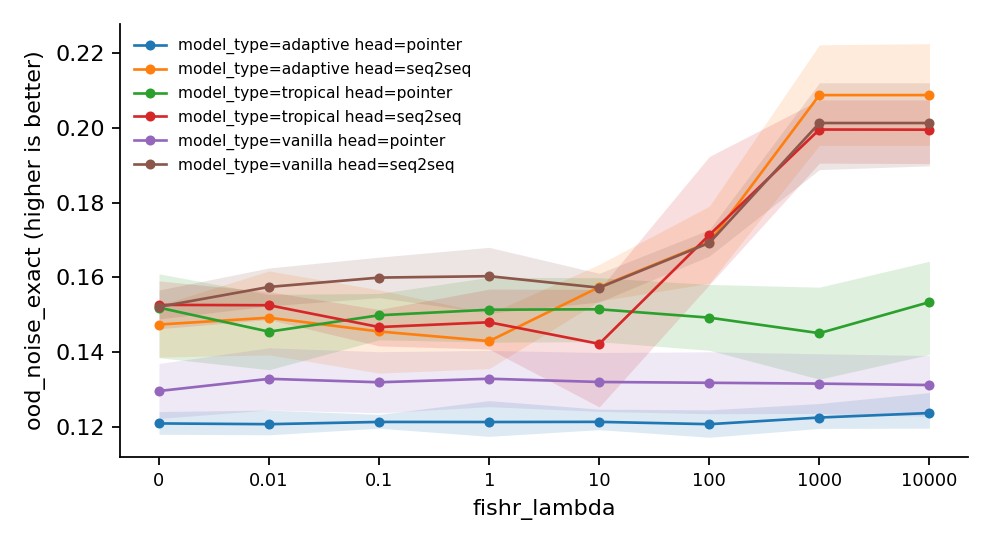
\includegraphics[width=\textwidth]{metric_ood_noise_exact.png}
\caption{\texttt{ood\_noise\_exact} against \texttt{fishr\_lambda}: the mean over seeds with a 95\% bootstrap CI, one line per combination of the other factors.}
\label{fig:ood_noise_exact}
\end{figure}

{\small
\begin{longtable}{lllrlrrr}
\caption{\texttt{ood\_noise\_exact} per cell: mean, 95\% bootstrap CI, SD, seeds, diverged runs.}\label{tab:summary-ood_noise_exact}\\
\toprule
\texttt{model\_type} & \texttt{head} & \texttt{fishr\_lambda} & mean & 95\% CI & SD & $n$ & div.\\
\midrule
\endhead
adaptive & pointer & 0 & 0.1209 & [0.118, 0.124] & 0.00404 & 5 & 0\\
adaptive & pointer & 0.01 & 0.1207 & [0.118, 0.124] & 0.00429 & 5 & 0\\
adaptive & pointer & 0.1 & 0.1213 & [0.12, 0.123] & 0.0025 & 5 & 0\\
adaptive & pointer & 1 & 0.1213 & [0.117, 0.127] & 0.0062 & 5 & 0\\
adaptive & pointer & 10 & 0.1213 & [0.119, 0.125] & 0.00376 & 5 & 0\\
adaptive & pointer & 100 & 0.1207 & [0.117, 0.125] & 0.00491 & 5 & 0\\
adaptive & pointer & 1000 & 0.1225 & [0.12, 0.126] & 0.00444 & 5 & 0\\
adaptive & pointer & 1e+04 & 0.1237 & [0.12, 0.129] & 0.00636 & 5 & 0\\
adaptive & seq2seq & 0 & 0.1474 & [0.139, 0.153] & 0.00974 & 5 & 0\\
adaptive & seq2seq & 0.01 & 0.1492 & [0.139, 0.162] & 0.015 & 5 & 0\\
adaptive & seq2seq & 0.1 & 0.1455 & [0.134, 0.157] & 0.0153 & 5 & 0\\
adaptive & seq2seq & 1 & 0.1429 & [0.136, 0.15] & 0.00954 & 5 & 0\\
adaptive & seq2seq & 10 & 0.1574 & [0.154, 0.163] & 0.00691 & 5 & 0\\
adaptive & seq2seq & 100 & 0.1694 & [0.158, 0.179] & 0.0131 & 5 & 0\\
adaptive & seq2seq & 1000 & 0.2088 & [0.195, 0.222] & 0.0179 & 5 & 0\\
adaptive & seq2seq & 1e+04 & 0.2088 & [0.195, 0.223] & 0.0179 & 5 & 0\\
tropical & pointer & 0 & 0.1519 & [0.139, 0.161] & 0.015 & 5 & 0\\
tropical & pointer & 0.01 & 0.1455 & [0.135, 0.155] & 0.0131 & 5 & 0\\
tropical & pointer & 0.1 & 0.1499 & [0.143, 0.156] & 0.00805 & 5 & 0\\
tropical & pointer & 1 & 0.1513 & [0.143, 0.16] & 0.0117 & 5 & 0\\
tropical & pointer & 10 & 0.1515 & [0.143, 0.16] & 0.0114 & 5 & 0\\
tropical & pointer & 100 & 0.1492 & [0.14, 0.158] & 0.0119 & 5 & 0\\
tropical & pointer & 1000 & 0.1451 & [0.133, 0.157] & 0.0157 & 5 & 0\\
tropical & pointer & 1e+04 & 0.1534 & [0.139, 0.164] & 0.0163 & 5 & 0\\
tropical & seq2seq & 0 & 0.1526 & [0.146, 0.159] & 0.00834 & 5 & 0\\
tropical & seq2seq & 0.01 & 0.1525 & [0.149, 0.156] & 0.005 & 5 & 0\\
tropical & seq2seq & 0.1 & 0.1467 & [0.142, 0.151] & 0.00628 & 5 & 0\\
tropical & seq2seq & 1 & 0.148 & [0.141, 0.157] & 0.0106 & 5 & 0\\
tropical & seq2seq & 10 & 0.1422 & [0.125, 0.157] & 0.0199 & 5 & 0\\
tropical & seq2seq & 100 & 0.1714 & [0.158, 0.192] & 0.0232 & 5 & 0\\
tropical & seq2seq & 1000 & 0.1996 & [0.191, 0.208] & 0.0107 & 5 & 0\\
tropical & seq2seq & 1e+04 & 0.1995 & [0.19, 0.208] & 0.0108 & 5 & 0\\
vanilla & pointer & 0 & 0.1296 & [0.122, 0.137] & 0.00952 & 5 & 0\\
vanilla & pointer & 0.01 & 0.1328 & [0.125, 0.141] & 0.0107 & 5 & 0\\
vanilla & pointer & 0.1 & 0.1319 & [0.124, 0.14] & 0.0105 & 5 & 0\\
vanilla & pointer & 1 & 0.1329 & [0.125, 0.14] & 0.00968 & 5 & 0\\
vanilla & pointer & 10 & 0.132 & [0.124, 0.14] & 0.0101 & 5 & 0\\
vanilla & pointer & 100 & 0.1318 & [0.124, 0.14] & 0.0104 & 5 & 0\\
vanilla & pointer & 1000 & 0.1316 & [0.124, 0.14] & 0.01 & 5 & 0\\
vanilla & pointer & 1e+04 & 0.1312 & [0.123, 0.139] & 0.0108 & 5 & 0\\
vanilla & seq2seq & 0 & 0.1521 & [0.149, 0.157] & 0.00519 & 5 & 0\\
vanilla & seq2seq & 0.01 & 0.1574 & [0.152, 0.163] & 0.00665 & 5 & 0\\
vanilla & seq2seq & 0.1 & 0.1599 & [0.155, 0.165] & 0.00707 & 5 & 0\\
vanilla & seq2seq & 1 & 0.1603 & [0.15, 0.168] & 0.0118 & 5 & 0\\
vanilla & seq2seq & 10 & 0.1572 & [0.153, 0.161] & 0.005 & 5 & 0\\
vanilla & seq2seq & 100 & 0.1692 & [0.166, 0.173] & 0.00463 & 5 & 0\\
vanilla & seq2seq & 1000 & 0.2013 & [0.189, 0.212] & 0.0141 & 5 & 0\\
vanilla & seq2seq & 1e+04 & 0.2013 & [0.19, 0.212] & 0.0141 & 5 & 0\\
\bottomrule
\end{longtable}
}

{\small
\begin{longtable}{lllrrrl}
\caption{\texttt{ood\_noise\_exact}: each level of \texttt{fishr\_lambda} against its control (0), within each combination of the other factors. parametric: Dunnett vs control.}\label{tab:control-ood_noise_exact}\\
\toprule
\texttt{model\_type} & \texttt{head} & \texttt{fishr\_lambda} & difference & 95\% CI & $p$ & \\
\midrule
\endhead
adaptive & pointer & 0.01 & $-2.000\times10^{-4}$ & [-0.00844, 0.00804] & 1.0000 & \\
adaptive & pointer & 0.1 & $4.000\times10^{-4}$ & [-0.00784, 0.00864] & 1.0000 & \\
adaptive & pointer & 1 & $3.800\times10^{-4}$ & [-0.00786, 0.00862] & 1.0000 & \\
adaptive & pointer & 10 & $4.200\times10^{-4}$ & [-0.00782, 0.00866] & 1.0000 & \\
adaptive & pointer & 100 & $-2.000\times10^{-4}$ & [-0.00844, 0.00804] & 1.0000 & \\
adaptive & pointer & 1000 & 0.00158 & [-0.00666, 0.00982] & 0.9935 & \\
adaptive & pointer & 1e+04 & 0.00278 & [-0.00546, 0.011] & 0.8895 & \\
adaptive & seq2seq & 0.01 & 0.00182 & [-0.0221, 0.0258] & 1.0000 & \\
adaptive & seq2seq & 0.1 & -0.00186 & [-0.0258, 0.0221] & 1.0000 & \\
adaptive & seq2seq & 1 & -0.00444 & [-0.0284, 0.0195] & 0.9947 & \\
adaptive & seq2seq & 10 & 0.01002 & [-0.0139, 0.034] & 0.7587 & \\
adaptive & seq2seq & 100 & 0.02206 & [-0.00189, 0.046] & 0.0810 & \\
adaptive & seq2seq & 1000 & 0.06142 & [0.0375, 0.0854] & $<10^{-4}$ & *\\
adaptive & seq2seq & 1e+04 & 0.06142 & [0.0375, 0.0854] & $<10^{-4}$ & *\\
tropical & pointer & 0.01 & -0.00644 & [-0.0294, 0.0165] & 0.9514 & \\
tropical & pointer & 0.1 & -0.00204 & [-0.025, 0.0209] & 1.0000 & \\
tropical & pointer & 1 & $-5.600\times10^{-4}$ & [-0.0235, 0.0224] & 1.0000 & \\
tropical & pointer & 10 & $-4.400\times10^{-4}$ & [-0.0234, 0.0225] & 1.0000 & \\
tropical & pointer & 100 & -0.00268 & [-0.0257, 0.0203] & 0.9997 & \\
tropical & pointer & 1000 & -0.00684 & [-0.0298, 0.0161] & 0.9358 & \\
tropical & pointer & 1e+04 & 0.00148 & [-0.0215, 0.0245] & 1.0000 & \\
tropical & seq2seq & 0.01 & $-1.000\times10^{-4}$ & [-0.0233, 0.0231] & 1.0000 & \\
tropical & seq2seq & 0.1 & -0.00594 & [-0.0292, 0.0173] & 0.9690 & \\
tropical & seq2seq & 1 & -0.00466 & [-0.0279, 0.0186] & 0.9916 & \\
tropical & seq2seq & 10 & -0.01044 & [-0.0337, 0.0128] & 0.7004 & \\
tropical & seq2seq & 100 & 0.01872 & [-0.00452, 0.042] & 0.1562 & \\
tropical & seq2seq & 1000 & 0.04694 & [0.0237, 0.0702] & $<10^{-4}$ & *\\
tropical & seq2seq & 1e+04 & 0.0469 & [0.0237, 0.0701] & $<10^{-4}$ & *\\
vanilla & pointer & 0.01 & 0.00326 & [-0.0146, 0.0211] & 0.9951 & \\
vanilla & pointer & 0.1 & 0.00234 & [-0.0155, 0.0202] & 0.9994 & \\
vanilla & pointer & 1 & 0.00328 & [-0.0146, 0.0211] & 0.9949 & \\
vanilla & pointer & 10 & 0.00242 & [-0.0154, 0.0203] & 0.9992 & \\
vanilla & pointer & 100 & 0.0022 & [-0.0156, 0.02] & 0.9996 & \\
vanilla & pointer & 1000 & 0.00198 & [-0.0159, 0.0198] & 0.9998 & \\
vanilla & pointer & 1e+04 & 0.0016 & [-0.0162, 0.0194] & 0.9999 & \\
vanilla & seq2seq & 0.01 & 0.00532 & [-0.0111, 0.0218] & 0.9070 & \\
vanilla & seq2seq & 0.1 & 0.00782 & [-0.00861, 0.0243] & 0.6485 & \\
vanilla & seq2seq & 1 & 0.0082 & [-0.00823, 0.0246] & 0.6030 & \\
vanilla & seq2seq & 10 & 0.00512 & [-0.0113, 0.0216] & 0.9211 & \\
vanilla & seq2seq & 100 & 0.01712 & [$6.90\times10^{-4}$, 0.0336] & 0.0382 & *\\
vanilla & seq2seq & 1000 & 0.0492 & [0.0328, 0.0656] & $<10^{-4}$ & *\\
vanilla & seq2seq & 1e+04 & 0.0492 & [0.0328, 0.0656] & $<10^{-4}$ & *\\
\bottomrule
\end{longtable}
}

{\small
\begin{longtable}{llrrrrr}
\caption{\texttt{ood\_noise\_exact} against log10 \texttt{fishr\_lambda}: parametric: OLS slope t-test, seed-bootstrap CI, with the Jonckheere--Terpstra ordered-trend $\tau$ and $p$.}\label{tab:trend-ood_noise_exact}\\
\toprule
\texttt{model\_type} & \texttt{head} & estimate & 95\% CI & $p$ & JT $\tau$ & JT $p$\\
\midrule
\endhead
adaptive & pointer & $3.829\times10^{-4}$ & [$4.36\times10^{-5}$, $7.22\times10^{-4}$] & 0.3187 & 0.149 & 0.2577\\
adaptive & seq2seq & 0.01185 & [0.0074, 0.0163] & $<10^{-4}$ & 0.705 & 0.0002\\
tropical & pointer & $4.300\times10^{-4}$ & [$-4.55\times10^{-4}$, 0.00109] & 0.6792 & 0.0724 & 0.6011\\
tropical & seq2seq & 0.009648 & [0.00732, 0.012] & $<10^{-4}$ & 0.539 & 0.0004\\
vanilla & pointer & $-2.421\times10^{-4}$ & [$-3.68\times10^{-4}$, $-7.50\times10^{-5}$] & 0.7650 & -0.114 & 0.4017\\
vanilla & seq2seq & 0.007976 & [0.00568, 0.0102] & $<10^{-4}$ & 0.634 & 0.0002\\
\bottomrule
\end{longtable}
}

{\small
\begin{longtable}{lrrrl}
\caption{\texttt{ood\_noise\_exact}: paired contrasts by seed, Holm-corrected across the cells. parametric: paired t-test by seed, Holm.}\label{tab:paired-ood_noise_exact}\\
\toprule
contrast (within) & difference & 95\% CI & $p$ & \\
\midrule
\endhead
\stackcell{model\_type: tropical - vanilla\\\footnotesize head=pointer fishr\_lambda=0 } & 0.02232 & [-0.00588, 0.0505] & 1.0000 & \\
\stackcell{model\_type: tropical - vanilla\\\footnotesize head=pointer fishr\_lambda=0.01 } & 0.01262 & [-0.0132, 0.0385] & 1.0000 & \\
\stackcell{model\_type: tropical - vanilla\\\footnotesize head=pointer fishr\_lambda=0.1 } & 0.01794 & [-0.00301, 0.0389] & 1.0000 & \\
\stackcell{model\_type: tropical - vanilla\\\footnotesize head=pointer fishr\_lambda=1 } & 0.01848 & [-0.00649, 0.0434] & 1.0000 & \\
\stackcell{model\_type: tropical - vanilla\\\footnotesize head=pointer fishr\_lambda=10 } & 0.01946 & [-0.00584, 0.0448] & 1.0000 & \\
\stackcell{model\_type: tropical - vanilla\\\footnotesize head=pointer fishr\_lambda=100 } & 0.01744 & [-0.00786, 0.0427] & 1.0000 & \\
\stackcell{model\_type: tropical - vanilla\\\footnotesize head=pointer fishr\_lambda=1000 } & 0.0135 & [-0.016, 0.043] & 1.0000 & \\
\stackcell{model\_type: tropical - vanilla\\\footnotesize head=pointer fishr\_lambda=1e+04 } & 0.0222 & [-0.00852, 0.0529] & 1.0000 & \\
\stackcell{model\_type: tropical - vanilla\\\footnotesize head=seq2seq fishr\_lambda=0 } & $5.200\times10^{-4}$ & [-0.0128, 0.0138] & 1.0000 & \\
\stackcell{model\_type: tropical - vanilla\\\footnotesize head=seq2seq fishr\_lambda=0.01 } & -0.0049 & [-0.0155, 0.00571] & 1.0000 & \\
\stackcell{model\_type: tropical - vanilla\\\footnotesize head=seq2seq fishr\_lambda=0.1 } & -0.01324 & [-0.0229, -0.00357] & 0.3049 & \\
\stackcell{model\_type: tropical - vanilla\\\footnotesize head=seq2seq fishr\_lambda=1 } & -0.01234 & [-0.0238, $-8.36\times10^{-4}$] & 0.6122 & \\
\stackcell{model\_type: tropical - vanilla\\\footnotesize head=seq2seq fishr\_lambda=10 } & -0.01504 & [-0.0444, 0.0143] & 1.0000 & \\
\stackcell{model\_type: tropical - vanilla\\\footnotesize head=seq2seq fishr\_lambda=100 } & 0.00212 & [-0.0274, 0.0316] & 1.0000 & \\
\stackcell{model\_type: tropical - vanilla\\\footnotesize head=seq2seq fishr\_lambda=1000 } & -0.00174 & [-0.0283, 0.0248] & 1.0000 & \\
\stackcell{model\_type: tropical - vanilla\\\footnotesize head=seq2seq fishr\_lambda=1e+04 } & -0.00178 & [-0.0283, 0.0248] & 1.0000 & \\
\stackcell{model\_type: adaptive - vanilla\\\footnotesize head=pointer fishr\_lambda=0 } & -0.00868 & [-0.0196, 0.00221] & 1.0000 & \\
\stackcell{model\_type: adaptive - vanilla\\\footnotesize head=pointer fishr\_lambda=0.01 } & -0.01214 & [-0.0282, 0.00394] & 1.0000 & \\
\stackcell{model\_type: adaptive - vanilla\\\footnotesize head=pointer fishr\_lambda=0.1 } & -0.01062 & [-0.0239, 0.00268] & 1.0000 & \\
\stackcell{model\_type: adaptive - vanilla\\\footnotesize head=pointer fishr\_lambda=1 } & -0.01158 & [-0.0286, 0.0054] & 1.0000 & \\
\stackcell{model\_type: adaptive - vanilla\\\footnotesize head=pointer fishr\_lambda=10 } & -0.01068 & [-0.0258, 0.00447] & 1.0000 & \\
\stackcell{model\_type: adaptive - vanilla\\\footnotesize head=pointer fishr\_lambda=100 } & -0.01108 & [-0.0288, 0.00664] & 1.0000 & \\
\stackcell{model\_type: adaptive - vanilla\\\footnotesize head=pointer fishr\_lambda=1000 } & -0.00908 & [-0.0253, 0.00714] & 1.0000 & \\
\stackcell{model\_type: adaptive - vanilla\\\footnotesize head=pointer fishr\_lambda=1e+04 } & -0.0075 & [-0.0262, 0.0112] & 1.0000 & \\
\stackcell{model\_type: adaptive - vanilla\\\footnotesize head=seq2seq fishr\_lambda=0 } & -0.00474 & [-0.0164, 0.00695] & 1.0000 & \\
\stackcell{model\_type: adaptive - vanilla\\\footnotesize head=seq2seq fishr\_lambda=0.01 } & -0.00824 & [-0.0214, 0.00491] & 1.0000 & \\
\stackcell{model\_type: adaptive - vanilla\\\footnotesize head=seq2seq fishr\_lambda=0.1 } & -0.01442 & [-0.0392, 0.0103] & 1.0000 & \\
\stackcell{model\_type: adaptive - vanilla\\\footnotesize head=seq2seq fishr\_lambda=1 } & -0.01738 & [-0.0325, -0.00229] & 0.5273 & \\
\stackcell{model\_type: adaptive - vanilla\\\footnotesize head=seq2seq fishr\_lambda=10 } & $1.600\times10^{-4}$ & [-0.0136, 0.0139] & 1.0000 & \\
\stackcell{model\_type: adaptive - vanilla\\\footnotesize head=seq2seq fishr\_lambda=100 } & $2.000\times10^{-4}$ & [-0.0184, 0.0188] & 1.0000 & \\
\stackcell{model\_type: adaptive - vanilla\\\footnotesize head=seq2seq fishr\_lambda=1000 } & 0.00748 & [-0.0229, 0.0378] & 1.0000 & \\
\stackcell{model\_type: adaptive - vanilla\\\footnotesize head=seq2seq fishr\_lambda=1e+04 } & 0.00748 & [-0.0229, 0.0378] & 1.0000 & \\
\stackcell{head: pointer - seq2seq\\\footnotesize model\_type=adaptive fishr\_lambda=0 } & -0.02648 & [-0.0429, -0.0101] & 0.1309 & \\
\stackcell{head: pointer - seq2seq\\\footnotesize model\_type=adaptive fishr\_lambda=0.01 } & -0.0285 & [-0.0462, -0.0108] & 0.1309 & \\
\stackcell{head: pointer - seq2seq\\\footnotesize model\_type=adaptive fishr\_lambda=0.1 } & -0.02422 & [-0.0425, -0.00592] & 0.1580 & \\
\stackcell{head: pointer - seq2seq\\\footnotesize model\_type=adaptive fishr\_lambda=1 } & -0.02166 & [-0.0358, -0.00752] & 0.1313 & \\
\stackcell{head: pointer - seq2seq\\\footnotesize model\_type=adaptive fishr\_lambda=10 } & -0.03608 & [-0.0468, -0.0254] & 0.0161 & *\\
\stackcell{head: pointer - seq2seq\\\footnotesize model\_type=adaptive fishr\_lambda=100 } & -0.04874 & [-0.0636, -0.0339] & 0.0161 & *\\
\stackcell{head: pointer - seq2seq\\\footnotesize model\_type=adaptive fishr\_lambda=1000 } & -0.08632 & [-0.112, -0.0604] & 0.0161 & *\\
\stackcell{head: pointer - seq2seq\\\footnotesize model\_type=adaptive fishr\_lambda=1e+04 } & -0.08512 & [-0.112, -0.0587] & 0.0163 & *\\
\stackcell{head: pointer - seq2seq\\\footnotesize model\_type=tropical fishr\_lambda=0 } & $-7.400\times10^{-4}$ & [-0.0261, 0.0246] & 1.0000 & \\
\stackcell{head: pointer - seq2seq\\\footnotesize model\_type=tropical fishr\_lambda=0.01 } & -0.00708 & [-0.0197, 0.0055] & 0.9663 & \\
\stackcell{head: pointer - seq2seq\\\footnotesize model\_type=tropical fishr\_lambda=0.1 } & 0.00316 & [-0.0107, 0.0171] & 1.0000 & \\
\stackcell{head: pointer - seq2seq\\\footnotesize model\_type=tropical fishr\_lambda=1 } & 0.00336 & [-0.0206, 0.0274] & 1.0000 & \\
\stackcell{head: pointer - seq2seq\\\footnotesize model\_type=tropical fishr\_lambda=10 } & 0.00926 & [-0.0259, 0.0444] & 1.0000 & \\
\stackcell{head: pointer - seq2seq\\\footnotesize model\_type=tropical fishr\_lambda=100 } & -0.02214 & [-0.0475, 0.00327] & 0.4368 & \\
\stackcell{head: pointer - seq2seq\\\footnotesize model\_type=tropical fishr\_lambda=1000 } & -0.05452 & [-0.0794, -0.0296] & 0.0591 & \\
\stackcell{head: pointer - seq2seq\\\footnotesize model\_type=tropical fishr\_lambda=1e+04 } & -0.04616 & [-0.0684, -0.0239] & 0.0678 & \\
\stackcell{head: pointer - seq2seq\\\footnotesize model\_type=vanilla fishr\_lambda=0 } & -0.02254 & [-0.0392, -0.0059] & 0.1580 & \\
\stackcell{head: pointer - seq2seq\\\footnotesize model\_type=vanilla fishr\_lambda=0.01 } & -0.0246 & [-0.0378, -0.0114] & 0.0940 & \\
\stackcell{head: pointer - seq2seq\\\footnotesize model\_type=vanilla fishr\_lambda=0.1 } & -0.02802 & [-0.0361, -0.02] & 0.0153 & *\\
\stackcell{head: pointer - seq2seq\\\footnotesize model\_type=vanilla fishr\_lambda=1 } & -0.02746 & [-0.0431, -0.0118] & 0.1070 & \\
\stackcell{head: pointer - seq2seq\\\footnotesize model\_type=vanilla fishr\_lambda=10 } & -0.02524 & [-0.0417, -0.00875] & 0.1313 & \\
\stackcell{head: pointer - seq2seq\\\footnotesize model\_type=vanilla fishr\_lambda=100 } & -0.03746 & [-0.0483, -0.0266] & 0.0154 & *\\
\stackcell{head: pointer - seq2seq\\\footnotesize model\_type=vanilla fishr\_lambda=1000 } & -0.06976 & [-0.0946, -0.045] & 0.0261 & *\\
\stackcell{head: pointer - seq2seq\\\footnotesize model\_type=vanilla fishr\_lambda=1e+04 } & -0.07014 & [-0.0972, -0.043] & 0.0338 & *\\
\bottomrule
\end{longtable}
}

\subsection{\texttt{id\_f1}}
\begin{figure}[tbp]
\centering
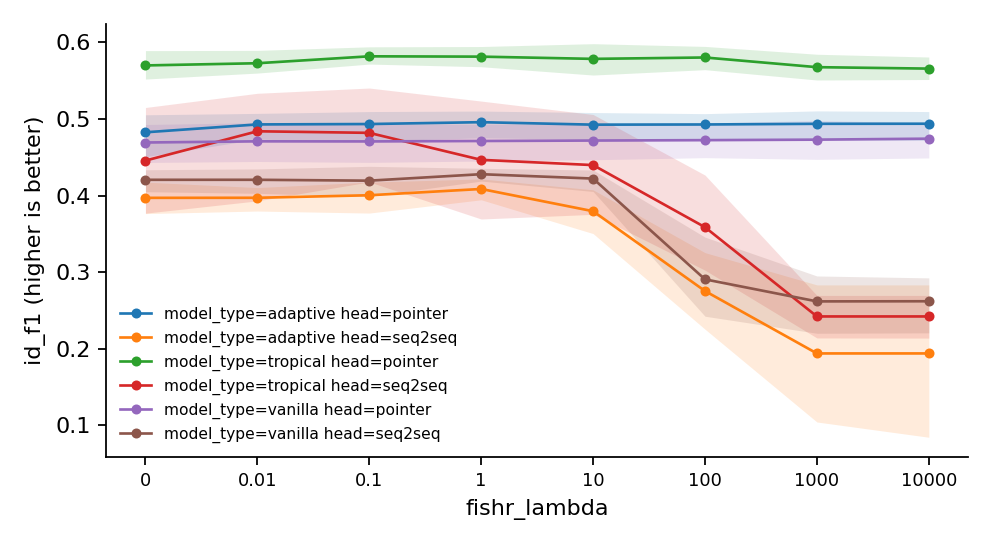
\includegraphics[width=\textwidth]{metric_id_f1.png}
\caption{\texttt{id\_f1} against \texttt{fishr\_lambda}: the mean over seeds with a 95\% bootstrap CI, one line per combination of the other factors.}
\label{fig:id_f1}
\end{figure}

{\small
\begin{longtable}{lllrlrrr}
\caption{\texttt{id\_f1} per cell: mean, 95\% bootstrap CI, SD, seeds, diverged runs.}\label{tab:summary-id_f1}\\
\toprule
\texttt{model\_type} & \texttt{head} & \texttt{fishr\_lambda} & mean & 95\% CI & SD & $n$ & div.\\
\midrule
\endhead
adaptive & pointer & 0 & 0.4827 & [0.451, 0.506] & 0.0356 & 5 & 0\\
adaptive & pointer & 0.01 & 0.493 & [0.474, 0.507] & 0.0226 & 5 & 0\\
adaptive & pointer & 0.1 & 0.4935 & [0.471, 0.51] & 0.0242 & 5 & 0\\
adaptive & pointer & 1 & 0.4959 & [0.475, 0.51] & 0.0235 & 5 & 0\\
adaptive & pointer & 10 & 0.4927 & [0.473, 0.509] & 0.0226 & 5 & 0\\
adaptive & pointer & 100 & 0.4929 & [0.474, 0.507] & 0.0223 & 5 & 0\\
adaptive & pointer & 1000 & 0.4938 & [0.473, 0.511] & 0.024 & 5 & 0\\
adaptive & pointer & 1e+04 & 0.4939 & [0.472, 0.51] & 0.0246 & 5 & 0\\
adaptive & seq2seq & 0 & 0.3971 & [0.377, 0.418] & 0.0277 & 5 & 0\\
adaptive & seq2seq & 0.01 & 0.3972 & [0.38, 0.411] & 0.0207 & 5 & 0\\
adaptive & seq2seq & 0.1 & 0.4005 & [0.377, 0.418] & 0.0266 & 5 & 0\\
adaptive & seq2seq & 1 & 0.4087 & [0.395, 0.422] & 0.018 & 5 & 0\\
adaptive & seq2seq & 10 & 0.3797 & [0.35, 0.408] & 0.038 & 5 & 0\\
adaptive & seq2seq & 100 & 0.2755 & [0.226, 0.326] & 0.0674 & 5 & 0\\
adaptive & seq2seq & 1000 & 0.194 & [0.104, 0.283] & 0.127 & 5 & 0\\
adaptive & seq2seq & 1e+04 & 0.194 & [0.0845, 0.283] & 0.127 & 5 & 0\\
tropical & pointer & 0 & 0.57 & [0.552, 0.589] & 0.0233 & 5 & 0\\
tropical & pointer & 0.01 & 0.5729 & [0.56, 0.59] & 0.0189 & 5 & 0\\
tropical & pointer & 0.1 & 0.5819 & [0.572, 0.594] & 0.0147 & 5 & 0\\
tropical & pointer & 1 & 0.5815 & [0.568, 0.595] & 0.0172 & 5 & 0\\
tropical & pointer & 10 & 0.5786 & [0.557, 0.598] & 0.0268 & 5 & 0\\
tropical & pointer & 100 & 0.5804 & [0.564, 0.595] & 0.0201 & 5 & 0\\
tropical & pointer & 1000 & 0.5678 & [0.551, 0.585] & 0.0216 & 5 & 0\\
tropical & pointer & 1e+04 & 0.5659 & [0.552, 0.581] & 0.0191 & 5 & 0\\
tropical & seq2seq & 0 & 0.4458 & [0.377, 0.515] & 0.0876 & 5 & 0\\
tropical & seq2seq & 0.01 & 0.484 & [0.393, 0.534] & 0.101 & 5 & 0\\
tropical & seq2seq & 0.1 & 0.482 & [0.418, 0.541] & 0.0866 & 5 & 0\\
tropical & seq2seq & 1 & 0.4467 & [0.369, 0.523] & 0.0979 & 5 & 0\\
tropical & seq2seq & 10 & 0.4399 & [0.376, 0.506] & 0.0858 & 5 & 0\\
tropical & seq2seq & 100 & 0.3588 & [0.303, 0.427] & 0.0833 & 5 & 0\\
tropical & seq2seq & 1000 & 0.2423 & [0.214, 0.27] & 0.0357 & 5 & 0\\
tropical & seq2seq & 1e+04 & 0.2423 & [0.214, 0.27] & 0.0357 & 5 & 0\\
vanilla & pointer & 0 & 0.4694 & [0.443, 0.493] & 0.0338 & 5 & 0\\
vanilla & pointer & 0.01 & 0.4709 & [0.445, 0.495] & 0.0319 & 5 & 0\\
vanilla & pointer & 0.1 & 0.4708 & [0.443, 0.494] & 0.0325 & 5 & 0\\
vanilla & pointer & 1 & 0.4714 & [0.445, 0.493] & 0.0315 & 5 & 0\\
vanilla & pointer & 10 & 0.472 & [0.447, 0.494] & 0.0305 & 5 & 0\\
vanilla & pointer & 100 & 0.4725 & [0.45, 0.495] & 0.0325 & 5 & 0\\
vanilla & pointer & 1000 & 0.4731 & [0.447, 0.498] & 0.0324 & 5 & 0\\
vanilla & pointer & 1e+04 & 0.4744 & [0.449, 0.495] & 0.0302 & 5 & 0\\
vanilla & seq2seq & 0 & 0.4207 & [0.405, 0.434] & 0.0185 & 5 & 0\\
vanilla & seq2seq & 0.01 & 0.4207 & [0.403, 0.435] & 0.0205 & 5 & 0\\
vanilla & seq2seq & 0.1 & 0.4196 & [0.399, 0.438] & 0.0249 & 5 & 0\\
vanilla & seq2seq & 1 & 0.428 & [0.419, 0.436] & 0.0113 & 5 & 0\\
vanilla & seq2seq & 10 & 0.4223 & [0.405, 0.433] & 0.019 & 5 & 0\\
vanilla & seq2seq & 100 & 0.2907 & [0.243, 0.346] & 0.0654 & 5 & 0\\
vanilla & seq2seq & 1000 & 0.2619 & [0.22, 0.295] & 0.0471 & 5 & 0\\
vanilla & seq2seq & 1e+04 & 0.2621 & [0.221, 0.293] & 0.0467 & 5 & 0\\
\bottomrule
\end{longtable}
}

{\small
\begin{longtable}{lllrrrl}
\caption{\texttt{id\_f1}: each level of \texttt{fishr\_lambda} against its control (0), within each combination of the other factors. parametric: Dunnett vs control.}\label{tab:control-id_f1}\\
\toprule
\texttt{model\_type} & \texttt{head} & \texttt{fishr\_lambda} & difference & 95\% CI & $p$ & \\
\midrule
\endhead
adaptive & pointer & 0.01 & 0.01027 & [-0.0339, 0.0544] & 0.9809 & \\
adaptive & pointer & 0.1 & 0.01079 & [-0.0334, 0.0549] & 0.9753 & \\
adaptive & pointer & 1 & 0.01321 & [-0.0309, 0.0574] & 0.9341 & \\
adaptive & pointer & 10 & 0.009981 & [-0.0342, 0.0541] & 0.9837 & \\
adaptive & pointer & 100 & 0.01021 & [-0.0339, 0.0544] & 0.9815 & \\
adaptive & pointer & 1000 & 0.01109 & [-0.0331, 0.0552] & 0.9716 & \\
adaptive & pointer & 1e+04 & 0.01121 & [-0.0329, 0.0554] & 0.9700 & \\
adaptive & seq2seq & 0.01 & $8.535\times10^{-5}$ & [-0.124, 0.124] & 1.0000 & \\
adaptive & seq2seq & 0.1 & 0.003383 & [-0.121, 0.127] & 1.0000 & \\
adaptive & seq2seq & 1 & 0.01157 & [-0.113, 0.136] & 0.9999 & \\
adaptive & seq2seq & 10 & -0.01745 & [-0.142, 0.107] & 0.9990 & \\
adaptive & seq2seq & 100 & -0.1217 & [-0.246, 0.00243] & 0.0565 & \\
adaptive & seq2seq & 1000 & -0.2032 & [-0.327, -0.0791] & 0.0005 & *\\
adaptive & seq2seq & 1e+04 & -0.2032 & [-0.327, -0.0791] & 0.0005 & *\\
tropical & pointer & 0.01 & 0.002868 & [-0.033, 0.0387] & 1.0000 & \\
tropical & pointer & 0.1 & 0.01191 & [-0.0239, 0.0477] & 0.8963 & \\
tropical & pointer & 1 & 0.01148 & [-0.0243, 0.0473] & 0.9109 & \\
tropical & pointer & 10 & 0.008564 & [-0.0273, 0.0444] & 0.9780 & \\
tropical & pointer & 100 & 0.01037 & [-0.0255, 0.0462] & 0.9433 & \\
tropical & pointer & 1000 & -0.002257 & [-0.0381, 0.0336] & 1.0000 & \\
tropical & pointer & 1e+04 & -0.004148 & [-0.04, 0.0317] & 0.9997 & \\
tropical & seq2seq & 0.01 & 0.03828 & [-0.102, 0.179] & 0.9577 & \\
tropical & seq2seq & 0.1 & 0.03623 & [-0.104, 0.177] & 0.9678 & \\
tropical & seq2seq & 1 & $9.663\times10^{-4}$ & [-0.14, 0.142] & 1.0000 & \\
tropical & seq2seq & 10 & -0.005852 & [-0.146, 0.135] & 1.0000 & \\
tropical & seq2seq & 100 & -0.08697 & [-0.228, 0.0537] & 0.3852 & \\
tropical & seq2seq & 1000 & -0.2035 & [-0.344, -0.0629] & 0.0022 & *\\
tropical & seq2seq & 1e+04 & -0.2035 & [-0.344, -0.0629] & 0.0022 & *\\
vanilla & pointer & 0.01 & 0.001519 & [-0.0543, 0.0573] & 1.0000 & \\
vanilla & pointer & 0.1 & 0.001406 & [-0.0544, 0.0572] & 1.0000 & \\
vanilla & pointer & 1 & 0.001968 & [-0.0538, 0.0577] & 1.0000 & \\
vanilla & pointer & 10 & 0.002565 & [-0.0532, 0.0583] & 1.0000 & \\
vanilla & pointer & 100 & 0.003075 & [-0.0527, 0.0588] & 1.0000 & \\
vanilla & pointer & 1000 & 0.003735 & [-0.052, 0.0595] & 1.0000 & \\
vanilla & pointer & 1e+04 & 0.00502 & [-0.0508, 0.0608] & 0.9999 & \\
vanilla & seq2seq & 0.01 & $2.937\times10^{-5}$ & [-0.0634, 0.0634] & 1.0000 & \\
vanilla & seq2seq & 0.1 & -0.001136 & [-0.0645, 0.0623] & 1.0000 & \\
vanilla & seq2seq & 1 & 0.007323 & [-0.0561, 0.0707] & 0.9997 & \\
vanilla & seq2seq & 10 & 0.001602 & [-0.0618, 0.065] & 1.0000 & \\
vanilla & seq2seq & 100 & -0.13 & [-0.193, -0.0666] & $<10^{-4}$ & *\\
vanilla & seq2seq & 1000 & -0.1588 & [-0.222, -0.0954] & $<10^{-4}$ & *\\
vanilla & seq2seq & 1e+04 & -0.1586 & [-0.222, -0.0952] & $<10^{-4}$ & *\\
\bottomrule
\end{longtable}
}

{\small
\begin{longtable}{llrrrrr}
\caption{\texttt{id\_f1} against log10 \texttt{fishr\_lambda}: parametric: OLS slope t-test, seed-bootstrap CI, with the Jonckheere--Terpstra ordered-trend $\tau$ and $p$.}\label{tab:trend-id_f1}\\
\toprule
\texttt{model\_type} & \texttt{head} & estimate & 95\% CI & $p$ & JT $\tau$ & JT $p$\\
\midrule
\endhead
adaptive & pointer & $1.475\times10^{-5}$ & [$-3.13\times10^{-4}$, $3.25\times10^{-4}$] & 0.9936 & 0.00952 & 0.9538\\
adaptive & seq2seq & -0.04129 & [-0.0614, -0.0229] & $<10^{-4}$ & -0.629 & 0.0002\\
tropical & pointer & -0.001803 & [-0.00314, $-5.81\times10^{-4}$] & 0.2748 & -0.143 & 0.2851\\
tropical & seq2seq & -0.04617 & [-0.057, -0.0353] & $<10^{-4}$ & -0.632 & 0.0002\\
vanilla & pointer & $5.811\times10^{-4}$ & [$6.45\times10^{-5}$, 0.00117] & 0.8150 & 0.0743 & 0.6007\\
vanilla & seq2seq & -0.03316 & [-0.0393, -0.0273] & $<10^{-4}$ & -0.592 & 0.0002\\
\bottomrule
\end{longtable}
}

{\small
\begin{longtable}{lrrrl}
\caption{\texttt{id\_f1}: paired contrasts by seed, Holm-corrected across the cells. parametric: paired t-test by seed, Holm.}\label{tab:paired-id_f1}\\
\toprule
contrast (within) & difference & 95\% CI & $p$ & \\
\midrule
\endhead
\stackcell{model\_type: tropical - vanilla\\\footnotesize head=pointer fishr\_lambda=0 } & 0.1006 & [0.0562, 0.145] & 0.0301 & *\\
\stackcell{model\_type: tropical - vanilla\\\footnotesize head=pointer fishr\_lambda=0.01 } & 0.102 & [0.059, 0.145] & 0.0301 & *\\
\stackcell{model\_type: tropical - vanilla\\\footnotesize head=pointer fishr\_lambda=0.1 } & 0.1111 & [0.0699, 0.152] & 0.0256 & *\\
\stackcell{model\_type: tropical - vanilla\\\footnotesize head=pointer fishr\_lambda=1 } & 0.1101 & [0.0638, 0.157] & 0.0301 & *\\
\stackcell{model\_type: tropical - vanilla\\\footnotesize head=pointer fishr\_lambda=10 } & 0.1066 & [0.066, 0.147] & 0.0265 & *\\
\stackcell{model\_type: tropical - vanilla\\\footnotesize head=pointer fishr\_lambda=100 } & 0.1079 & [0.0689, 0.147] & 0.0247 & *\\
\stackcell{model\_type: tropical - vanilla\\\footnotesize head=pointer fishr\_lambda=1000 } & 0.09464 & [0.0584, 0.131] & 0.0265 & *\\
\stackcell{model\_type: tropical - vanilla\\\footnotesize head=pointer fishr\_lambda=1e+04 } & 0.09146 & [0.0565, 0.126] & 0.0265 & *\\
\stackcell{model\_type: tropical - vanilla\\\footnotesize head=seq2seq fishr\_lambda=0 } & 0.02507 & [-0.0985, 0.149] & 1.0000 & \\
\stackcell{model\_type: tropical - vanilla\\\footnotesize head=seq2seq fishr\_lambda=0.01 } & 0.06333 & [-0.0603, 0.187] & 1.0000 & \\
\stackcell{model\_type: tropical - vanilla\\\footnotesize head=seq2seq fishr\_lambda=0.1 } & 0.06244 & [-0.0586, 0.183] & 1.0000 & \\
\stackcell{model\_type: tropical - vanilla\\\footnotesize head=seq2seq fishr\_lambda=1 } & 0.01872 & [-0.11, 0.148] & 1.0000 & \\
\stackcell{model\_type: tropical - vanilla\\\footnotesize head=seq2seq fishr\_lambda=10 } & 0.01762 & [-0.097, 0.132] & 1.0000 & \\
\stackcell{model\_type: tropical - vanilla\\\footnotesize head=seq2seq fishr\_lambda=100 } & 0.06808 & [-0.0664, 0.203] & 1.0000 & \\
\stackcell{model\_type: tropical - vanilla\\\footnotesize head=seq2seq fishr\_lambda=1000 } & -0.01966 & [-0.0849, 0.0455] & 1.0000 & \\
\stackcell{model\_type: tropical - vanilla\\\footnotesize head=seq2seq fishr\_lambda=1e+04 } & -0.01984 & [-0.0848, 0.0451] & 1.0000 & \\
\stackcell{model\_type: adaptive - vanilla\\\footnotesize head=pointer fishr\_lambda=0 } & 0.01332 & [-0.00744, 0.0341] & 0.5977 & \\
\stackcell{model\_type: adaptive - vanilla\\\footnotesize head=pointer fishr\_lambda=0.01 } & 0.02208 & [0.00321, 0.0409] & 0.3140 & \\
\stackcell{model\_type: adaptive - vanilla\\\footnotesize head=pointer fishr\_lambda=0.1 } & 0.02271 & [0.00628, 0.0391] & 0.2403 & \\
\stackcell{model\_type: adaptive - vanilla\\\footnotesize head=pointer fishr\_lambda=1 } & 0.02457 & [0.00746, 0.0417] & 0.2280 & \\
\stackcell{model\_type: adaptive - vanilla\\\footnotesize head=pointer fishr\_lambda=10 } & 0.02074 & [0.00451, 0.037] & 0.2621 & \\
\stackcell{model\_type: adaptive - vanilla\\\footnotesize head=pointer fishr\_lambda=100 } & 0.02046 & [$-5.88\times10^{-4}$, 0.0415] & 0.3791 & \\
\stackcell{model\_type: adaptive - vanilla\\\footnotesize head=pointer fishr\_lambda=1000 } & 0.02068 & [0.00187, 0.0395] & 0.3360 & \\
\stackcell{model\_type: adaptive - vanilla\\\footnotesize head=pointer fishr\_lambda=1e+04 } & 0.01952 & [0.00488, 0.0341] & 0.2494 & \\
\stackcell{model\_type: adaptive - vanilla\\\footnotesize head=seq2seq fishr\_lambda=0 } & -0.02356 & [-0.0381, -0.00899] & 0.1638 & \\
\stackcell{model\_type: adaptive - vanilla\\\footnotesize head=seq2seq fishr\_lambda=0.01 } & -0.0235 & [-0.0322, -0.0148] & 0.0269 & *\\
\stackcell{model\_type: adaptive - vanilla\\\footnotesize head=seq2seq fishr\_lambda=0.1 } & -0.01904 & [-0.0363, -0.00182] & 0.3360 & \\
\stackcell{model\_type: adaptive - vanilla\\\footnotesize head=seq2seq fishr\_lambda=1 } & -0.01931 & [-0.0426, 0.00394] & 0.4121 & \\
\stackcell{model\_type: adaptive - vanilla\\\footnotesize head=seq2seq fishr\_lambda=10 } & -0.04261 & [-0.0894, 0.00421] & 0.3894 & \\
\stackcell{model\_type: adaptive - vanilla\\\footnotesize head=seq2seq fishr\_lambda=100 } & -0.01524 & [-0.16, 0.13] & 0.7850 & \\
\stackcell{model\_type: adaptive - vanilla\\\footnotesize head=seq2seq fishr\_lambda=1000 } & -0.06795 & [-0.199, 0.0626] & 0.6657 & \\
\stackcell{model\_type: adaptive - vanilla\\\footnotesize head=seq2seq fishr\_lambda=1e+04 } & -0.06813 & [-0.199, 0.0628] & 0.6657 & \\
\stackcell{head: pointer - seq2seq\\\footnotesize model\_type=adaptive fishr\_lambda=0 } & 0.08558 & [0.0196, 0.152] & 0.2276 & \\
\stackcell{head: pointer - seq2seq\\\footnotesize model\_type=adaptive fishr\_lambda=0.01 } & 0.09577 & [0.049, 0.143] & 0.0852 & \\
\stackcell{head: pointer - seq2seq\\\footnotesize model\_type=adaptive fishr\_lambda=0.1 } & 0.09299 & [0.0391, 0.147] & 0.1129 & \\
\stackcell{head: pointer - seq2seq\\\footnotesize model\_type=adaptive fishr\_lambda=1 } & 0.08722 & [0.055, 0.119] & 0.0353 & *\\
\stackcell{head: pointer - seq2seq\\\footnotesize model\_type=adaptive fishr\_lambda=10 } & 0.113 & [0.0505, 0.176] & 0.1036 & \\
\stackcell{head: pointer - seq2seq\\\footnotesize model\_type=adaptive fishr\_lambda=100 } & 0.2175 & [0.144, 0.291] & 0.0270 & *\\
\stackcell{head: pointer - seq2seq\\\footnotesize model\_type=adaptive fishr\_lambda=1000 } & 0.2998 & [0.148, 0.451] & 0.0869 & \\
\stackcell{head: pointer - seq2seq\\\footnotesize model\_type=adaptive fishr\_lambda=1e+04 } & 0.3 & [0.15, 0.45] & 0.0869 & \\
\stackcell{head: pointer - seq2seq\\\footnotesize model\_type=tropical fishr\_lambda=0 } & 0.1243 & [0.0283, 0.22] & 0.2276 & \\
\stackcell{head: pointer - seq2seq\\\footnotesize model\_type=tropical fishr\_lambda=0.01 } & 0.08884 & [-0.0261, 0.204] & 0.3177 & \\
\stackcell{head: pointer - seq2seq\\\footnotesize model\_type=tropical fishr\_lambda=0.1 } & 0.09994 & [-0.00806, 0.208] & 0.3102 & \\
\stackcell{head: pointer - seq2seq\\\footnotesize model\_type=tropical fishr\_lambda=1 } & 0.1348 & [0.0204, 0.249] & 0.2276 & \\
\stackcell{head: pointer - seq2seq\\\footnotesize model\_type=tropical fishr\_lambda=10 } & 0.1387 & [0.0418, 0.236] & 0.1814 & \\
\stackcell{head: pointer - seq2seq\\\footnotesize model\_type=tropical fishr\_lambda=100 } & 0.2216 & [0.109, 0.334] & 0.0869 & \\
\stackcell{head: pointer - seq2seq\\\footnotesize model\_type=tropical fishr\_lambda=1000 } & 0.3255 & [0.285, 0.366] & 0.0006 & *\\
\stackcell{head: pointer - seq2seq\\\footnotesize model\_type=tropical fishr\_lambda=1e+04 } & 0.3236 & [0.282, 0.365] & 0.0006 & *\\
\stackcell{head: pointer - seq2seq\\\footnotesize model\_type=vanilla fishr\_lambda=0 } & 0.0487 & [-0.0127, 0.11] & 0.3177 & \\
\stackcell{head: pointer - seq2seq\\\footnotesize model\_type=vanilla fishr\_lambda=0.01 } & 0.05019 & [-0.00938, 0.11] & 0.3177 & \\
\stackcell{head: pointer - seq2seq\\\footnotesize model\_type=vanilla fishr\_lambda=0.1 } & 0.05124 & [-0.00986, 0.112] & 0.3177 & \\
\stackcell{head: pointer - seq2seq\\\footnotesize model\_type=vanilla fishr\_lambda=1 } & 0.04334 & [$-2.04\times10^{-4}$, 0.0869] & 0.3040 & \\
\stackcell{head: pointer - seq2seq\\\footnotesize model\_type=vanilla fishr\_lambda=10 } & 0.04966 & [0.00879, 0.0905] & 0.2276 & \\
\stackcell{head: pointer - seq2seq\\\footnotesize model\_type=vanilla fishr\_lambda=100 } & 0.1818 & [0.0763, 0.287] & 0.1129 & \\
\stackcell{head: pointer - seq2seq\\\footnotesize model\_type=vanilla fishr\_lambda=1000 } & 0.2112 & [0.132, 0.291] & 0.0353 & *\\
\stackcell{head: pointer - seq2seq\\\footnotesize model\_type=vanilla fishr\_lambda=1e+04 } & 0.2123 & [0.133, 0.291] & 0.0353 & *\\
\bottomrule
\end{longtable}
}

\subsection{\texttt{id\_exact}}
\begin{figure}[tbp]
\centering
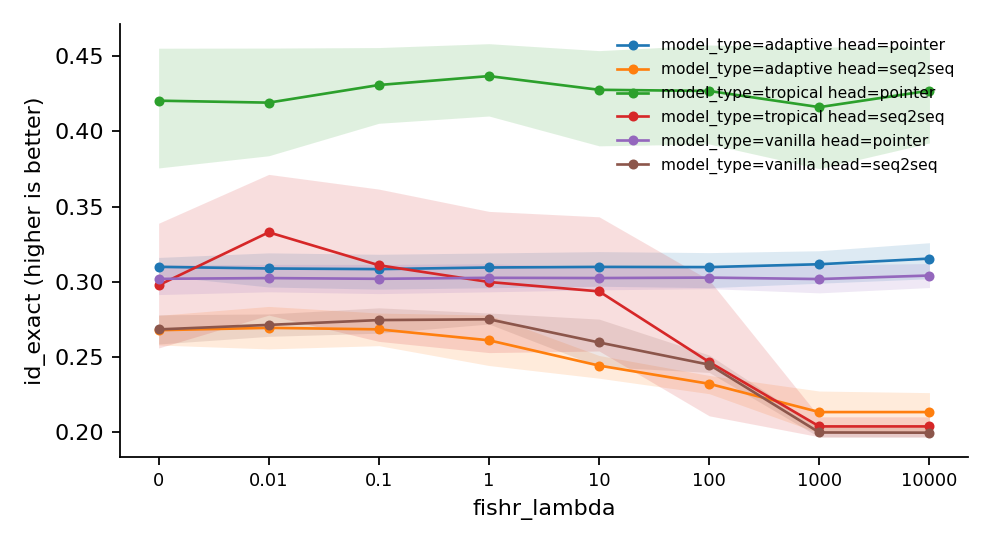
\includegraphics[width=\textwidth]{metric_id_exact.png}
\caption{\texttt{id\_exact} against \texttt{fishr\_lambda}: the mean over seeds with a 95\% bootstrap CI, one line per combination of the other factors.}
\label{fig:id_exact}
\end{figure}

{\small
\begin{longtable}{lllrlrrr}
\caption{\texttt{id\_exact} per cell: mean, 95\% bootstrap CI, SD, seeds, diverged runs.}\label{tab:summary-id_exact}\\
\toprule
\texttt{model\_type} & \texttt{head} & \texttt{fishr\_lambda} & mean & 95\% CI & SD & $n$ & div.\\
\midrule
\endhead
adaptive & pointer & 0 & 0.3099 & [0.304, 0.316] & 0.00807 & 5 & 0\\
adaptive & pointer & 0.01 & 0.3088 & [0.297, 0.319] & 0.0149 & 5 & 0\\
adaptive & pointer & 0.1 & 0.3084 & [0.295, 0.318] & 0.0153 & 5 & 0\\
adaptive & pointer & 1 & 0.3095 & [0.296, 0.319] & 0.0155 & 5 & 0\\
adaptive & pointer & 10 & 0.3099 & [0.297, 0.32] & 0.0155 & 5 & 0\\
adaptive & pointer & 100 & 0.3098 & [0.296, 0.319] & 0.0154 & 5 & 0\\
adaptive & pointer & 1000 & 0.3117 & [0.299, 0.321] & 0.0147 & 5 & 0\\
adaptive & pointer & 1e+04 & 0.3154 & [0.302, 0.326] & 0.016 & 5 & 0\\
adaptive & seq2seq & 0 & 0.2678 & [0.258, 0.278] & 0.0133 & 5 & 0\\
adaptive & seq2seq & 0.01 & 0.2694 & [0.255, 0.284] & 0.0178 & 5 & 0\\
adaptive & seq2seq & 0.1 & 0.2684 & [0.258, 0.279] & 0.0147 & 5 & 0\\
adaptive & seq2seq & 1 & 0.2611 & [0.244, 0.278] & 0.0219 & 5 & 0\\
adaptive & seq2seq & 10 & 0.2443 & [0.236, 0.251] & 0.00991 & 5 & 0\\
adaptive & seq2seq & 100 & 0.2322 & [0.226, 0.238] & 0.00799 & 5 & 0\\
adaptive & seq2seq & 1000 & 0.2134 & [0.199, 0.227] & 0.0178 & 5 & 0\\
adaptive & seq2seq & 1e+04 & 0.2134 & [0.199, 0.226] & 0.0178 & 5 & 0\\
tropical & pointer & 0 & 0.4204 & [0.376, 0.455] & 0.052 & 5 & 0\\
tropical & pointer & 0.01 & 0.4191 & [0.384, 0.455] & 0.0465 & 5 & 0\\
tropical & pointer & 0.1 & 0.4308 & [0.405, 0.456] & 0.0337 & 5 & 0\\
tropical & pointer & 1 & 0.4368 & [0.41, 0.458] & 0.032 & 5 & 0\\
tropical & pointer & 10 & 0.4276 & [0.39, 0.454] & 0.0415 & 5 & 0\\
tropical & pointer & 100 & 0.4269 & [0.392, 0.457] & 0.0427 & 5 & 0\\
tropical & pointer & 1000 & 0.4161 & [0.375, 0.456] & 0.0545 & 5 & 0\\
tropical & pointer & 1e+04 & 0.4271 & [0.392, 0.457] & 0.0426 & 5 & 0\\
tropical & seq2seq & 0 & 0.2977 & [0.256, 0.339] & 0.0557 & 5 & 0\\
tropical & seq2seq & 0.01 & 0.3329 & [0.278, 0.371] & 0.0611 & 5 & 0\\
tropical & seq2seq & 0.1 & 0.311 & [0.26, 0.362] & 0.0659 & 5 & 0\\
tropical & seq2seq & 1 & 0.2999 & [0.253, 0.347] & 0.0615 & 5 & 0\\
tropical & seq2seq & 10 & 0.2936 & [0.254, 0.343] & 0.0579 & 5 & 0\\
tropical & seq2seq & 100 & 0.2466 & [0.211, 0.301] & 0.0618 & 5 & 0\\
tropical & seq2seq & 1000 & 0.2038 & [0.197, 0.21] & 0.00849 & 5 & 0\\
tropical & seq2seq & 1e+04 & 0.2038 & [0.197, 0.21] & 0.00849 & 5 & 0\\
vanilla & pointer & 0 & 0.302 & [0.291, 0.311] & 0.013 & 5 & 0\\
vanilla & pointer & 0.01 & 0.3025 & [0.293, 0.312] & 0.0122 & 5 & 0\\
vanilla & pointer & 0.1 & 0.302 & [0.292, 0.312] & 0.0125 & 5 & 0\\
vanilla & pointer & 1 & 0.3026 & [0.293, 0.312] & 0.0123 & 5 & 0\\
vanilla & pointer & 10 & 0.3025 & [0.295, 0.31] & 0.0097 & 5 & 0\\
vanilla & pointer & 100 & 0.3028 & [0.295, 0.31] & 0.00994 & 5 & 0\\
vanilla & pointer & 1000 & 0.3018 & [0.293, 0.311] & 0.0121 & 5 & 0\\
vanilla & pointer & 1e+04 & 0.3042 & [0.296, 0.312] & 0.0109 & 5 & 0\\
vanilla & seq2seq & 0 & 0.2683 & [0.259, 0.278] & 0.0124 & 5 & 0\\
vanilla & seq2seq & 0.01 & 0.2713 & [0.264, 0.279] & 0.0102 & 5 & 0\\
vanilla & seq2seq & 0.1 & 0.2745 & [0.266, 0.283] & 0.0111 & 5 & 0\\
vanilla & seq2seq & 1 & 0.2751 & [0.272, 0.279] & 0.00466 & 5 & 0\\
vanilla & seq2seq & 10 & 0.2597 & [0.244, 0.275] & 0.0196 & 5 & 0\\
vanilla & seq2seq & 100 & 0.2449 & [0.24, 0.251] & 0.00771 & 5 & 0\\
vanilla & seq2seq & 1000 & 0.1998 & [0.197, 0.203] & 0.00435 & 5 & 0\\
vanilla & seq2seq & 1e+04 & 0.1997 & [0.197, 0.203] & 0.00422 & 5 & 0\\
\bottomrule
\end{longtable}
}

{\small
\begin{longtable}{lllrrrl}
\caption{\texttt{id\_exact}: each level of \texttt{fishr\_lambda} against its control (0), within each combination of the other factors. parametric: Dunnett vs control.}\label{tab:control-id_exact}\\
\toprule
\texttt{model\_type} & \texttt{head} & \texttt{fishr\_lambda} & difference & 95\% CI & $p$ & \\
\midrule
\endhead
adaptive & pointer & 0.01 & -0.0011 & [-0.0266, 0.0244] & 1.0000 & \\
adaptive & pointer & 0.1 & -0.00152 & [-0.0271, 0.024] & 1.0000 & \\
adaptive & pointer & 1 & $-4.400\times10^{-4}$ & [-0.026, 0.0251] & 1.0000 & \\
adaptive & pointer & 10 & $-4.000\times10^{-5}$ & [-0.0256, 0.0255] & 1.0000 & \\
adaptive & pointer & 100 & $-1.800\times10^{-4}$ & [-0.0257, 0.0254] & 1.0000 & \\
adaptive & pointer & 1000 & 0.00172 & [-0.0238, 0.0273] & 1.0000 & \\
adaptive & pointer & 1e+04 & 0.00548 & [-0.0201, 0.031] & 0.9877 & \\
adaptive & seq2seq & 0.01 & 0.00156 & [-0.026, 0.0291] & 1.0000 & \\
adaptive & seq2seq & 0.1 & $5.600\times10^{-4}$ & [-0.027, 0.0281] & 1.0000 & \\
adaptive & seq2seq & 1 & -0.00672 & [-0.0342, 0.0208] & 0.9754 & \\
adaptive & seq2seq & 10 & -0.02354 & [-0.0511, 0.00397] & 0.1186 & \\
adaptive & seq2seq & 100 & -0.03564 & [-0.0632, -0.00813] & 0.0067 & *\\
adaptive & seq2seq & 1000 & -0.05444 & [-0.082, -0.0269] & $<10^{-4}$ & *\\
adaptive & seq2seq & 1e+04 & -0.05444 & [-0.082, -0.0269] & $<10^{-4}$ & *\\
tropical & pointer & 0.01 & -0.0013 & [-0.0778, 0.0752] & 1.0000 & \\
tropical & pointer & 0.1 & 0.01042 & [-0.0661, 0.087] & 0.9992 & \\
tropical & pointer & 1 & 0.01636 & [-0.0602, 0.0929] & 0.9880 & \\
tropical & pointer & 10 & 0.00724 & [-0.0693, 0.0838] & 0.9999 & \\
tropical & pointer & 100 & 0.00646 & [-0.0701, 0.083] & 1.0000 & \\
tropical & pointer & 1000 & -0.0043 & [-0.0808, 0.0722] & 1.0000 & \\
tropical & pointer & 1e+04 & 0.00668 & [-0.0699, 0.0832] & 1.0000 & \\
tropical & seq2seq & 0.01 & 0.03518 & [-0.057, 0.127] & 0.8231 & \\
tropical & seq2seq & 0.1 & 0.01328 & [-0.0789, 0.105] & 0.9988 & \\
tropical & seq2seq & 1 & 0.00214 & [-0.09, 0.0943] & 1.0000 & \\
tropical & seq2seq & 10 & -0.0041 & [-0.0963, 0.0881] & 1.0000 & \\
tropical & seq2seq & 100 & -0.05108 & [-0.143, 0.0411] & 0.4972 & \\
tropical & seq2seq & 1000 & -0.09388 & [-0.186, -0.00172] & 0.0444 & *\\
tropical & seq2seq & 1e+04 & -0.09388 & [-0.186, -0.00172] & 0.0445 & *\\
vanilla & pointer & 0.01 & $4.800\times10^{-4}$ & [-0.0198, 0.0208] & 1.0000 & \\
vanilla & pointer & 0.1 & 0 & [-0.0203, 0.0203] & 1.0000 & \\
vanilla & pointer & 1 & $6.600\times10^{-4}$ & [-0.0196, 0.021] & 1.0000 & \\
vanilla & pointer & 10 & $5.000\times10^{-4}$ & [-0.0198, 0.0208] & 1.0000 & \\
vanilla & pointer & 100 & $8.000\times10^{-4}$ & [-0.0195, 0.0211] & 1.0000 & \\
vanilla & pointer & 1000 & $-1.600\times10^{-4}$ & [-0.0205, 0.0201] & 1.0000 & \\
vanilla & pointer & 1e+04 & 0.00218 & [-0.0181, 0.0225] & 0.9998 & \\
vanilla & seq2seq & 0.01 & 0.003 & [-0.0154, 0.0214] & 0.9975 & \\
vanilla & seq2seq & 0.1 & 0.0062 & [-0.0122, 0.0246] & 0.8891 & \\
vanilla & seq2seq & 1 & 0.00672 & [-0.0116, 0.0251] & 0.8481 & \\
vanilla & seq2seq & 10 & -0.00868 & [-0.027, 0.00967] & 0.6542 & \\
vanilla & seq2seq & 100 & -0.02344 & [-0.0418, -0.00509] & 0.0076 & *\\
vanilla & seq2seq & 1000 & -0.06852 & [-0.0869, -0.0502] & $<10^{-4}$ & *\\
vanilla & seq2seq & 1e+04 & -0.06866 & [-0.087, -0.0503] & $<10^{-4}$ & *\\
\bottomrule
\end{longtable}
}

{\small
\begin{longtable}{llrrrrr}
\caption{\texttt{id\_exact} against log10 \texttt{fishr\_lambda}: parametric: OLS slope t-test, seed-bootstrap CI, with the Jonckheere--Terpstra ordered-trend $\tau$ and $p$.}\label{tab:trend-id_exact}\\
\toprule
\texttt{model\_type} & \texttt{head} & estimate & 95\% CI & $p$ & JT $\tau$ & JT $p$\\
\midrule
\endhead
adaptive & pointer & $9.457\times10^{-4}$ & [$8.07\times10^{-4}$, 0.00109] & 0.4354 & 0.19 & 0.1562\\
adaptive & seq2seq & -0.01096 & [-0.016, -0.00587] & $<10^{-4}$ & -0.728 & 0.0002\\
tropical & pointer & $-5.500\times10^{-4}$ & [-0.00223, $4.64\times10^{-4}$] & 0.8708 & 0.0114 & 0.9368\\
tropical & seq2seq & -0.02338 & [-0.0308, -0.0146] & $<10^{-4}$ & -0.615 & 0.0002\\
vanilla & pointer & $1.757\times10^{-4}$ & [$-4.41\times10^{-4}$, $7.52\times10^{-4}$] & 0.8448 & 0.0381 & 0.7908\\
vanilla & seq2seq & -0.01409 & [-0.0158, -0.0124] & $<10^{-4}$ & -0.686 & 0.0002\\
\bottomrule
\end{longtable}
}

{\small
\begin{longtable}{lrrrl}
\caption{\texttt{id\_exact}: paired contrasts by seed, Holm-corrected across the cells. parametric: paired t-test by seed, Holm.}\label{tab:paired-id_exact}\\
\toprule
contrast (within) & difference & 95\% CI & $p$ & \\
\midrule
\endhead
\stackcell{model\_type: tropical - vanilla\\\footnotesize head=pointer fishr\_lambda=0 } & 0.1184 & [0.0672, 0.17] & 0.0303 & *\\
\stackcell{model\_type: tropical - vanilla\\\footnotesize head=pointer fishr\_lambda=0.01 } & 0.1166 & [0.0733, 0.16] & 0.0188 & *\\
\stackcell{model\_type: tropical - vanilla\\\footnotesize head=pointer fishr\_lambda=0.1 } & 0.1288 & [0.0996, 0.158] & 0.0038 & *\\
\stackcell{model\_type: tropical - vanilla\\\footnotesize head=pointer fishr\_lambda=1 } & 0.1341 & [0.106, 0.162] & 0.0030 & *\\
\stackcell{model\_type: tropical - vanilla\\\footnotesize head=pointer fishr\_lambda=10 } & 0.1252 & [0.0844, 0.166] & 0.0142 & *\\
\stackcell{model\_type: tropical - vanilla\\\footnotesize head=pointer fishr\_lambda=100 } & 0.1241 & [0.0819, 0.166] & 0.0147 & *\\
\stackcell{model\_type: tropical - vanilla\\\footnotesize head=pointer fishr\_lambda=1000 } & 0.1143 & [0.0611, 0.167] & 0.0357 & *\\
\stackcell{model\_type: tropical - vanilla\\\footnotesize head=pointer fishr\_lambda=1e+04 } & 0.1229 & [0.0831, 0.163] & 0.0142 & *\\
\stackcell{model\_type: tropical - vanilla\\\footnotesize head=seq2seq fishr\_lambda=0 } & 0.02938 & [-0.048, 0.107] & 1.0000 & \\
\stackcell{model\_type: tropical - vanilla\\\footnotesize head=seq2seq fishr\_lambda=0.01 } & 0.06156 & [-0.014, 0.137] & 0.6919 & \\
\stackcell{model\_type: tropical - vanilla\\\footnotesize head=seq2seq fishr\_lambda=0.1 } & 0.03646 & [-0.0556, 0.129] & 1.0000 & \\
\stackcell{model\_type: tropical - vanilla\\\footnotesize head=seq2seq fishr\_lambda=1 } & 0.0248 & [-0.0543, 0.104] & 1.0000 & \\
\stackcell{model\_type: tropical - vanilla\\\footnotesize head=seq2seq fishr\_lambda=10 } & 0.03396 & [-0.0289, 0.0968] & 1.0000 & \\
\stackcell{model\_type: tropical - vanilla\\\footnotesize head=seq2seq fishr\_lambda=100 } & 0.00174 & [-0.0758, 0.0793] & 1.0000 & \\
\stackcell{model\_type: tropical - vanilla\\\footnotesize head=seq2seq fishr\_lambda=1000 } & 0.00402 & [-0.0106, 0.0186] & 1.0000 & \\
\stackcell{model\_type: tropical - vanilla\\\footnotesize head=seq2seq fishr\_lambda=1e+04 } & 0.00416 & [-0.0104, 0.0188] & 1.0000 & \\
\stackcell{model\_type: adaptive - vanilla\\\footnotesize head=pointer fishr\_lambda=0 } & 0.00796 & [-0.00553, 0.0214] & 1.0000 & \\
\stackcell{model\_type: adaptive - vanilla\\\footnotesize head=pointer fishr\_lambda=0.01 } & 0.00638 & [-0.00642, 0.0192] & 1.0000 & \\
\stackcell{model\_type: adaptive - vanilla\\\footnotesize head=pointer fishr\_lambda=0.1 } & 0.00644 & [-0.00322, 0.0161] & 1.0000 & \\
\stackcell{model\_type: adaptive - vanilla\\\footnotesize head=pointer fishr\_lambda=1 } & 0.00686 & [-0.00574, 0.0195] & 1.0000 & \\
\stackcell{model\_type: adaptive - vanilla\\\footnotesize head=pointer fishr\_lambda=10 } & 0.00742 & [-0.00395, 0.0188] & 1.0000 & \\
\stackcell{model\_type: adaptive - vanilla\\\footnotesize head=pointer fishr\_lambda=100 } & 0.00698 & [-0.00518, 0.0191] & 1.0000 & \\
\stackcell{model\_type: adaptive - vanilla\\\footnotesize head=pointer fishr\_lambda=1000 } & 0.00984 & [$7.68\times10^{-4}$, 0.0189] & 0.6114 & \\
\stackcell{model\_type: adaptive - vanilla\\\footnotesize head=pointer fishr\_lambda=1e+04 } & 0.01126 & [$-7.85\times10^{-4}$, 0.0233] & 0.8447 & \\
\stackcell{model\_type: adaptive - vanilla\\\footnotesize head=seq2seq fishr\_lambda=0 } & $-5.200\times10^{-4}$ & [-0.00745, 0.00641] & 1.0000 & \\
\stackcell{model\_type: adaptive - vanilla\\\footnotesize head=seq2seq fishr\_lambda=0.01 } & -0.00196 & [-0.0141, 0.0102] & 1.0000 & \\
\stackcell{model\_type: adaptive - vanilla\\\footnotesize head=seq2seq fishr\_lambda=0.1 } & -0.00616 & [-0.016, 0.00365] & 1.0000 & \\
\stackcell{model\_type: adaptive - vanilla\\\footnotesize head=seq2seq fishr\_lambda=1 } & -0.01396 & [-0.0363, 0.00833] & 1.0000 & \\
\stackcell{model\_type: adaptive - vanilla\\\footnotesize head=seq2seq fishr\_lambda=10 } & -0.01538 & [-0.0447, 0.0139] & 1.0000 & \\
\stackcell{model\_type: adaptive - vanilla\\\footnotesize head=seq2seq fishr\_lambda=100 } & -0.01272 & [-0.0243, -0.00112] & 0.6114 & \\
\stackcell{model\_type: adaptive - vanilla\\\footnotesize head=seq2seq fishr\_lambda=1000 } & 0.01356 & [-0.00667, 0.0338] & 1.0000 & \\
\stackcell{model\_type: adaptive - vanilla\\\footnotesize head=seq2seq fishr\_lambda=1e+04 } & 0.0137 & [-0.00678, 0.0342] & 1.0000 & \\
\stackcell{head: pointer - seq2seq\\\footnotesize model\_type=adaptive fishr\_lambda=0 } & 0.04212 & [0.0217, 0.0625] & 0.0621 & \\
\stackcell{head: pointer - seq2seq\\\footnotesize model\_type=adaptive fishr\_lambda=0.01 } & 0.03946 & [0.0143, 0.0647] & 0.0670 & \\
\stackcell{head: pointer - seq2seq\\\footnotesize model\_type=adaptive fishr\_lambda=0.1 } & 0.04004 & [0.0124, 0.0676] & 0.0670 & \\
\stackcell{head: pointer - seq2seq\\\footnotesize model\_type=adaptive fishr\_lambda=1 } & 0.0484 & [0.0216, 0.0752] & 0.0670 & \\
\stackcell{head: pointer - seq2seq\\\footnotesize model\_type=adaptive fishr\_lambda=10 } & 0.06562 & [0.0435, 0.0878] & 0.0190 & *\\
\stackcell{head: pointer - seq2seq\\\footnotesize model\_type=adaptive fishr\_lambda=100 } & 0.07758 & [0.0586, 0.0966] & 0.0069 & *\\
\stackcell{head: pointer - seq2seq\\\footnotesize model\_type=adaptive fishr\_lambda=1000 } & 0.09828 & [0.0703, 0.126] & 0.0112 & *\\
\stackcell{head: pointer - seq2seq\\\footnotesize model\_type=adaptive fishr\_lambda=1e+04 } & 0.102 & [0.0743, 0.13] & 0.0099 & *\\
\stackcell{head: pointer - seq2seq\\\footnotesize model\_type=tropical fishr\_lambda=0 } & 0.1227 & [0.0454, 0.2] & 0.0670 & \\
\stackcell{head: pointer - seq2seq\\\footnotesize model\_type=tropical fishr\_lambda=0.01 } & 0.0862 & [0.036, 0.136] & 0.0670 & \\
\stackcell{head: pointer - seq2seq\\\footnotesize model\_type=tropical fishr\_lambda=0.1 } & 0.1198 & [0.0235, 0.216] & 0.0670 & \\
\stackcell{head: pointer - seq2seq\\\footnotesize model\_type=tropical fishr\_lambda=1 } & 0.1369 & [0.0712, 0.203] & 0.0621 & \\
\stackcell{head: pointer - seq2seq\\\footnotesize model\_type=tropical fishr\_lambda=10 } & 0.134 & [0.0662, 0.202] & 0.0621 & \\
\stackcell{head: pointer - seq2seq\\\footnotesize model\_type=tropical fishr\_lambda=100 } & 0.1802 & [0.091, 0.269] & 0.0621 & \\
\stackcell{head: pointer - seq2seq\\\footnotesize model\_type=tropical fishr\_lambda=1000 } & 0.2123 & [0.149, 0.276] & 0.0127 & *\\
\stackcell{head: pointer - seq2seq\\\footnotesize model\_type=tropical fishr\_lambda=1e+04 } & 0.2232 & [0.175, 0.271] & 0.0043 & *\\
\stackcell{head: pointer - seq2seq\\\footnotesize model\_type=vanilla fishr\_lambda=0 } & 0.03364 & [0.0186, 0.0487] & 0.0517 & \\
\stackcell{head: pointer - seq2seq\\\footnotesize model\_type=vanilla fishr\_lambda=0.01 } & 0.03112 & [0.0125, 0.0497] & 0.0670 & \\
\stackcell{head: pointer - seq2seq\\\footnotesize model\_type=vanilla fishr\_lambda=0.1 } & 0.02744 & [0.00525, 0.0496] & 0.0670 & \\
\stackcell{head: pointer - seq2seq\\\footnotesize model\_type=vanilla fishr\_lambda=1 } & 0.02758 & [0.0118, 0.0433] & 0.0670 & \\
\stackcell{head: pointer - seq2seq\\\footnotesize model\_type=vanilla fishr\_lambda=10 } & 0.04282 & [0.0218, 0.0638] & 0.0621 & \\
\stackcell{head: pointer - seq2seq\\\footnotesize model\_type=vanilla fishr\_lambda=100 } & 0.05788 & [0.0484, 0.0673] & 0.0017 & *\\
\stackcell{head: pointer - seq2seq\\\footnotesize model\_type=vanilla fishr\_lambda=1000 } & 0.102 & [0.0818, 0.122] & 0.0033 & *\\
\stackcell{head: pointer - seq2seq\\\footnotesize model\_type=vanilla fishr\_lambda=1e+04 } & 0.1045 & [0.086, 0.123] & 0.0022 & *\\
\bottomrule
\end{longtable}
}


\section{Curves}
\begin{figure}[tbp]
\centering
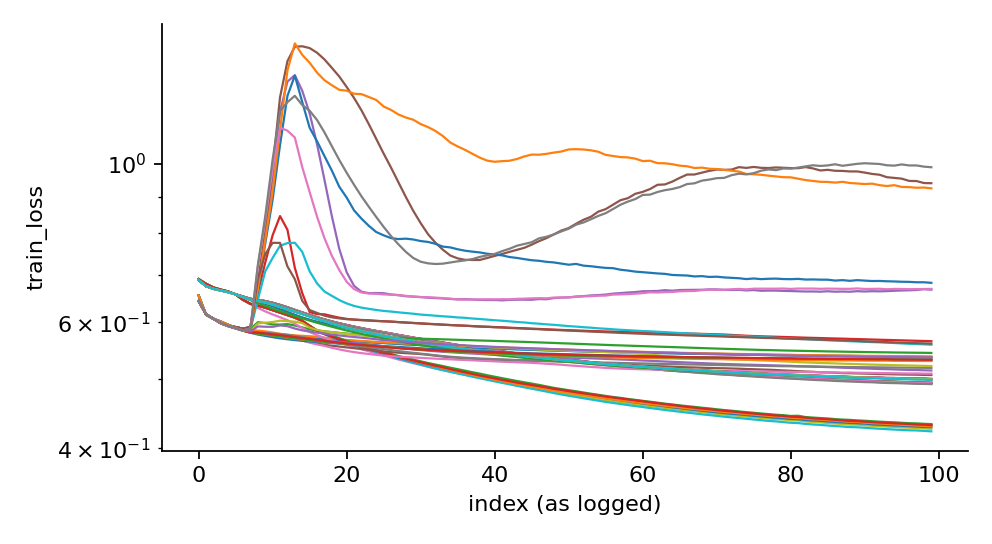
\includegraphics[width=\textwidth]{curve_train_loss.png}
\caption{\texttt{train\_loss}, the mean over seeds per cell.}
\label{fig:curve-1}
\end{figure}
\begin{figure}[tbp]
\centering
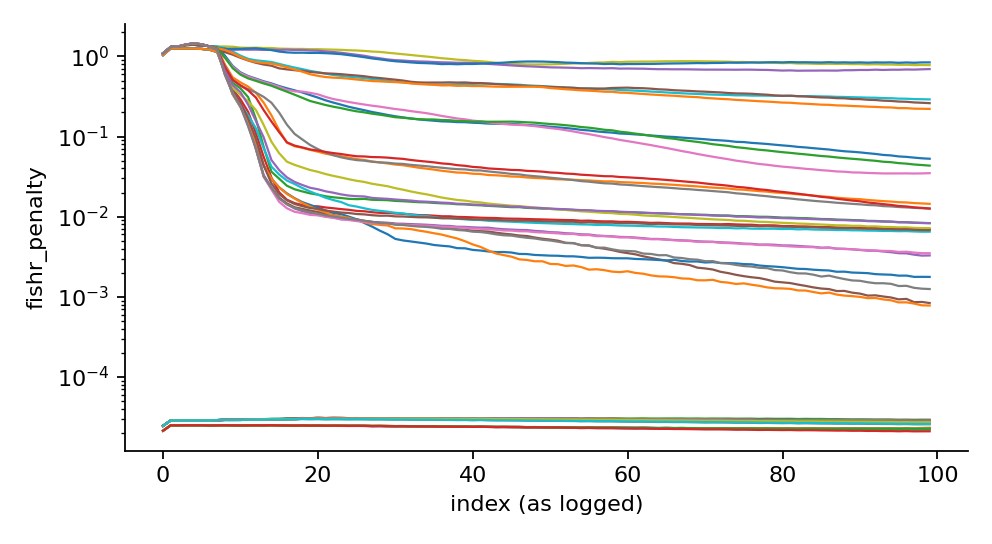
\includegraphics[width=\textwidth]{curve_fishr_penalty.png}
\caption{\texttt{fishr\_penalty}, the mean over seeds per cell.}
\label{fig:curve-2}
\end{figure}
\begin{figure}[tbp]
\centering
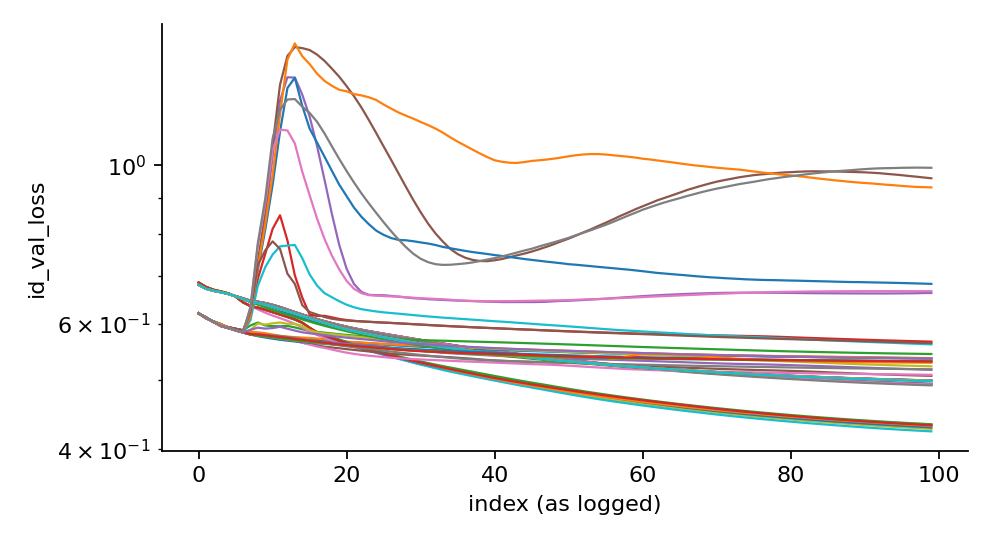
\includegraphics[width=\textwidth]{curve_id_val_loss.png}
\caption{\texttt{id\_val\_loss}, the mean over seeds per cell.}
\label{fig:curve-3}
\end{figure}

\section{Configuration}
The base configuration every run shares (frozen hash \texttt{7237e0b98779}); factor levels are in \autoref{tab:summary-ood_len_f1}.
{\footnotesize
\begin{verbatim}
task:
  name: MinCoinChangeDataset
  value_range:
  - 1
  - 10
  target_range:
  - 10
  - 20
  weight_range: null
  adversarial_range:
  - 10
  - 30
  noise_prob: 0.0
data:
  train_lengths:
  - 4
  - 5
  - 6
  - 7
  - 8
  ood_lengths:
  - 12
  - 16
  - 64
  ood_value_range:
  - 11
  - 21
  ood_noise_range:
  - 1
  - 5
  ood_noise_prob: 0.5
  n_per_length: 20000
  n_eval_per_length: 2000
  curve_eval_limit: 256
model:
  d_model: 64
  n_heads: 2
  num_layers: 1
  dropout: 0.0
  tropical_impl: legacy
optim:
  lr: 0.0001
  epochs: 100
  batch_size: 100
  eval_batch_size: 256
fishr:
  ema: 0.95
  anneal_iters: 1500
  reset_optimizer: true
\end{verbatim}
}
Store: \texttt{campaigns/tropical/MinCoinChange/results}.
\end{document}